\documentclass[fleqn,10pt]{wlscirep}
\usepackage[utf8]{inputenc}
\usepackage[T1]{fontenc}
\usepackage{bm}
\usepackage{caption}
\usepackage{subcaption}
% \captionsetup[subfigure]{justification=justified,singlelinecheck=false}
\usepackage{tikz}
\usepackage{newtxmath} % MER: Prettier math
\usepackage{cleveref} % MER: Allows \Cref (but use Section X.Y not Subsection X.Y)
\usepackage{booktabs} % MER: Prettier tables

\usepackage{graphicx}
\usepackage{subcaption}
\usepackage{tikz}
\usepackage{float}
\usepackage{amsmath}
\usepackage{siunitx}
\usetikzlibrary{quotes}
\usetikzlibrary{arrows,decorations.pathmorphing,backgrounds,positioning,fit,petri}

\graphicspath{{figures/}}

\captionsetup[subfigure]{justification=justified,singlelinecheck=false}

\title{In-silico molecular enrichment and clearance of the human intracranial space}
\author[1,x]{Marius Causemann}
\author[1,x]{Miroslav Kuchta}
\author[1,x]{Rami Masri}
\author[1,*]{Marie E. Rognes }
\affil[1]{Department of Numerical Analysis and Scientific Computing, Simula Research Laboratory, Oslo, Norway}
\affil[x]{Author order to be discussed.}
\affil[*]{meg@simula.no}

\newcommand{\rami}[1]{\textcolor{blue}{#1}}
\newcommand{\mer}[1]{\textcolor{magenta}{#1}}
\newcommand{\mar}[1]{\textcolor{violet}{#1}}
\newcommand{\discuss}[1]{\textcolor{red}{#1}}
\newcommand{\fixme}[1]{\textcolor{red}{#1}}
\newcommand{\draft}[1]{\textcolor{gray}{#1}}
%\newcommand{\brain}{\Omega_{\rm{PAR}}} 
%\newcommand{\sas}{\Omega_{\rm CSF}}
%\newcommand{\spinal}{\Gamma_{\rm SAS}}
%\newcommand{\skull}{\Gamma_{\rm{skull}}}
\newcommand{\gin}{g_{\rm{influx}}}

\newcommand{\R}{\mathbb{R}}
\newcommand{\foralls}{\forall \,}

%\affil[+]{these authors contributed equally to this work}

%\keywords{Keyword1, Keyword2, Keyword3}

\begin{abstract}
\end{abstract}
\begin{document}

\flushbottom
\maketitle
% * <john.hammersley@gmail.com> 2015-02-09T12:07:31.197Z:
%
%  Click the title above to edit the author information and abstract
%
\thispagestyle{empty}


%%%%%%%%%%%%%%%%%%%%%%%%%%%%%%%%%%%%%%%%%%%%%%%%%%%%%%%%%%%%%%%%%%%%%%%%%%%%%%%%%%%%%

\mer{MER: Target length: 5000 words, 4-6 figures: 600 words Intro. 1400 words Methods. 2000 words Results. 1000 words Discussion.}


\section*{Introduction}


Molecular transport in perivascular spaces (PVSs) is established as a key pathway for human brain clearance and delivery. Previous studies indicate that molecules move rapidly in the subarachnoid space (SAS) and in PVSs surrounding pial arteries. Here, we aim to model and study this transport in a full pial perivascular and/or vascular network embedded in the SAS.  

Motivation: as indicated by~\cite{iliff2012paravascular}, referring to
Cserr, Phys Rev., 1971, bulk convective flow may be more important for
larger species (larger distances) and larger molecules.

\section*{Background}

\mer{Point from Miro: Goriely and scaling from mice to men.}

\begin{enumerate}
\item
  Communication between perivascular spaces and the subarachnoid space
  \begin{itemize}
  \item
    Rennels et al~\cite{rennels1985evidence} infused tracer into the lateral cerebral ventricles and subarachnoid space of cats (and one dog) and observed that the tracer distributed in a perivascular pattern. The tracer distributed more rapidly around arterioles than around capillaries and veins. Importantly, the rapid paravascular influx was modulated by arterial pulsatility and in particular reduced by reduced vessel pulsatility. They directly postulate that ``fluid circulation through the central nervous system occurs via paravascular pathways'', and discuss both mixing and pumping as pulsatility-associated mechanisms for transport. 
  \item
    Weller and coauthors conducted pioneering studies of perivascular spaces, flow and transport~\cite{zhang1990interrelationships, zhang1992directional, weller2005microscopic}. They identified thin sheaths of pial cells surrounding arteries and arterioles (but not veins or venules) on the brain surface and within the human brain itself~\cite{zhang1990interrelationships}. Further, they observed that tracers spread along perivascular (arterial, venous and capillar) spaces in (rat) grey matter, and in the subarachnoid space (to the cribriform plate and nasal lymphatics).   
  \item
    Ichimura et al~\cite{ichimura1991distribution} study the distribution of large molecular weight tracers in the subarachnoid and surface perivascular spaces and within the cortex in rats. They observed rapid spread in perivascular spaces, and that tracers injected into the CSF of the subarachnoid space spread also into subarachnoid and cortical perivascular spaces. In conclusion, they highlight the presence of an extensive perivascular network, and report of some bulk flow, but slow and of variable directionality - in contrast to e.g Rennels et al~\cite{rennels1985evidence}. 
  \item In a series of papers, Bakker and coauthors study perivascular anatomy and solute transport~\cite{bedussi2017paravascular, bedussi2018paravascular}. They find that the subarachnoid space, the cisterns, ventricles and penetrating periarteriolar spaces form a continuous cerebrospinal fluid-filled space surrounding and penetrating into the murine brain \cite{bedussi2017paravascular}. Moreover, they demonstrate pulsatile and directional (antegrade) flow in perivascular (predominantly periarterial) spaces on the brain surface \cite{bedussi2018paravascular}. 
  \item
    Iliff et al~\cite{iliff2012paravascular} observed rapid movement of tracer (injected in the cisterna magna) along the outside of surface arteries and penetrating arterioles in mice, and state this is in agreement with the presence of perivascular sheaths as reviewed by Weller~\cite{weller2005microscopic}.
  \item
    The architecture of perivascular spaces in and around the rat brain was also studied in detail by Thorne and colleagues~\cite{pizzo2018intrathecal, hannocks2018molecular}. Hannocks et al~\cite{hannocks2018molecular} characterize the molecular composition of different perivascular compartments. Pizzo et al~\cite{pizzo2018intrathecal} emphasizes the presence of stomata or pores present on the interface between blood vessels and the CSF in the subarachnoid space. Neither seem to quantitatively report on PVS widths.
  \item Mestre et al~\cite{mestre2022periarteriolar} study the properties of pial perivascular spaces in detail in mice, and in particular the structure and coverage of pial cells and pial layers surrounding leptomeningeal arteries (and arterioles). They report of pial cells forming sheaths for larger ($> 10000 \mu$m$^2$ cross-section lumen area) surface arteries and partially coverage for smaller surface arteries, with higher coverage in ventral SAS regions. They find that these pial layers do not form an impermeable barrier to small molecules. Importantly, they also study the pial coverage in aged and Alzheimer's model mice, and find significant and complex changes in these pial structures.
  \item
    In humans, Eide and Ringstad investigate cerebrospinal fluid tracer transport in the human subarachnoid space after intrathecal injection~\cite{eide2024functional}. They observe tracer enrichment antegrade along the major cerebral arteries, and enrichment of the nearly cerebral cortex. They also consider variations in different patient cohorts and find impaired transport in iNPH patients with increased perivascular space size. They report of tracer enrichment in donut-shaped perivascular spaces. The timings here may be the best estimate of human PVS flow speeds. 
  \item
    Yamamoto et al~\cite{yamamoto2024perivascular} also report of contrast-enhancement in human PVS.
  \end{itemize}
\item
  Shapes and sizes of the perivascular spaces\footnote{The area $A$ of
  a circle with inner radius $R_1$ is $A = \pi R_1^2$. The area $A_2$
  of an annulus with inner radius $R_1$ and outer radius $R_2$ is $A_2
  = \pi (R_2^2 - R_1^2)$. The width of this annulus is $R_2 -
  R_1$. The ratio PVS/lumen area can thus be estimated as $A_2/A =
  (R_2^2 - R_1^2)/R_1^2$. For example, if $R_2 = n R_1$ ($n = 2
  \rightarrow$ PVS width equal to lumen radius, $n = 3 \rightarrow$
  PVS width equal to lumen diameter), then $A_2/A = n^2 - 1$. However,
  if the annulus has an elliptic outer boundary with radii $R_a$ and
  $R_b$, then its area is $A_e = \pi (R_a R_b - R_1^2)$, and so in the
  extreme case where $R_a > R_b = R_1$, the area is $\pi R_1 (R_a -
  R_1)$, and the PVS/lumen area ratio is $A_e/A = (R_a -
  R_1)/R_1$. And so, for $R_a = n R_1$, then $A_e/A = n-1$.}. Note
  that representing the surface PVS as annular cylinders is a
  simplification, and several studies emphasize the asymmetric nature
  of the PVS shape~\cite{mestre2018flow, tithof2019hydraulic,
    vinje2021brain, raicevic2023sizes}. Moreover, do not forget that
  the sizes of mice and humans are orders of magnitude apart.
  \begin{itemize}
  \item
    Ichimura et al~\cite{ichimura1991distribution} report on a typical
    perivascular width of $1-10\mu$m, but broader around vessel
    bifurcations in the rat subarachnoid space (fixed specimens).
  \item Foley et al~\cite{foley2012realtime} report on perivascular
    space width within rat cortex of $8-10\mu$m for arterioles of
    $\approx$30$\mu$m in diameter.
  \item
    Schain et al~\cite{schain2017cortical} report on the sizes of pial
    arteries ($6.0-11 \mu$m in diameter\footnote{Schain et
    al~\cite{schain2017cortical} state diameter rather, but the
    diameter does not match with the given area, so perhaps this
    should be the radius}) and veins ($9.4-21\mu$m) in mice, with an
    average PVS/lumen area ratio of $1.26$ for arteries and $0.13$ for
    veins. 
  \item Mestre et al~\cite{mestre2018flow} measure and characterize
    pial perivascular transport and estimate flow magnitudes in
    mice. They report a PVS/lumen area ratio of $1.4 \pm 0.1$ and a
    PVS width of $\approx 40 \mu$m which described as comparable to
    the adjacent artery (diameter). 
\item
  Raicevic et al~\cite{raicevic2023sizes} study the sizes and shapes
  of perivascular spaces surrounding pial arteries in mice in detail,
  in particular the relationship between periarterial space and lumen
  (cross-section) area and its variation with vessel area and
  location. They remark that the variation in PVS area is larger
  between PVS segments than along a single PVS segment. The PVS area
  seems to increase with the vessel area, but an affine approximation
  gives a poor fit, and from inspecting the distribution, the
  relationship seems superlinear. The peak distribution value of
  segmented PVS/lumen area is $1.12$.
  \item
    In terms of size, Bedussi et al.~\cite{bedussi2018paravascular} report a PVS width of $\approx$20$\mu$m surrounding surface arteries branching from the MCA (of diameters $45 \pm 7$ $\mu$m). Note that they include both data from mice and OCT data from humans. They report of human PVS size linearly related with the vessel size (and in the range 0.1--0.35 mm for vessels of diameter 0.1--0.5 mm).
  \item Vinje et al~\cite{vinje2021brain} and references therein illustrates the location and characteristics of human pial perivascular spaces, using human OCT data from the Bakker lab.
  \item Bollman et al~\cite{bollmann2022imaging} image the human pial vasculature at high resolution (7T), and report of pial arterial diameters in the range $50-280 \mu$m.
\item
  Smets et al~\cite{smets2024perivascular} study the size of
  perivascular spaces surrounding pial arteries and veins in mice
  (in-vivo), with particular emphasis on the properties of perivenous
  spaces. They observe the PVS as two ``triangular spaces'' adjacent
  to both arteries and veins, and separated from the subarachnoid
  space by a membrane (see also references
  to~\cite{zhang1990interrelationships, pizzo2018intrathecal,
    mollgard2023mesothelium}). They found that the cross-section area
  of the PVS correlates with the lumen area both for pial arteries
  and veins, but not for penetrating vessels. They report a
  PVS-to-lumen-area ratio of 0.43 for arteries and 0.35 for veins.
\item
  Personal communication (Ringstad, Oct 15 2024)~\cite{eide2024functional}: a typical blood vessel in the M2-segment of the MCA is 1.56 mm in diameter ($2 R_1$) with an annular PVS of width ($R_2 - R_1$) 1.23 mm and total PVS diameter $2 R_2$ of 3.93. In iNPH patients, extreme outliers are observed; e.g. still with annular PVS, but not concentric (shifted vessel), for vessel diameter of 2 mm and PVS width from 1.1 mm to 6.0 mm.
  \end{itemize}
\item
  Perivascular hydraulic resistances. The hydraulic resistance of
  perivascular spaces has been studied extensively, with key
  contributions from Thomas, Kelley, Tithof and collaborators~\cite{tithof2019hydraulic}.
  \begin{itemize}
  \item Boster et al.~\cite{boster2024hydraulic} study methods of estimating the hydraulic resistance of perivascular spaces via in-vivo imaging-based 3D reconstructions of pial perivascular spaces in mice; they report of hydraulic resistances of the order $1.7 \times 10^6 - 8.9 \times 10^5$ mmHg·min/mL/m).
  \end{itemize}
\item
  Perivascular flow characteristics: magnitudes and directionality?
  \begin{itemize}
  \item
    Rennels et al~\cite{rennels1985evidence} highlight in their
    Discussion that
    \begin{quote}
      This evidence of fluid displacement in both directions through
      the perivascular spaces suggest either that influx and efflux
      occur intermittently through the same perivascular spaces or
      that these fluid movements occur via separate populations of
      perivascular spaces.
    \end{quote}
  \item
    Ichimura et al~\cite{ichimura1991distribution} found that albumin in the subarachnoid periarterial space moved 1.5 mm away from the injection site in about 7 minutes, thus a net speed of around $3.6 \mu$m/s. 
  \item
    Hadaczek et al~\cite{hadaczek2006perivascular} studied the role of arterial pulsations in more detail, following up on~\cite{rennels1985evidence}.
  \item Foley et al~\cite{foley2012realtime} study perivascular transport characteristics of nanoparticles injected in the cerebral cortex of rats, though in the context of convection-enhanced delivery.
  \item
    In terms of movement, Bedussi et al~\cite{bedussi2018paravascular} found a net movement of particles in surface PVS (in mice) in the antegrade (same direction as blood flow) direction with an average velocity of $17 \pm 2\mu$m/s, and a mean amplitude of the pulsatile motion of $14 \pm 2 \mu$m.
\item Mestre et al~\cite{mestre2018flow} report a mean (averaged over time and space) flow speed of $18.7 \mu$m/s (root-mean-square velocity?) with net transport in the antegrade direction (near the MCA, in mice).
\item
  Asgari et al~\cite{asgari2016glymphatic} model tracer transport in axial periarterial spaces, highlight the negligible net (directional, bulk) flow induced by arterial wall pulsations at physiologically realistic wavelengths, but also the contributions from wall pulsations to dispersion. 
\item
  Rey and Sartinoranont~\cite{rey2018pulsatile} examine pulsatility as a driver for net flow in perivascular spaces within the brain parenchyma via a hydraulic network models, again highlighting the negligible net flow induced by vascular wall movements, but significant pulsatile flow and thus potential for dispersive effects~\cite{watson1983diffusion, asgari2016glymphatic}.
\item
  Rey et al~\cite{rey2023perivascular} consider a comprehensive ex-vivo perivascular network segmentation in the rat brain following in-vivo intraventricular contrast infusion. They highlight the numerous connections between the ventricular system and the perivascular spaces, including long perivascular segments extending from the surface and deep into the brain. 
\item
  In the context of dispersion, see also~\cite{asgari2016glymphatic, keith2019dispersion, troyetsky2021dispersion}
\item
  Wright et al~\cite{wright2024coupled} study the dynamics (waveforms over time) of human arterial blood flow (with resting-state fMRI) and perivascular CSF flow (with dynDWI, apparent diffusion coefficient (mm$^2$/s)). The waveforms seem coupled, with the arterial peak preceding the CSF peak by around 0.06 (of a cardiac cycle). The report ADC in the PVS on the order $2.5-5.5 \times 10^{-3}$ mm$^2$/s, with alterations in the coupling with age.
\item
  Boster and coauthors~\cite{boster2023artificial, toscano2024infeering} estimate perivascular flow parameters in mice via physics-informed neural networks (e.g.~pressure gradients, hydraulic resistances, shear stresses). Boster et al~\cite{boster2023artificial} estimate PVS pressure gradients on the order of $0.7-5 \times 10^{-4} \unit{Pa/\mu m}$\footnote{Note that 
  \begin{equation}
    1 \times 10^{-4} \, \unit{Pa/\mu m} = 1 \times 10^{2} \, \unit{Pa/m} \approx 100/133 \unit{mmHg/m} \approx 0.75 \unit{mmHg/m}
  \end{equation}
   }, downstream velocity component of $12.75 \pm 6.25 \unit{\mu m/s}$. 
  \end{itemize}
\item
  Broggini et al~\cite{broggini2024long} describe long-wavelength traveling waves of vasomotion (0.1 Hz) in pial arterioles in mice. They find waves traveling in both directions, with waves exiting the surface of the cortex more often than chance (85 of 140 exit). ``The wavelength of the observed pial waves is long, typically 20 mm or twice the length of the mouse cortex (inset in Figure 4C).'', with relative amplitudes in the range 0.02--0.12 in pial arterioles.
\item
  Kedarasetti et al~\cite{kedarasetti2020functional} model functional hyperemia waves (aka stimulus-induced vasomotion, see also van Veluw et al~\cite{vanveluw2020vasomotion}). Note that the directionality of vasomotion is classically thought to be in the opposite direction of the blood flow.
\item
  Note that Gokina et al~\cite{gokina1996electrical} report of spontaneous rhythmic contraction in human pial arteries.
\end{enumerate}
Cerebrospinal fluid flow
\begin{itemize}
\item
  Sweetman and Linninger~\cite{sweetman2011cerebrospinal} model the flow of cerebrospinal fluid in the cranial and spinal subarachnoid space of a healthy human driven by pulsatile displacement of the upper walls of the lateral ventricles representing volumetric changes of the vasculature, with model predictions in good agreement with clinical observations of CSF velocity magnitude and stroke volume. 
\item Causemann et al.~\cite{causemann2022human}
\item
  Vinje et al.~\cite{vinje2019respiratory} consider clinical measurements of intracranial pressure differences and human CSF-space geometries together with computational modelling to study CSF flow patterns in the aqueduct. They estimate the pressure gradient across the cerebral aqueduct resulting from a CSF production of 0.5L/day to be $0.009 \pm 0.006$ mmHg/m.
\item Hornkjøl et al~\cite{hornkjol2022csf} model CSF flow and solute transport in the human SAS and brain parenchyma. 
\end{itemize}

%%%%%%%%%%%%%%%%%%%%%%%%%%%%%%%%%%%%%%%%%%%%%%%%%%%%%%%%%%%%%%%%%%%%%%%%%%%%%%%%%%%%%
\section*{Results}

~ 2000 words and 7 subsections - around 300 words each?
\begin{enumerate}
\item
  ``A digital twin'' for molecular enrichment and clearance in human intracranial spaces
\item
  CSF flow, the role of production versus no/cardiac/respiratory
  dispersive effects on tracer trajectories, flow bifurcation. With and without tentorium cerebellum.
\item
  ``The role'' of PVS flow speed
\item
  ``The role'' of PVS sheaths and permeability
\item
  ``The role'' of PVS size versus pathologies $R_2 = 3 R_1$ instead of $R_2 = 2 R_1$?
\item
  Clearance from the CSF spaces - with and without low pressure veins, but keeping the intrathecal source of solute. Quantities of interest?
\item
  Clearance from the parenchyma - with and without low pressure veins, $c_0 = 1.0$.
\end{enumerate}

\begin{figure}
     \begin{subfigure}[b]{0.45\textwidth}
         \centering
         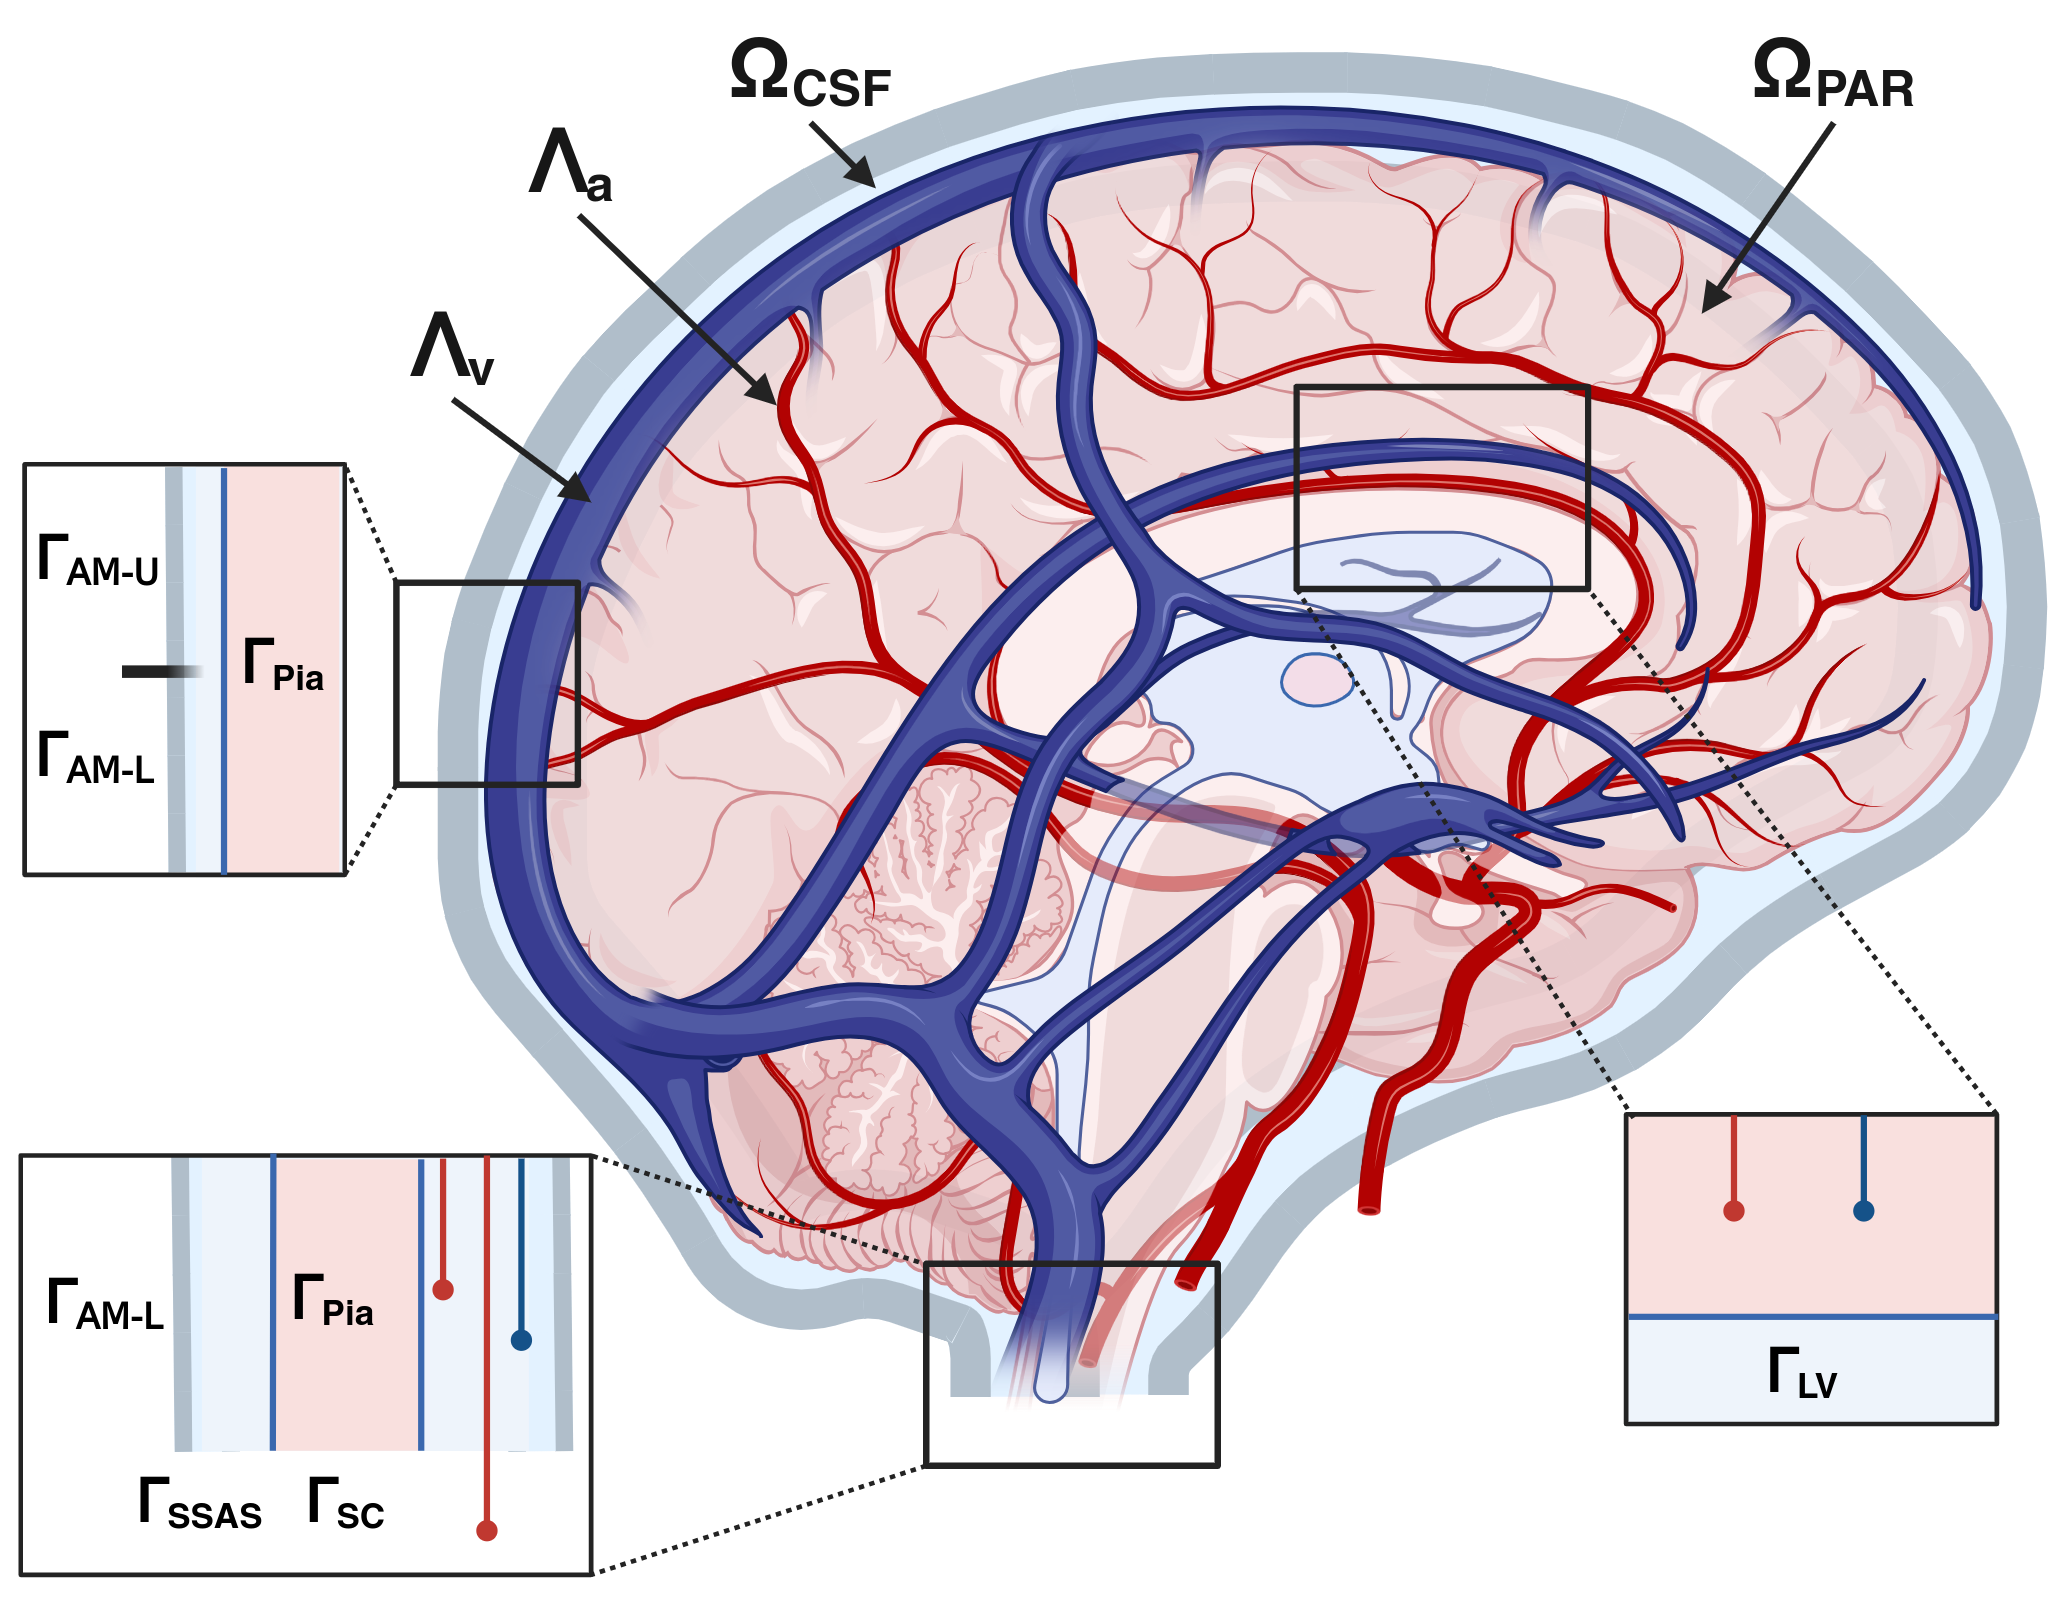
\includegraphics[width=\textwidth]{figures/Brain-PVS-callouts.png}
     \end{subfigure}
     \hfill
     \caption{a) Illustration of the different intracranial domains
       considered with labels;}
     \label{fig:intracranial_domains}
\end{figure}


\subsection*{High-fidelity in-silico predictions of intracranial solute transport and exchange}

\begin{itemize}
\item
  Present mathematical and computational model and geometries (\Cref{tab:scenarios}). 
\item
  Highlight computational model availability, open source code.
\item
  Provides an interactive in-silico platform for studying intracranial solute transport -- distribute such that anyone can run (possibly try to recruit MinRK if advantageous).
\end{itemize}

\draft{\lipsum[1]}


\subsection*{II: CSF flow}


Flow of CSF through the SAS and the ventricular system is a crucial driver of transport in the human brain environment.
While cardiac- and respiratory induced oscillatory flow increases mixing, the production of CSF in the choroid plexus creates a steady advective flow within the CSF-filled spaces of the cranium \cite{hornkjol2022csf}. 
We construct a 3D model of the SAS and the ventricular system (\Cref{fig:csf}A,B and C) and compute CSF flow fields for three different scenarios: CSF production in the choroid plexus, CSF flow at systolic peak blood inflow and CSF flow in response to free breathing.

% production flow simulation
To simulate the production-driven flow, we impose an inflow of $400\,$ml/day \cite{nilsson1992circadian} across the surface of the lateral ventricle and allow a resistive outflow across the upper convexity of the arachnoid mater, leading to a total pressure drop of $26\,$mPa between the production and outflow sites. A maximum flow velocity of $1.8\,$mm/s is attained in the aqueduct, while the mean velocity in the SAS is $2.6\,\mu$m/s (\Cref{fig:csf} E).

%The Stokes system is solved with the finite element software $FEniCS$, stored and then subsequently read for all the relevant solute transport simulations. See Figure~\ref{fig:csf} for a streamline visualization of the obtained velocity profile and \Cref{sec:details_numerical_method} for details on the numerical algorithm employed.

% cardiac pulsatility
Assessing the effect of cardiac-driven dispersion, we compute a steady CSF flow field at peak cranial blood volume during the cardiac cycle. We mimic resulting the reduced CSF space volume by imposing an inflow of $8\,$ml/s \cite{baledent2014imaging} and $0.31\,$ml/s \cite{vinje2019respiratory} across the arachnoid mater and the lateral ventricle surface, respectively. We allow free outflow into the spinal SAS. In addition, we upscale the obtained pressure field to account for the lack of pulsatile inertial effects in our model (see \ref{sec:dispersion_details}). In this scenario, we observe a pressure drop of $8.5\,$Pa between lateral ventricles and the spinal SAS and a maximum flow velocity of $16.7\,$cm/s in the aqueduct (\Cref{fig:csf}F and J).
Next, we estimate a spatially varying dispersion enhancement factor $R$ from cardiac-induced pulsatility by combining the computed pressure field with the theory of shear-augmented dispersion (see \Cref{sec:dispersion_details}). We find that cardiac-induced pulsatile CSF flow increases the effective diffusion by up to two orders of magnitude in the aqueduct and around the cisterna magna, but has little effect in most of the SAS ($R < 1$) (\Cref{fig:csf} G and K). 

% respiratory pulsatility
Employing the same methodology, we estimate the respiratory contribution to dispersive mixing by computing the CSF flow field driven by an inflow of $0.121\,$ml/s \cite{liu2024using} and $0.879\,$ml/s across the lateral ventricular wall and the arachnoid mater, respectively. This amounts to a respiratory peak flow volume of $1\,$ ml/s at the craniocervical junction \cite{gutierrez2022effect}. While the resulting flow velocities are about one order of magnitude lower than their cardiac-induced counterparts (see \Cref{fig:csf}H and L), respiratory dispersive mixing reaches a factor of up to 350 due the lower respiratory frequency ($0.25\,$Hz) (\Cref{fig:csf}I and M).


% tracer trajectory of the standard model
Next, we predict the advective and dispersive spreading of $0.5\,$mmol intrathecally injected Gadobutrol in CSF-filled spaces, the parenchymal tissue and PVSs around arteries and veines. One hour post-injection, 
\begin{itemize}
    \item 
\end{itemize}


% tracer trajectory of model variations
model variations are hard to fit on a one page figure -

\begin{itemize}
    \item only dispersion model: No production flow. Tracer remains in the subtentorial regions, in cerebellum, brain stem and surrounding CSF. In contrast to other models, it travels up the ventricular system - similar to what is observed in iNPH patients?
    \item Low dispersion model: account for uncertainty (or pathologies with impaired pulsatile motion?) - tracer exclusively spreads in the frontal half of the brain. Bifurcation of CSF production flow field: flow bifurcates around the midbrain in two directions: a) through the quadrigeminal cistern into the longitudinal fissure and b) frontally around the brain through the outer SAS. Only models with "enough" dispersion enable tracer to follow trajectory a).
    \item without tentorium: 
\end{itemize}

\begin{figure}[h!]
\centering 
\includegraphics[width = 0.9 \linewidth]{paper/figure2-tight.png}
\caption{\mer{A) Illustration of 3D-domains; (B) Illustration of
    relevant boundaries; C) CSF flow induced by CSF production; D) CSF
    flow induced by peak arterial influx/peak volumetric influx of
    cardiac cycle; E) Computed dispersion factor.}}
\label{fig:csf}
\end{figure}  

\subsection*{III: Perivascular flow}

\draft{\lipsum[1]}

\begin{figure}
    \centering
    \begin{subfigure}[b]{0.65\textwidth}
    \centering
    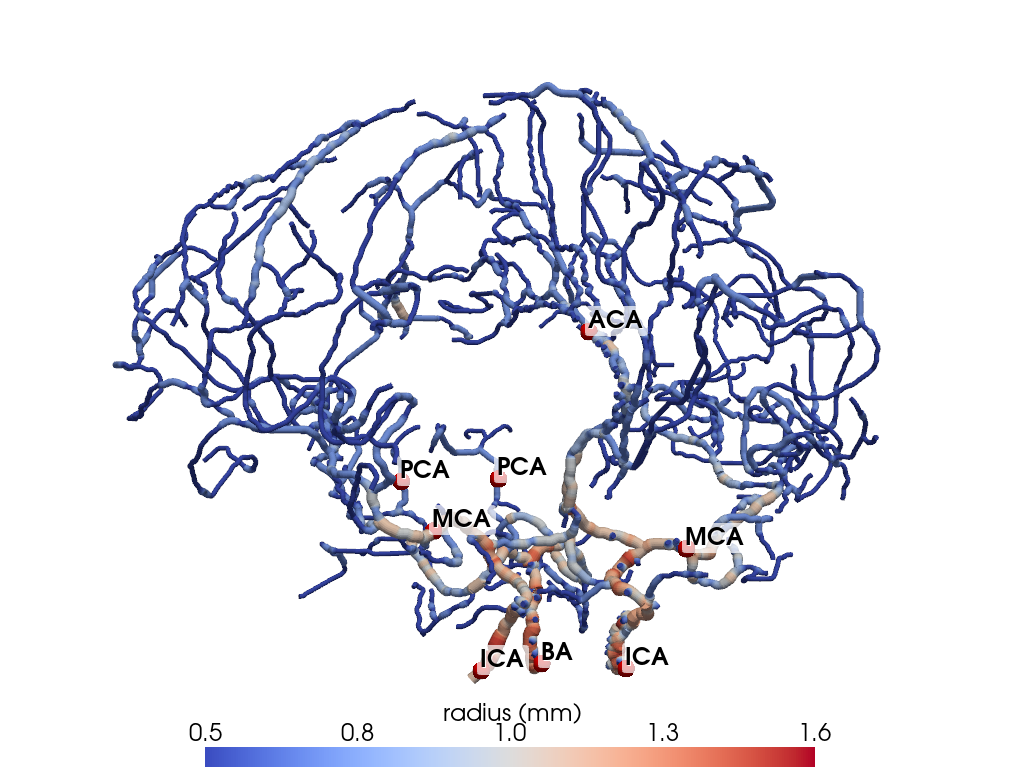
\includegraphics[width = \linewidth]{figures/labeled_arteries.png}
    \end{subfigure}
     \begin{subfigure}[b]{0.3\textwidth}
    \centering
    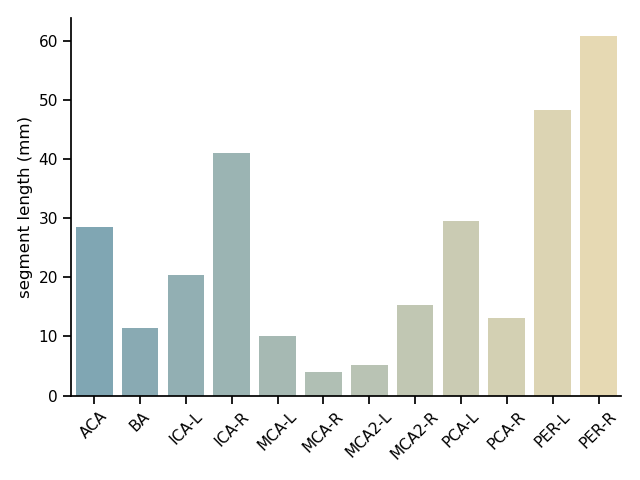
\includegraphics[width =  \linewidth]{figures/vasomotion_arteries_labels_length.png}
    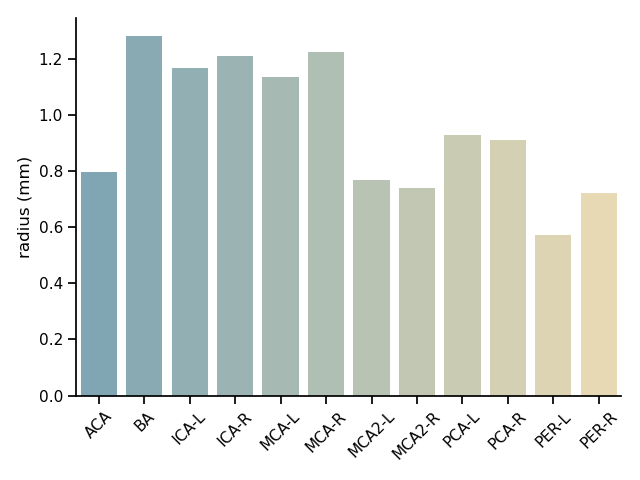
\includegraphics[width =  \linewidth]{figures/vasomotion_arteries_labels_radius.png}
    \end{subfigure}
     \begin{subfigure}[b]{0.33\textwidth}
    \centering
    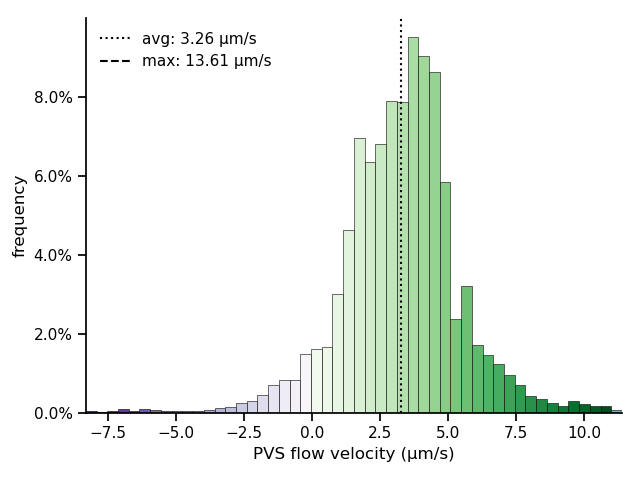
\includegraphics[width =  \linewidth]{figures/vasomotion_velocity_histo_cell.png}
    \caption{Vasomotion}
    \end{subfigure}
    \begin{subfigure}[b]{0.33\textwidth}
    \centering
    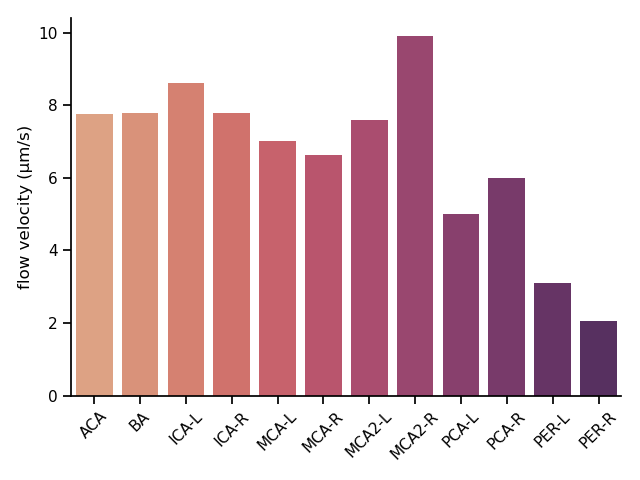
\includegraphics[width =  \linewidth]{figures/vasomotion_arteries_labels_velocity.png}
    \end{subfigure}
    \begin{subfigure}[b]{0.33\textwidth}
    \centering
    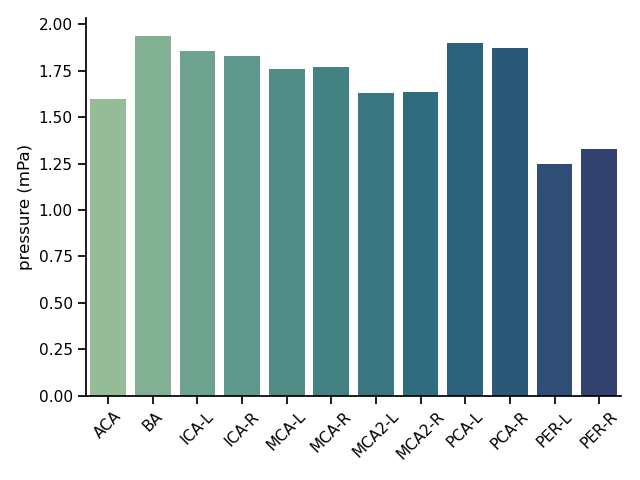
\includegraphics[width =  \linewidth]{figures/sas_flow_arteries_labels_pressure.png}
    \end{subfigure}
         \begin{subfigure}[b]{0.33\textwidth}
    \centering
    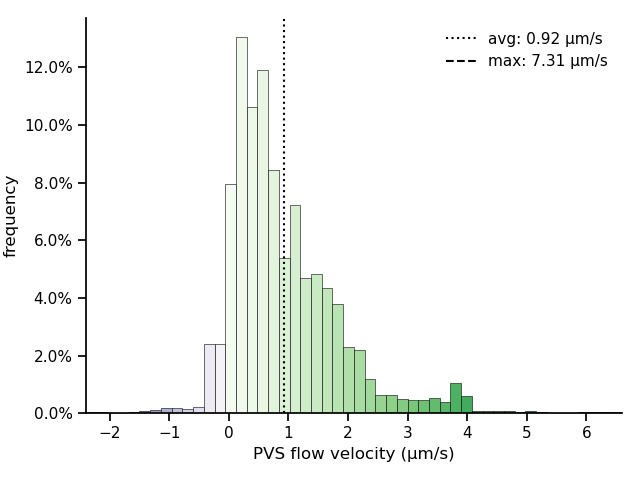
\includegraphics[width =  \linewidth]{figures/cardiac_pvs_oscillation_velocity_histo_cell.png}
    \caption{Cardiac peristaltic flow}
    \end{subfigure}
    \begin{subfigure}[b]{0.33\textwidth}
    \centering
    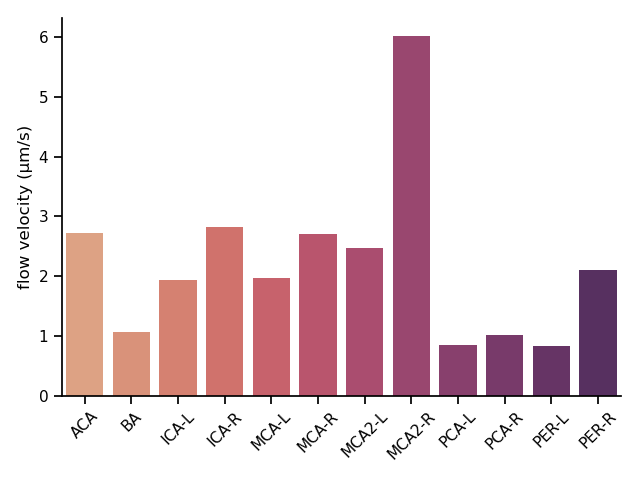
\includegraphics[width =  \linewidth]{figures/cardiac_pvs_oscillation_arteries_labels_velocity.png}
    \end{subfigure}
    \begin{subfigure}[b]{0.33\textwidth}
    \centering
    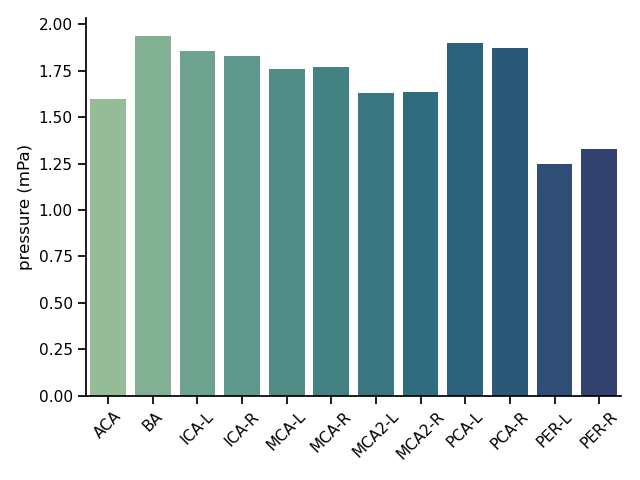
\includegraphics[width =  \linewidth]{figures/sas_flow_arteries_labels_pressure.png}
    \end{subfigure}
         \begin{subfigure}[b]{0.33\textwidth}
    \centering
    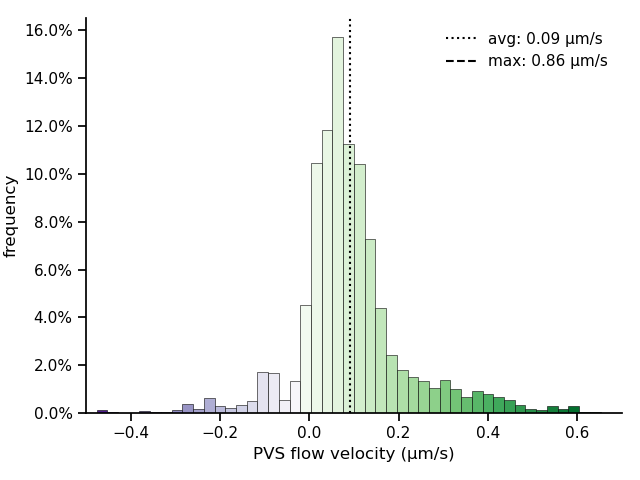
\includegraphics[width =  \linewidth]{figures/sas_flow_velocity_histo_cell.png}
    \caption{Production induced flow}
    \end{subfigure}
    \begin{subfigure}[b]{0.33\textwidth}
    \centering
    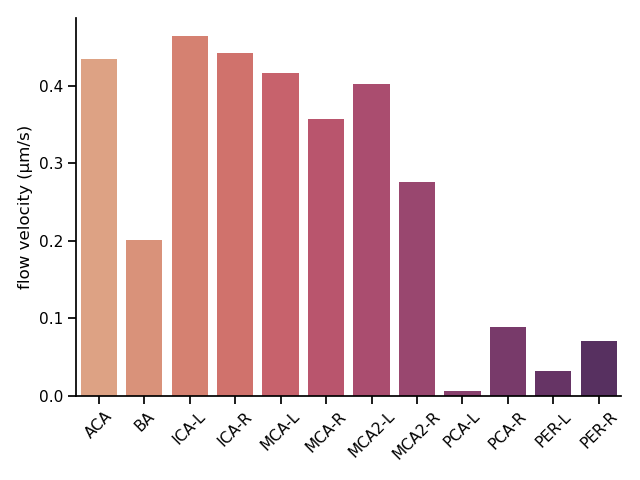
\includegraphics[width =  \linewidth]{figures/sas_flow_arteries_labels_velocity.png}
    \end{subfigure}
    \begin{subfigure}[b]{0.33\textwidth}
    \centering
    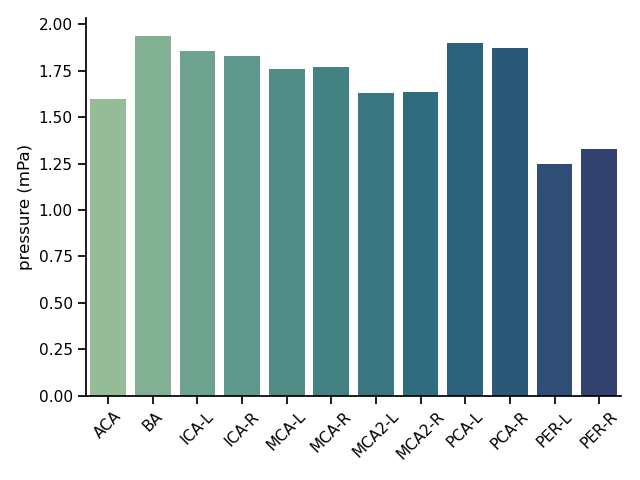
\includegraphics[width =  \linewidth]{figures/sas_flow_arteries_labels_pressure.png}
    \end{subfigure}
    %\label{fig:enter-label}
    \caption{\mer{MER: Put vasculature network illustration here. Many aspects actually. Marking of segments. Location relative to 3D. Radius etc. Marius will evaluate and suggest. Results: Group segments by logical order. For key arterial segments: average radius and length (can be moved to Supplementary if need be); pressure values; flow velocities; and then histograph with flow velocities for each mesh cell. Make sure to minorly note that ACA refers to a segment of the ACA and not the whole thing e.g.}}
    \label{fig:pvs}
\end{figure}

\Cref{fig:pvs}.

\subsection*{Structural versus functional compartmentalization of perivascular spaces}

\begin{itemize}
\item
  Are perivascular spaces functionally or structurally
  compartmentalized? Human and rodent observations indicate that
  tracers concentrate in perivascular spaces surrounding the pial and
  subarachnoid vasculature. Must these spaces be structural
  i.e.~defined by semi-permeable structural
  membrane~\cite{zhang1990interrelationships, zhang1992directional,
    mestre2018flow, eide2024functional}, or can such
  compartmentalization be a result of regions of enhanced flow or
  mixing~\cite{bedussi2017paravascular, vinje2021brain}? See also
  references in Background.
\item
  Compare Model A variations \Cref{tab:scenarios}).
\end{itemize}
\begin{figure}
\begin{subfigure}{0.5 \linewidth}
    \centering
    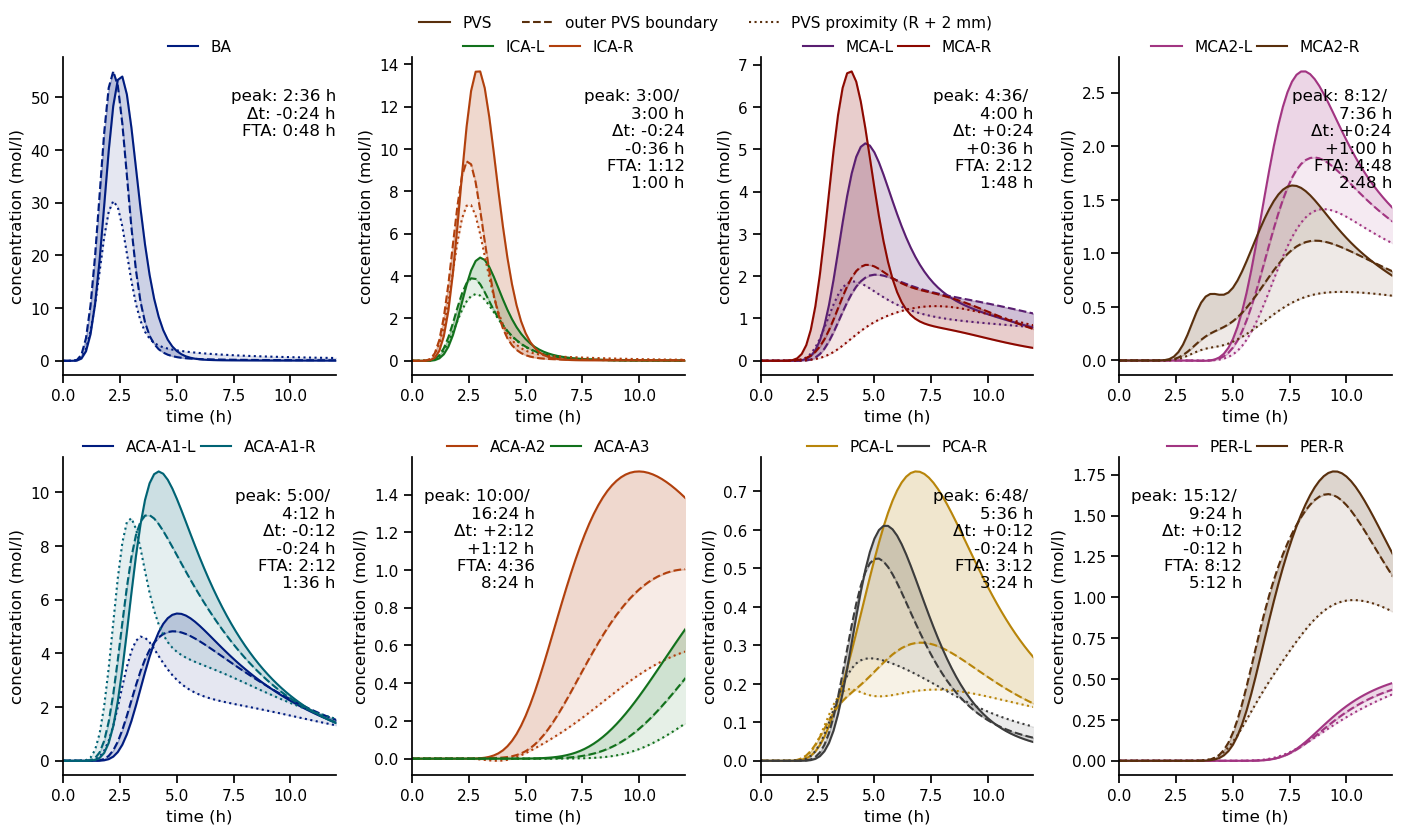
\includegraphics[width=1\linewidth]{figures/modelA_conc_at_label.png}
    \caption{B1 - $\xi$}
    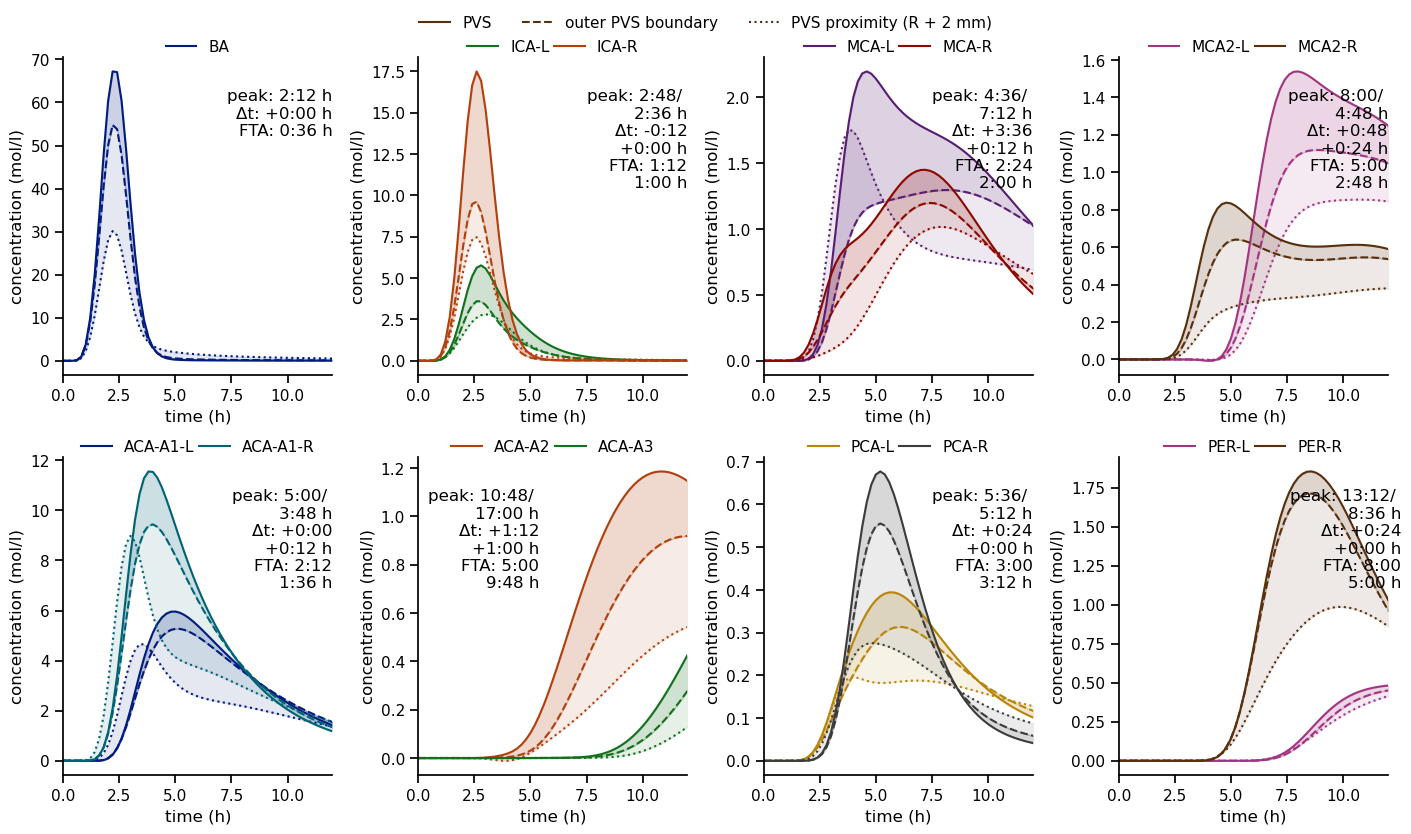
\includegraphics[width=1\linewidth]{figures/modelB1-10_conc_at_label.png}
    \caption{B1 - $10 \xi$}
    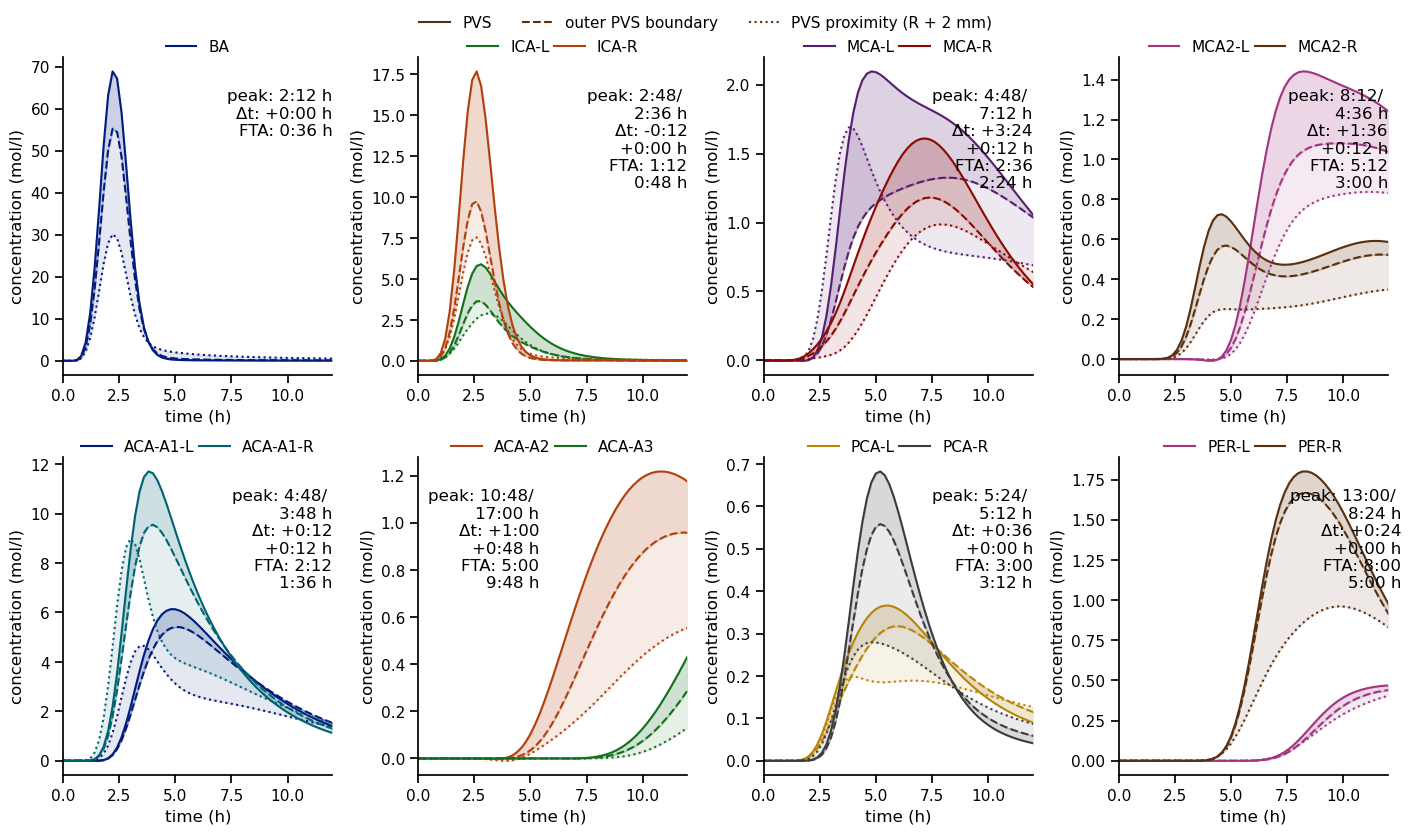
\includegraphics[width=1\linewidth]{figures/modelB1-100_conc_at_label.png}
    \caption{B1 - $100 \xi$}
    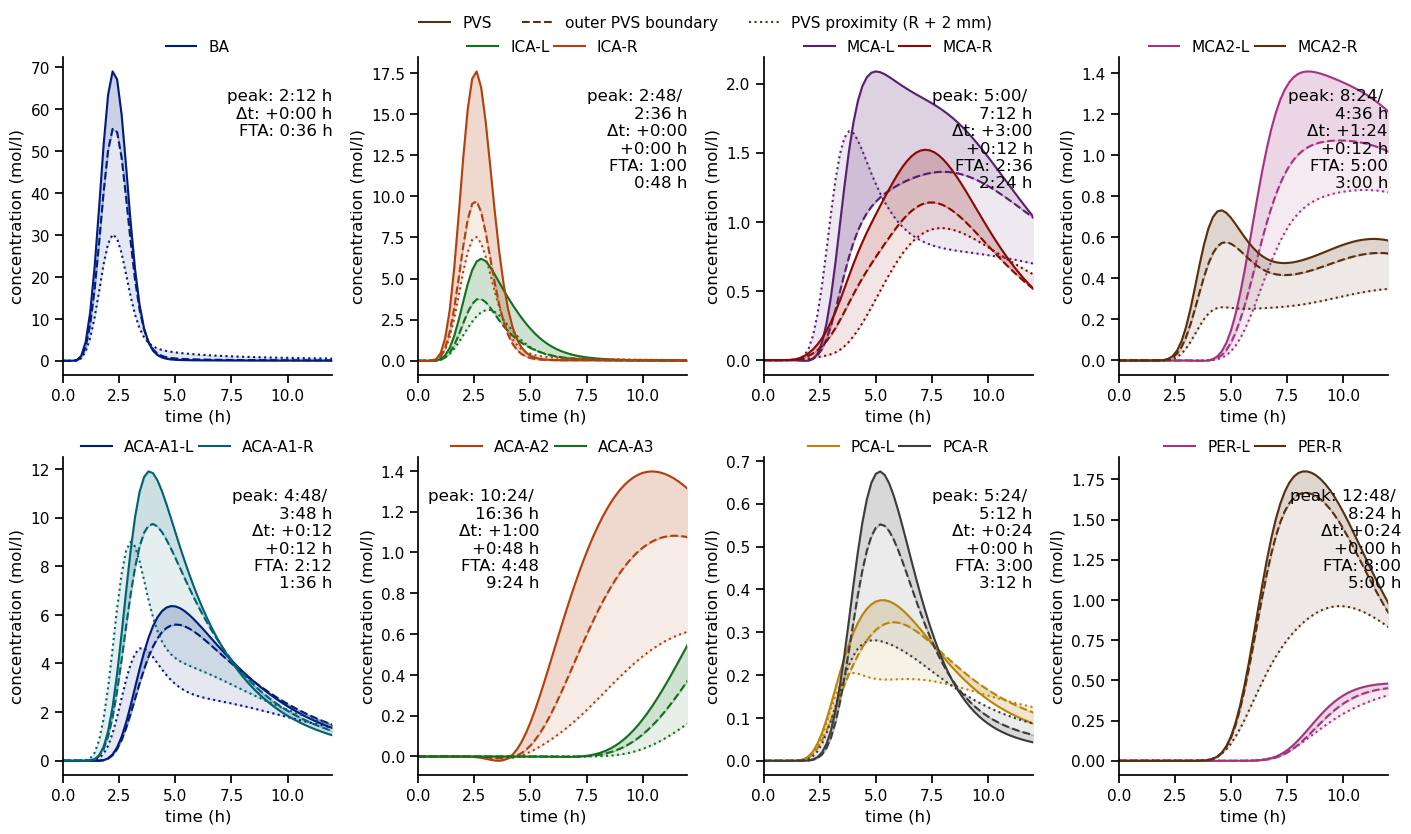
\includegraphics[width=1\linewidth]{figures/modelB1-1000_conc_at_label.png}
    \caption{B1 - $1000 \xi$}
\end{subfigure}
\begin{subfigure}{0.5 \linewidth}
    \centering
    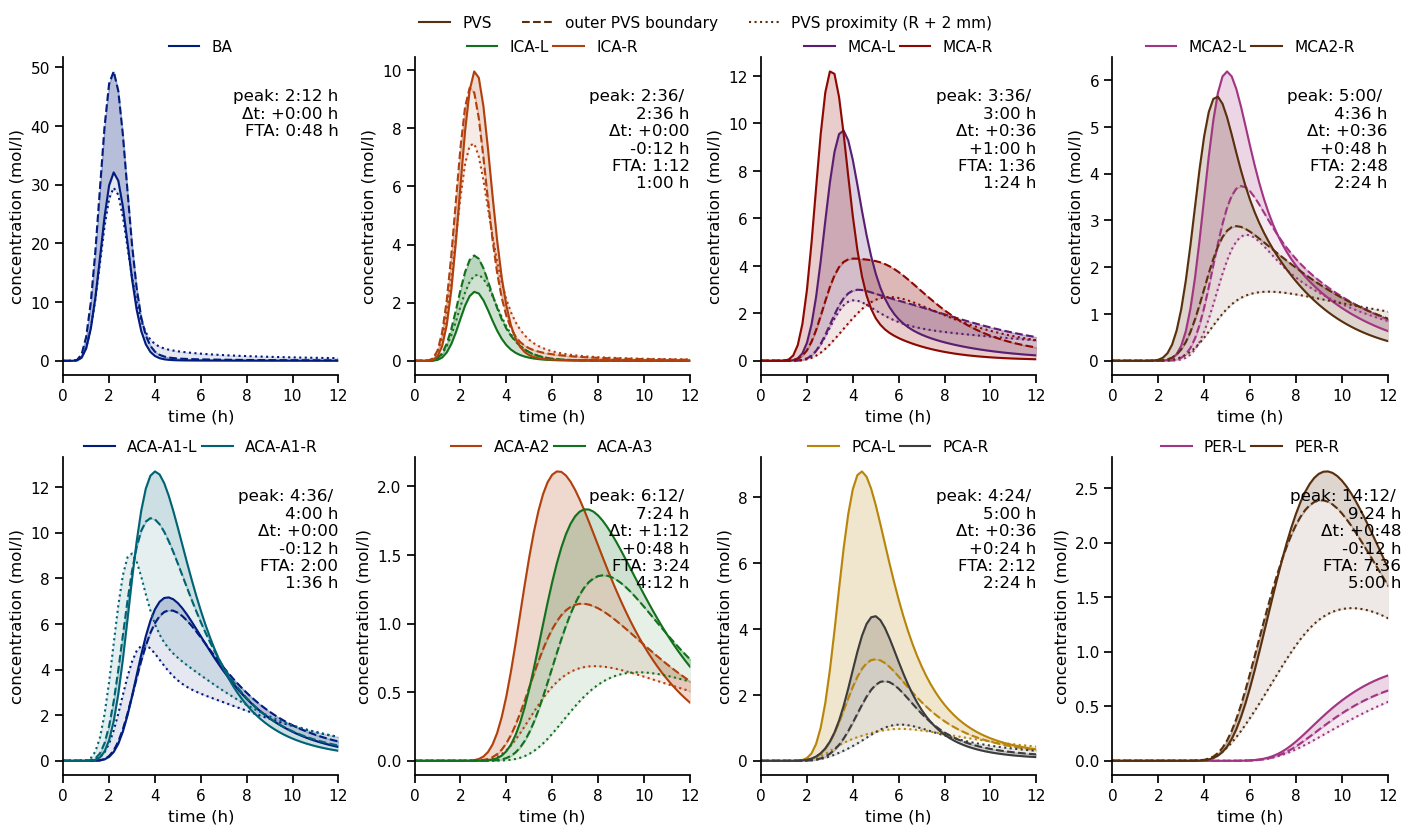
\includegraphics[width=1\linewidth]{figures/modelB2-1_conc_at_label.png}
    \caption{B2 - $\xi$}
    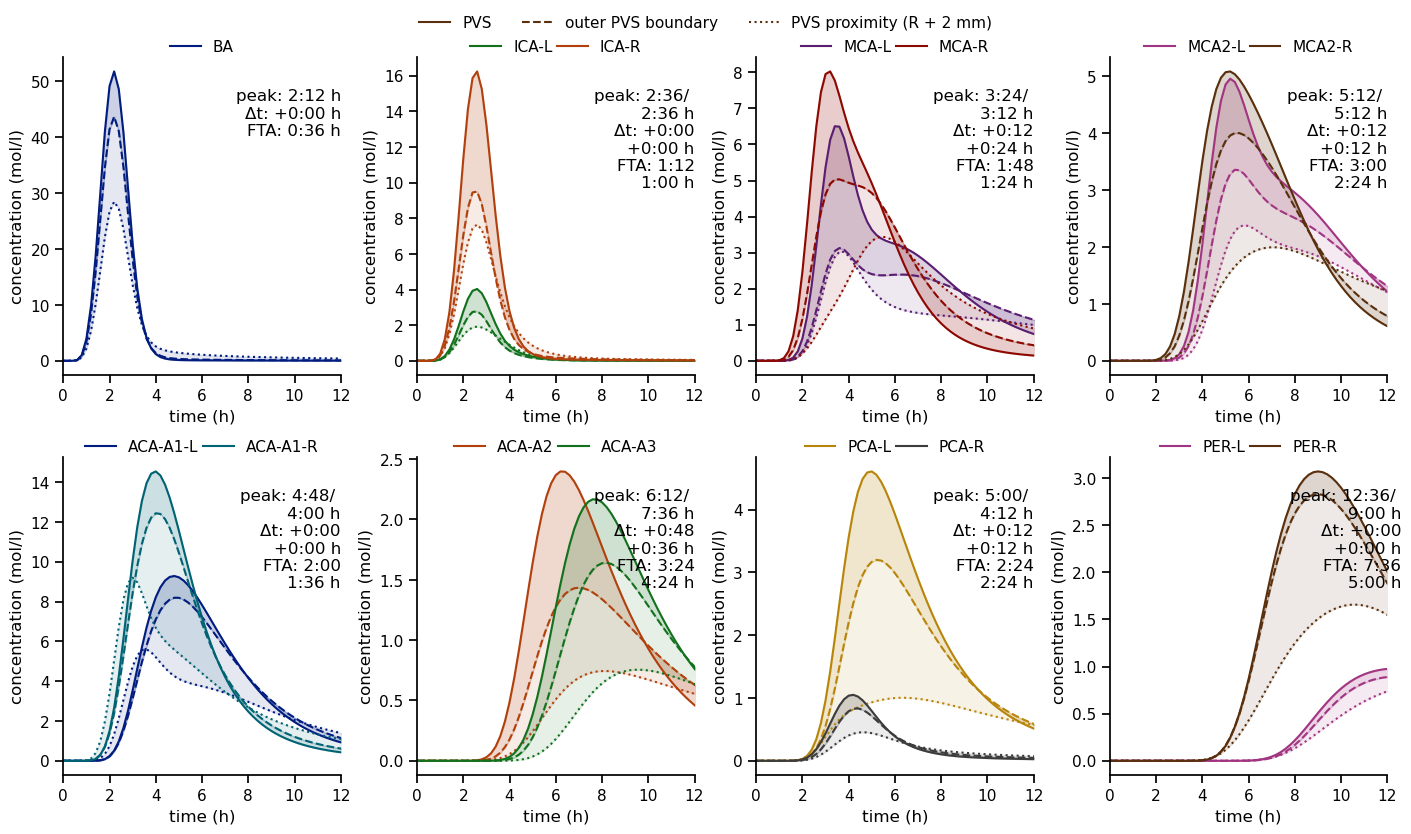
\includegraphics[width=1\linewidth]{figures/modelB2-10_conc_at_label.png}
    \caption{B2 - $10 \xi$}
    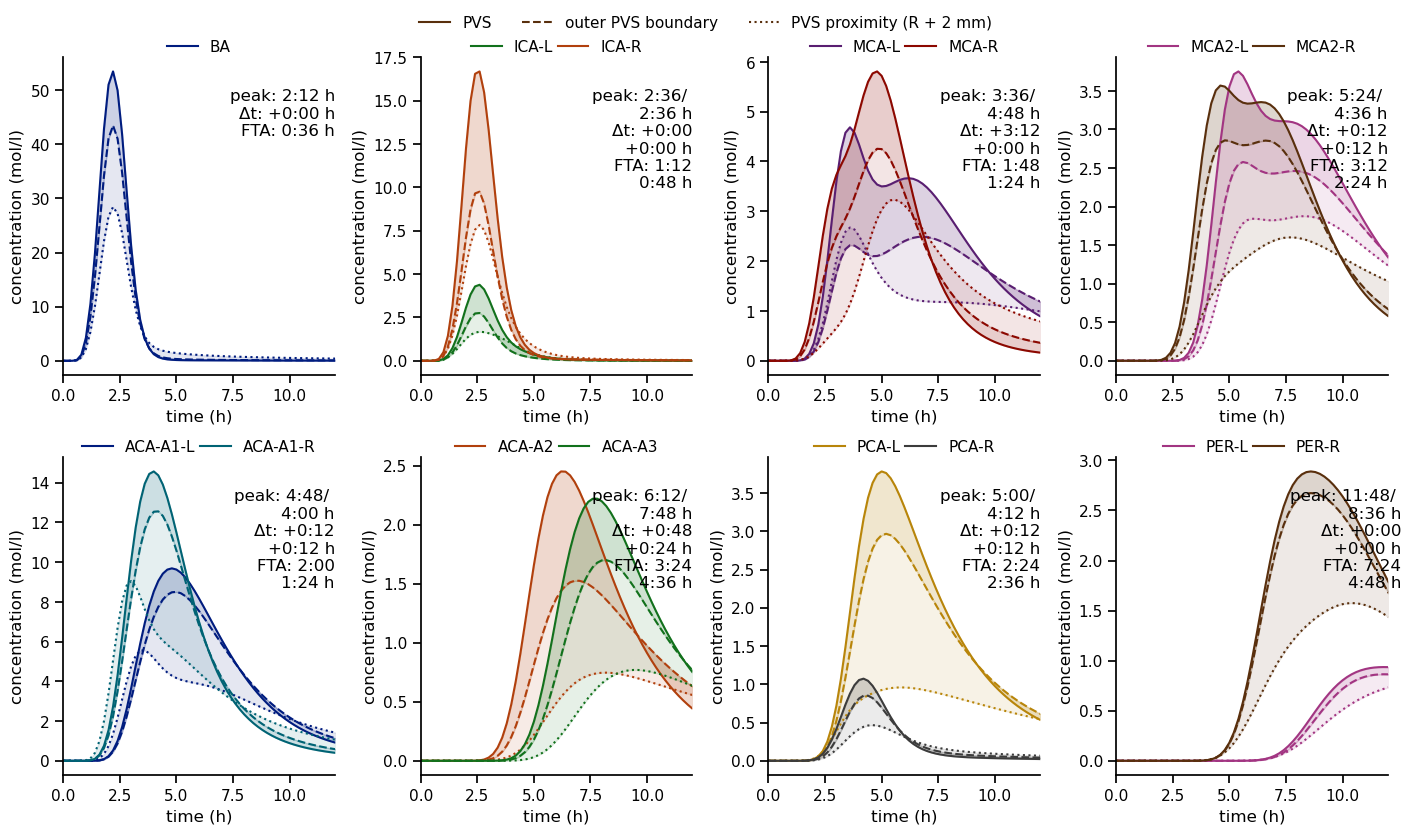
\includegraphics[width=1\linewidth]{figures/modelB2-100_conc_at_label.png}
    \caption{B2 - $100 \xi$}
    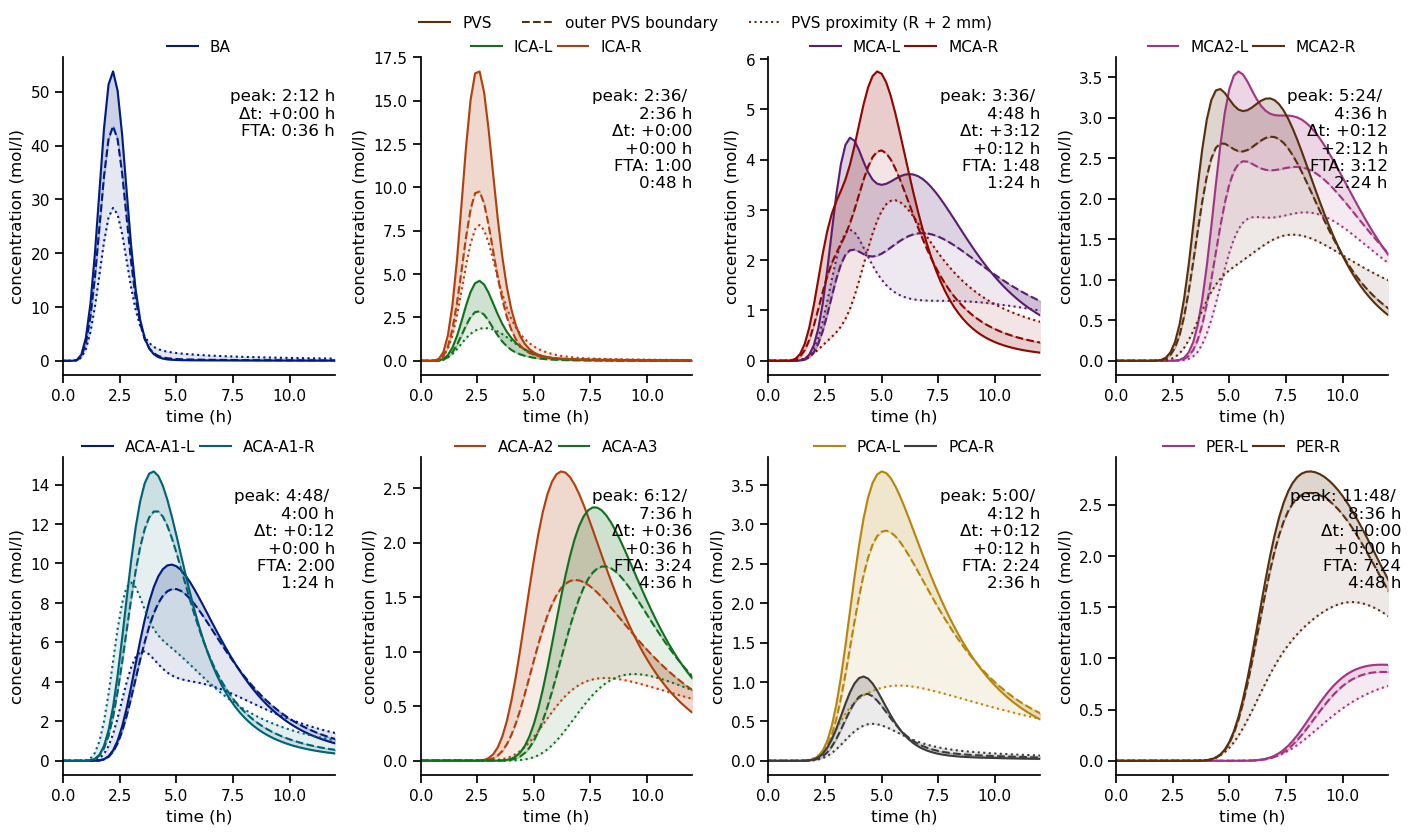
\includegraphics[width=1\linewidth]{figures/modelB2-1000_conc_at_label.png}
    \caption{B2 - $1000 \xi$}
\end{subfigure}
    \label{fig:modelB_xi_variations}
\end{figure}

\subsection*{The significance of low-resistance perivascular pathways}

\mer{MER: Remember to report on how much concentration enters into the brain?}
\begin{itemize}
\item
  Perivascular flow and transport has been identified as a key
  mechanism and potential target for enhancing brain drug delivery and
  metabolic waste clearance -- what are the global (intracranial)
  effects of such intracranial highways? 
\item
  Compare Model A and B (\Cref{tab:scenarios}).
\item
  Do solutes move from PVS to the SAS, or both along the PVS and along the SAS?
\end{itemize}


\subsection*{Clearance and the brain's waterscape}
\begin{itemize}
\item 
  Modelling metabolite clearance rather than solute influx (Model
  C). Consider several diffusion coefficients corresponding to
  gadubutrol, dextran, tau and amyloid-beta, otherwise identical flow
  set-ups.
\end{itemize}

\subsection*{Intracranial solute influx and clearance during sleep}

\begin{itemize}
\item
  Sleep is known to affect a number of the transport characteristics including: increased extracellular volume fraction, altered vascular pulsatility and a-forteriori perivascular flow and mixing, reduced CSF production, reduced glymphatic transport.
\end{itemize}


\subsection*{Influx and clearance in pathologies}
\begin{itemize}
\item
  A number of neurological and neurodegenerative disorders yield mechanical changes in the intracranial environment (increased arterial stiffness, cerebral arterial angiopathies, perivascular flow changes due to hypertension, altered CSF flow patterns, altered diffusion properties in cancer, BBB leakage). One key clinical aspect is increased PVS width in e.g. iNPH. 
\end{itemize}


\subsection*{Veins}
\mer{MER: Just a placeholder. Disregard veins in the first sections.}

\newpage

\mer{MER: Old, revisit to see if we have forgotten any of these interesting ideas.}
\subsection*{Effect of interfaces (interface permeability)}

\begin{itemize}
    \item Model 0 (baseline): only diffusion, different diffusion coefficient in the parenchyma and SAS/PVS. No leak to vasculature (zero permeability). $\infty$ $\zeta_0$ at the PVS-SAS interface, $\zeta_1$ at the PVS-SAS interface. Koch et al could be a reference for PVS-parenchyma, maybe Tithof et al (2022, "A network model" ...) could give some ideas for parameters, also see Mestre et al, Nature comms, 2022. 
    \item 
    With altered interface permeabilities in the PVS (Model 1), and or in the parenchyma (Model 2) 
    \end{itemize}


\subsection*{Effect of convection}
\begin{itemize}
    \item 
    With convective flow in the PVS (zero flow in the parenchyma for now)
    \begin{itemize}
        \item 
        Model 3: PVS flow equal to 18.7 $\mu$m/s
        \item 
        Model 4: Better PVS flow (distributed, according to conservation of mass, assumptions on PVS area)
    \end{itemize}    
    \item 
    With convective flow in the ECS (out of scope here, for follow-up work?)
\end{itemize}

\begin{figure}
    \centering
    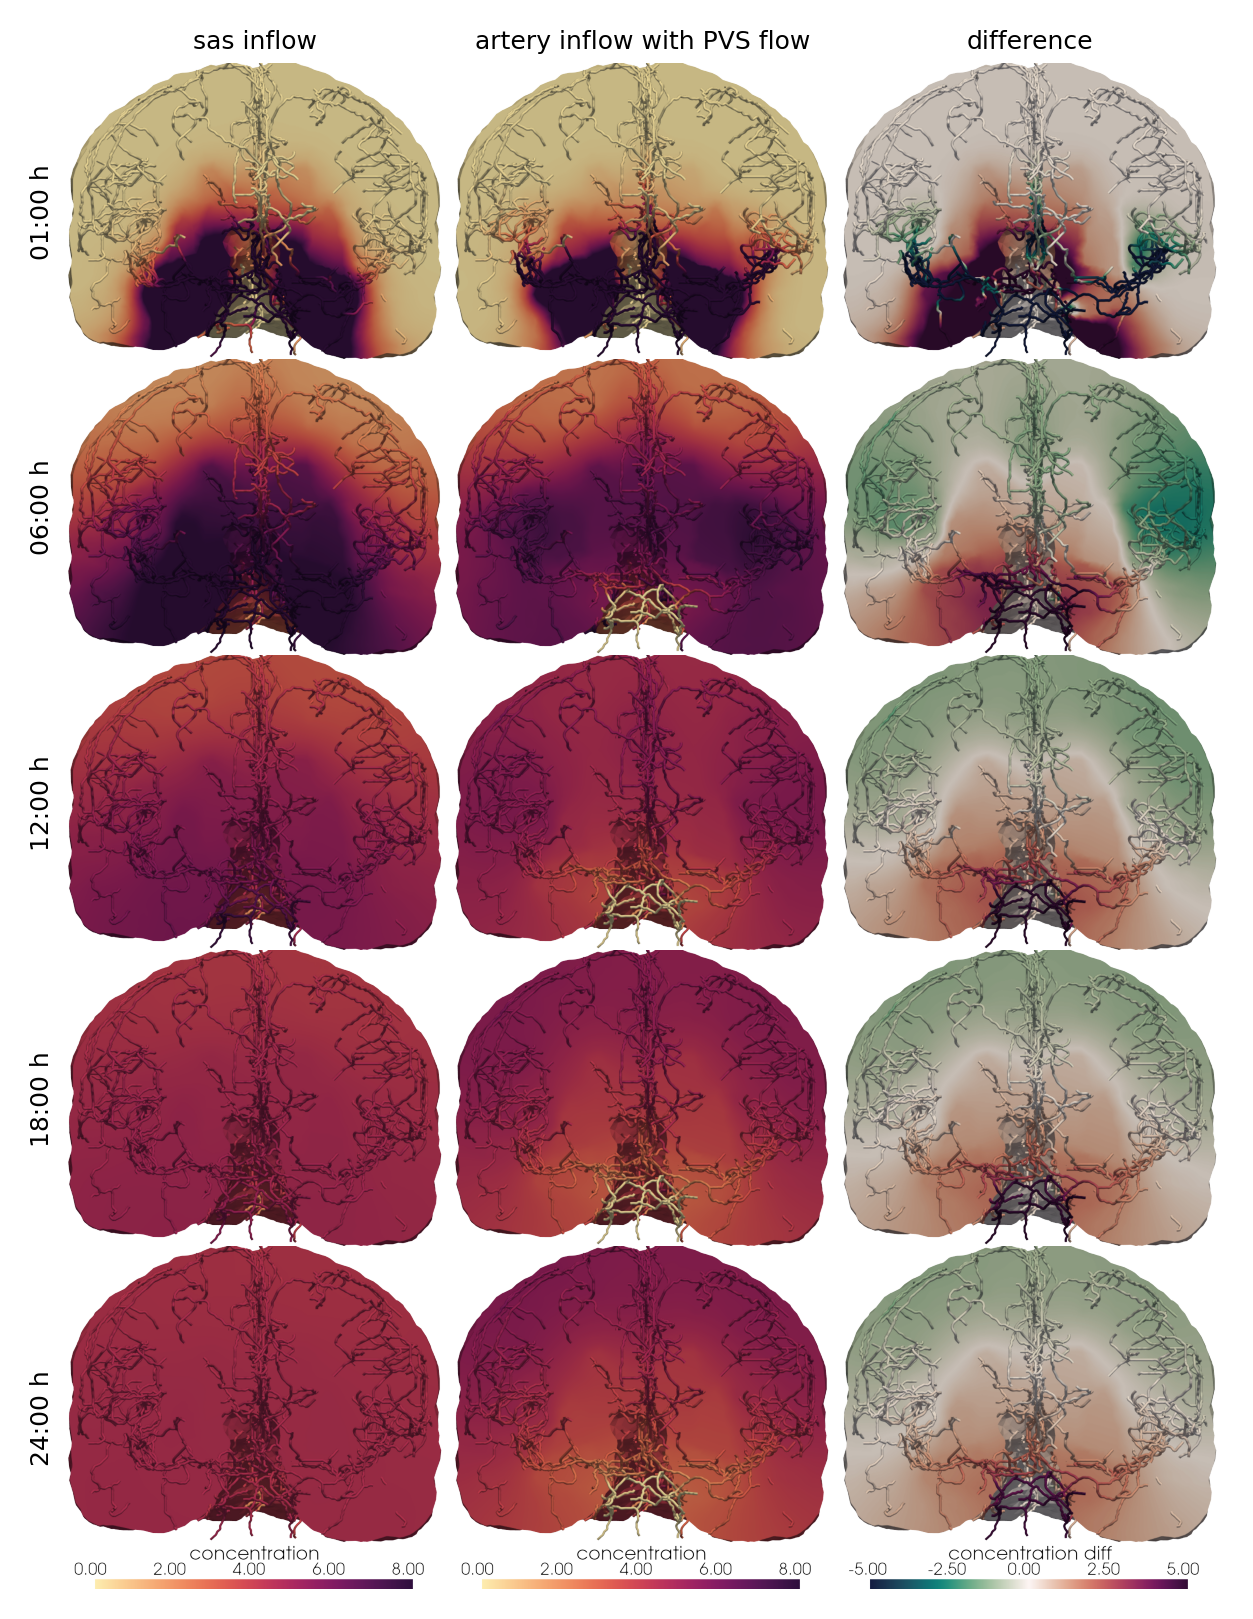
\includegraphics[width = 0.9 \textwidth]{modelB_modelC_overview.png}
    \caption{Tracer concentrations for a purely diffusive model with tracer inflow via the CSF-filled space (left) and a convective model with Tracer inflow via the arterial PVS (middle) and their difference (right) at 1, 6, 12, 18 and 24 hours after injection.}
    \label{fig:2}
\end{figure}
\subsection*{Effect of BBB}

Leakage to the blood, some sink/non-zero permeability for the PVS-blood (BBB) interface (Model N).

\subsection*{Effect of pia}
  
Effect of pia permeability (Model N-1)    

\begin{figure}
     \centering
     \begin{subfigure}[b]{0.33\textwidth}
         \centering
         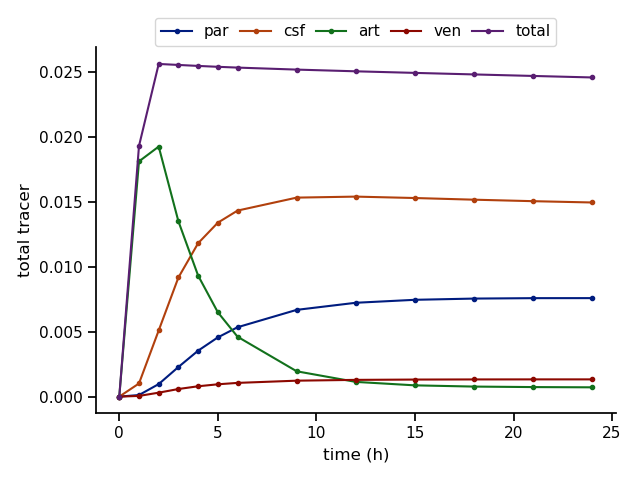
\includegraphics[width=\textwidth]{modelA_total_conc.png}
         \caption{arterial inflow, pure diffusion}
         \label{fig:y equals x}
     \end{subfigure}
     \hfill
     \begin{subfigure}[b]{0.33\textwidth}
         \centering
         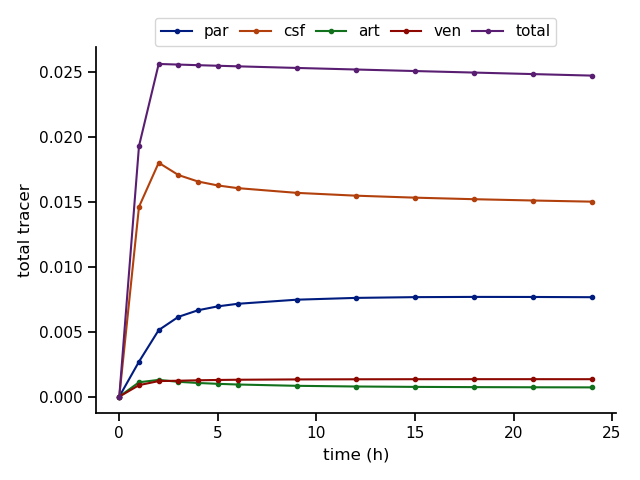
\includegraphics[width=\textwidth]{modelB_total_conc.png}
         \caption{SAS inflow, pure diffusion}
         \label{fig:three sin x}
     \end{subfigure}
     \hfill
     \begin{subfigure}[b]{0.33\textwidth}
         \centering
         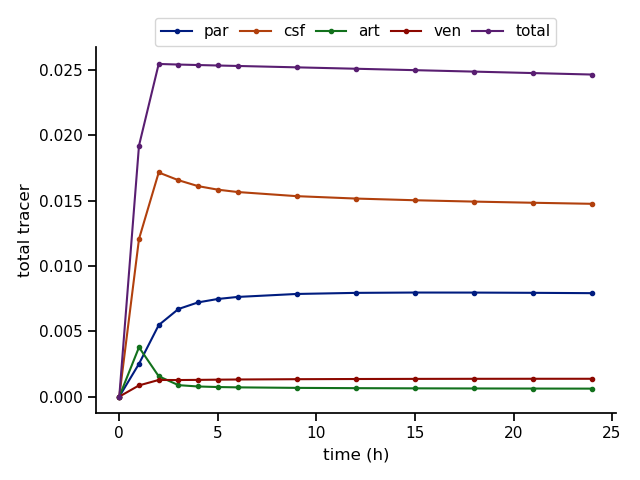
\includegraphics[width=\textwidth]{modelC_total_conc.png}
         \caption{arterial inflow, diffusion + PVS convection}
         \label{fig:five over x}
     \end{subfigure}
        \caption{Total tracer amount in parenchyma, CSF, arterial PVS and venous PVS}
        \label{fig:three graphs}
\end{figure}

\newpage
%%%%%%%%%%%%%%%%%%%%%%%%%%%%%%%%%%%%%%%%%%%%%%%%%%%%%%%%%%%%%%%%%%%%%%%%%%%%%%%%%%%%%
\section*{Methods}

%\mer{MER: I recommend writing each (sub)section of Methods as a nearly stand-alone paragraph. Let's see if we can avoid subsubsections/paragraphs. If you need to add more detail than you think is appropriate, put it in a Supplementary Methods section in the Appendix.} 

\subsection*{Intracranial compartments: ventricular system, SAS, and brain parenchyma}

From T1-weighted MR images of a human subject~\cite{hodneland2019new},
we first automatically segment the brain parenchyma and CSF spaces,
including the ventricular system and SAS, using
Synthseg~\cite{billot2023robust,billot2023synthseg}. We next manually
adjust the segmentation to accurately represent the connections
between CSF spaces (aqueduct, median aperture), smoothen, and finally
extract surface representations of the outer (arachnoid) boundary, the
pial membrane and other interfaces. Conforming to these surface and
interface representations, we generate a tetrahedral mesh $\Omega$
representing the complete intracranial volume as the union of the
parenchyma $\Omega_{\rm PAR}$ and CSF spaces $\Omega_{\rm CSF}$, using
fTetWild~\cite{hu2020fast}. The resulting computational mesh consists
of $153\,729$ vertices and $851\,904$ mesh cells, which vary between
$0.4$ mm and $1.2$ cm in mesh cell diameter. The parenchyma has a
total volume of $1386$ ml, whereas the ventricles and the outer SAS
contribute $28$ ml and $277$ ml, respectively, to a total CSF volume
of $305$ml, in agreement with recent
estimates~\cite{hladky2024regulation}.

%% In addition, we slightly modify the segmentation to ensure correct
%% connectivity of the ventricular system. In particular, we elongate
%% the aqueduct and enforce no communication between the ventricles
%% and the surrounding CSF spaces except for the median aperture.
%% After morphological smoothing of the segmented image, we extract
%% surface representations of the outer SAS boundary, the pial
%% membrane and the components of the ventricular system.

%% Note that the widely reported value of $150$\,ml of intracranial
%% CSF volume is likely an underestimate. Recent estimates indicate
%% that a value of $200$ to $300$\,ml is more accurate (see
%% \cite{hladky2024regulation} and references therein

\subsection*{Periarterial and perivenous spaces}

To represent surface networks of periarterial and perivenous spaces,
we use Kiminaro~\cite{william_silversmith_2021_5539913} to separately
skeletonize time-of-flight angiography (ToF) and quantitative
susceptibility mapping (QSM) images from the same human
subject~\cite{hodneland2019new}. This technique yields networks of
one-dimensional curves, each curve $\Lambda^i$ indicating the
centerline of a blood vessel segment and labeled with its lumen radius
$R_1^i$. We also assign an outer radius $R_2^i > R_1^i$ to each
segment $i$, form the annular cylinder ensheathing $\Lambda^i$ and
define the union of these as the PVS. The periarterial network graph
consists of $12\,708$ edges connected at $12\,562$ inner nodes and
with $147$ end nodes, and the associated domain is denoted by
$\Lambda_a$. We identify three of the end nodes -- corresponding to
the two internal carotid arteries (ICAs) and the basilar artery (BA)
-- as root nodes, and designate the other ends as leaf nodes. The
resulting perivenous network graph consists of $\fixme{N}$ edges
connected at $\fixme{N}$ inner nodes and with $\fixme{N}$ end nodes,
and the associated domain is denoted by $\Lambda_v$. \fixme{Finally, we label
the outer surface of the PVS associated with $\Lambda_a$ and
$\Lambda_v$, by $\Gamma_a$ and $\Gamma_v$ respectively.}

%% The resulting vascular networks are further smoothened using a
%% spline interpolation technique, and represented as graphs with
%% nodes connected by edges.

\subsection*{Molecular transport equations}

We model diffusion, convection, and exchange of a molecular solute in
the PVS networks $\Lambda_a$ and $\Lambda_v$, in the CSF spaces
$\Omega_{\rm CSF}$ and in the brain parenchyma $\Omega_{\rm PAR}$ via
a mixed-dimensional transport model~\cite{masri2023modelling} over a
timescale of minutes to hours. Specifically, for $t > 0$, we solve for
a concentration $c = c(x, t)$ in the 3D intracranial compartments ($x
\in \Omega_{\rm CSF}, x \in \Omega_{\rm PAR}$) and for a cross-section
averaged concentration $\hat{c} = \hat{c}(s, t)$ in the periarterial
and perivenous networks ($s \in \Lambda_a, s \in \Lambda_v$) such that
the following equations hold:
\begin{subequations}
\begin{alignat}{2}
  \partial_t (\phi c) - \nabla \cdot (D \nabla (\phi c) ) + \nabla \cdot (\bm u c ) + \xi (\overline{c} - \hat c ) \delta_\Gamma & = 0 && \quad \quad \mathrm{in} \quad \Omega_{\rm CSF}, \Omega_{\rm{PAR}},
  \label{eq:multi_transport_3d}
  \\ 
  \partial_t (A  \hat c) - \partial_s(\hat D A \partial_s ( \hat c)) +\partial_s(A \hat u \hat c )  +  \xi P (\hat c - \overline{c})  &= 0 && \quad \quad \mathrm{in} \quad  \Lambda_a, \Lambda_v .
  \label{eq:multi_transport_1d}
 \end{alignat}%
\label{eq:multi_transport}%
\end{subequations}%
In~\eqref{eq:multi_transport}, $0 < \phi \leqslant 1$ is the fluid
volume fraction, $D$ and $\hat{D}$ are effective diffusion
coefficients, and $\bm u$ and $\hat{u}$ are fluid (CSF/ISF)
velocities, all defined in the respective compartments; $P = 2 \pi
R_2$ is the perimeter and $A = \pi (R_2^2 - R_1^2)$ the area of the
PVS cross-sections, $\delta_{\Gamma}$ is the Dirac delta function
concentrated on the interfaces $\Gamma_a, \Gamma_v$, the overlined
$\overline{c}$ denotes the average of $c$ over cross-sections of
$\Gamma_a, \Gamma_v$, and $\xi$ is a permeability allowing for
transfer/exchange over the interfaces $\Gamma_a, \Gamma_v$ between the
periarterial and perivenous networks and their surroundings.
Moreover, we model the membrane between the parenchyma and the CSF
spaces as a semi-permeable membrane with permeability cofficient
$\beta_{\rm pia}$. For a complete description of this mathematical
model, see \Cref{sec:more_maths}.

\subsection*{Intracranial influx after intrathecal injection}
To represent molecular influx into the intracranial compartments
following intrathecal injection, without modelling the spinal
compartment explicitly, we prescribe a time-dependent molecular influx
over the interface towards the spinal compartment with the condition
$(D \nabla c - \bm u c ) \cdot \bm{n} = g_{\mathrm{influx}}$ on
$\Gamma_{\mathrm{SSAS}}$. We set
\begin{equation}
  g_\mathrm{influx}(t) = \frac{m_{\rm tot}}{T_{\rm max}^2 |\Gamma_{\rm SSAS}|} \max(0, T_{\rm max} - |t - T_{\rm max}|)
\end{equation}
which expresses a hat-shaped influx function with a peak at $T_{\rm max}$ and a total tracer injection of $m_{\rm tot}$ (\Cref{tab:parameters}).

\subsection*{Molecular clearance from the intracranial space and perivascular network ends}
%\subsection*{Boundary conditions: extracranial efflux and perivascular parenchymal influx}

We model molecular clearance, into the meningeal lymphatics or other
pathways, across the upper, outer (arachnoid) boundary
(\Cref{fig:intracranial_domains}), proportional to the concentration
in the SAS with a rate constant $\beta_{\rm exit}$. We set a no-flux
condition at the end nodes of the perivascular networks, not allowing
for direct molecular clearance there.

\subsection*{CSF flow in the SAS and ventricular system}
\label{sec:csf_fluid_vel}

We model CSF as an incompressible Newtonian fluid at low Reynolds and
Womersley numbers via the Stokes equations with viscosity $\mu$, and
account for the convective contribution of the flow induced by CSF
production in the choroid plexus. Specifically, we compute the
velocity $\bm u_{\rm CSF}$ and associated pressure $p_{\rm CSF}$ in
the SAS and ventricular system induced by a constant production at a
rate of $u_{\rm in}$ across the lateral ventricle walls and with
efflux across the upper, outer (arachnoid) boundary with efflux
resistance $R_0$; and then set $\bm u = \bm u_{\rm CSF}$ in
$\Omega_{\rm CSF}$ in~\eqref{eq:multi_transport}
(\Cref{tab:parameters}, \Cref{fig:intracranial_domains},
\Cref{fig:csf_flow_prod}, see also \Cref{sec:more_maths}). We do not
directly model convection within the brain tissue (beyond the
perivascular spaces), and thus set $\bm u = 0$ in $\Omega_{\rm PAR}$
in~\eqref{eq:multi_transport}.

\subsection*{Dispersion in the CSF spaces}

The pulsatile flow of CSF in the SAS and ventricular system,
associated with the cardiac and respiratory cycles, substantially
enhances molecular diffusion through
dispersion~\cite{taylor1953dispersion, watson1983diffusion,
  asgari2016glymphatic, keith2019dispersion, ray2021quantitative,
  troyetsky2021dispersion}. To account for these dispersive effects,
we compute a spatially-varying dispersion factor $R$ in $\Omega_{\rm
  CSF}$ (\Cref{fig:csf_flow_R}) by combining a computational model of
the CSF pressure gradient at peak arterial dilation with theoretical
estimates for shear-augmented (Taylor) dispersion
\cite{taylor1953dispersion, watson1983diffusion, keith2019dispersion}. \mer{Include 1-2 sentences from Supplementary Methods here -- but which? And also revisit references with MC.}

\mer{MER: Stopped here. WIP in Supplementary Methods.}

\subsection*{Dispersion in the PVS}

Similar to the CSF spaces, dispersion due to cardiac and respiratory pulsation has been hypothesized to enhance transport in the perivascular spaces. However, recent estimates indicate that the effect of dispersion does not exceed a factor of 2 compared to diffusion alone \cite{asgari2016glymphatic,keith2019dispersion,bojarskaite2023sleep,asgari2016glymphatic,troyetsky2021dispersion}, and we thus do not model dispersive effects in the PVS. 
\mar{Maybe we should just take a factor of 2 as the upper bound?}

% \cite{keith2019dispersion}: dispersion in PVS is negligiable in porous PVS, but might be relevant in open PVS (R=220) (theoretical estimates)
%  \cite{bojarskaite2023sleep} numerical simulations show that the enhancement factor is likely in the range of 10 - 50 \%
%\cite{asgari2016glymphatic} numerical simulations show increase of 16% to 50%  in distribution lengths
%\cite{troyetsky2021dispersion}:   maximum enhancement of diffusion of only about 5%




\subsection*{Perivascular fluid flow induced by CSF pressure differences}

Since the pressure gradient the caused by the steady production-driven CSF flow (see \cref{sec:csf_fluid_vel}), we impose the precomputed fluid pressure $p_{\rm CSF}$ on the networks root nodes:
\begin{equation}
    \hat{p} = p_{\rm CSF} \quad \text{ on } \Lambda^{\rm out}
\end{equation}
In case that the root does not lie within the CSF-space but the parenchyma, the CSF pressure is not yet computed. For that reason, we apply a simple extension technique to map the CSF pressure field into $\Omega_{\rm PAR}$. In particular, we solve a Laplace equation on $\Omega_{\rm PAR}$ with the CSF pressure on the Pial membrane ($\Gamma_{\rm Pia}$) as a boundary condition.


\subsection*{Perivascular fluid flow induced by vascular wall motion}

Using the theoretical framework introduced by Gjerde et
al.~\cite{gjerde2023directional}, we compute analytic estimates for
the time-average perivascular flow rate $\langle Q' \rangle$ induced
by rhythmic vascular wall motions for different frequencies $f$,
amplitudes $\varepsilon$ and wave lengths $\lambda$ in the arterial
network $\Lambda^a$ (see also Supplementary
Methods~\ref{sec:sup:peristalsis}). The corresponding contribution to
the convective velocity $\hat{u}_{\rm x}$ is defined vessel-wise as
$\hat{u}_{\rm x}|_{\Lambda_i} = \langle Q'_i \rangle/A_i$ where $A_i$
is the cross-section area of the PVS segment ($A_i = \pi (R_2^i -
R_1^i$)) and $\langle Q_i' \rangle$ is its mean flow rate. Two wall
motion patterns are considered: \emph{cardiac} pulsations with $f =
1.0$ (Hz), $\lambda = 2000$ (mm) and $\varepsilon = 1\%$, and very
low-frequency \emph{vasomotion} with $f = 0.1$ (Hz), $\lambda = 20$
(mm), and $\varepsilon = 10\%$. \mer{The corresponding net convective
velocities (in the antegrade direction) are for \emph{vasomotion}:
$9.345 \pm 6.695$ $\mu$m/s, range: $(-65.81, 63.96) \mu$m/s, and for
\emph{cardiac}: $0.475 \pm 0.5115 \mu$m/s, range: $(- 3.825, 4.861)
\mu$m/s, where negative velocities correspond to retrograde flow
(\Cref{fig:pvs}\mer{X}).} No perivascular fluid flow induced by wall
motion is considered for the venous network.


\subsection*{Model and material parameters}

Model and material parameters are summarized in \Cref{tab:parameters}.
We assume that the porosity equals the extracellular space volume
fraction $\phi = \phi_{\rm PAR}$ within the parenchyma and $\phi = 1$
elsewhere. In influx scenarios, we model the concentration of
Gadubutrol with effective diffusion coefficient equal to that of
Gadubutrol in free water in the PVS networks: $\hat{D} = D^{\rm Gad}$;
weighted by a dispersion factor $R$ in the CSF spaces:
$D|_{\Omega_{\rm CSF}} = ( 1 + R) D^{\rm Gad}$; and modulated by the
porosity and tortuousity ($\lambda = 1.78$) in the parenchyma:
$D|_{\Omega_{\rm PAR}} = D^{\rm Gad}_{\rm PAR}$. We set $\xi$
depending on whether the PVS segment is fully embedded within the CSF
spaces ($\xi = \xi_{\rm CSF}$) or parenchyma ($\xi = \xi_{\rm EF}$),
or neither (\Cref{sec:more_maths}). Additionally, we increase the
permeability $\xi$ ($100\times$) near the leaf nodes of $\Lambda_a$ to
account for the transition from explicitly resolved PVSs to their
unresolved continuation in the CSF spaces and parenchyma.

\begin{table}
  \begin{center}
    \begin{tabular}{ll|ccc}
      \toprule
      Parameter& Symbol & Value & Unit& Reference\\
      \midrule
      Extracellular space volume fraction & $\phi_{\rm PAR}$ & 0.2 & -- & \cite{nicholson1981ion} \\
      Free diffusion coefficient, Gadubutrol & $D^{\rm Gad}$ & $3.8 \times 10^{-4}$& $\text{mm}^2/\text{s}$ & \cite{valnes2020apparent}\\
      Parenchymal diffusion coefficient, Gadubutrol & $D^{\rm Gad}_{\rm PAR}$ & $1.2 \times 10^{-4}$ & $\text{mm}^2/\text{s}$  & \cite{hornkjol2022csf} \\
      Permeability coefficient, pia & $\beta_{\rm pia}$ & $2.6 \cdot 10^{-8}$ & m/s & \cite{riseth2025twocompartment} \\
      Permeability coefficient, endfoot sheath & $\xi_{\rm EF}$ & $3.8\cdot 10^{-7}$  & m/s & \cite{koch2023estimates} \\
      Molecular efflux rate & $\beta_{\rm exit}$ & $10^{-4}$ & mm$^2$/s & \cite{hornkjol2022csf} \\
      Total molecular volume & $m_{\rm tot}$ & $0.5$ & mmol & \cite{eide2024functional} \\
      Molecular influx, time-to-peak & $T_{\rm max}$ & $1$ & h & \fixme{$\ast$} \\
      CSF production rate & $u_{\mathrm{in}}$ & $0.63$  & l / day & \cite{nilsson1992circadian} \\
      CSF viscosity & $\mu$ & $0.7$ & mPa$ \cdot $s & \cite{bloomfield1998effects} \\ 
      CSF outflow resistance & $R_0$ & $10^{-5}$  & Pa/(mm$\cdot$s) & \cite{hornkjol2022csf} \\ 
      Dispersion factor, CSF spaces & $R$ & $\dagger$ & -- & $\ast$ \\
      \bottomrule
    \end{tabular}
  \end{center}
  \caption{Model parameters. $\dagger$/$\ast$ denotes computed/estimated within this work.}
  \label{tab:parameters}
\end{table}

\subsection*{Initial conditions}

We set the initial concentrations $c_0, \hat{c}_0$ in the
three-dimensional domain $\Omega$ and networks $\Lambda_a, \Lambda_v$
to be zero for all influx scenarios. For parenchymal
clearance scenarios, we set $c_0 = 1, \hat{c}_0 = 0$.

\subsection*{Numerical approximation of multi-dimensional transport and CSF flow}

\mer{@Rami: Could you draft one paragraph here describing the essential bits of the numerical scheme? I recommend ``describing with words'' to reach relevant audiences. Refer to the Supplementary Methods for details. Mention theoretical expected convergence order.} 

In this section, we provide a brief overview on the employed numerical discretization. We refer to \Cref{sec:details_numerical_method} for details. The numerical scheme for the CSF flow equations utilizes polynomial spaces that preserve the divergence free condition \eqref{eq:divergence_equation} on the discrete level \cite{hong2016robust}. This requirement is important for stability in the transport equation, see for example \cite{cesmelioglu2022compatible}. The spaces we used for the velocity are continuous along the normal direction; continuity of the tangential component is enforced via interior penalty approaches \cite{hong2016robust}.  If the exact solution of \eqref{eq:momnetum_equation}--\eqref{eq:divergence_equation} is smooth, then one expects optimal error convergence rates for this approximation. 

For the 3D transport problem, we use the interior penalty discontinuous Galerkin (DG) method with weighted averages and upwinding for the convection term \cite{ern2009discontinuous}.  We remark that the choice of DG in the 3D domain is necessary here since  continuous Galerkin methods even when supplemented with artificial diffusion stabilization terms were unstable in our experiments. For the 1D transport problem, we use continuous Galerkin spaces defined over the entire network with additional artificial diffusion silization when the 1D velocity is non--zero.  DG methods for the coupled 3D--1D problem have been recently analyzed  where convergence of the method for the elliptic case is established \cite{masri2024discontinuous}. While the analysis is for DG methods for both the 3D and the 1D problem, we expect similar arguments to hold here. However, note that the 3D--1D coupling induces a singularity in the 3D solution and one can only expect suboptimal error rates near the 1D network. In subdomains excluding the 1D lines, almost optimal rates can be expected for both DG methods \cite{masri2023discontinuous} and CG methods \cite{koppl2016local}.  Extension of the convergence analysis to convection--diffusion problems is an interesting future research direction. 
 


\begin{table}
  \begin{center}
  \begin{tabular}{ll|llllll|ll}
    \toprule
    & Description & $R_1, R_2$ & $\xi_{\rm PVS-SAS}$ &  $\beta_{\rm efflux}$ & $D$ & $\hat{u}$ & $\mathbf{u}_{SAS}$ & $c_0$ \\
    \midrule
    A & Baseline with sheaths & $R_2 = 2 R_1$ & $\xi$ & $10^{-4}$ mm$^2$/s\cite{hornkjol2022csf} & $\phi R D^{\rm gad}_{\rm eff}$\cite{sykova2008diffusion, valnes2020apparent} & $\hat{u}_{\rm prod} + \hat{u}_{\rm cardiac}$ & $\mathbf{u}_{\rm prod}$ & 0 \\ 
    B1 & Shealth permeability & $R_2 = 2 R_1$ & $0, \xi, 10 \xi, 100 \xi, 1000 \xi$ & $10^{-4}$ mm$^2$/s\cite{hornkjol2022csf} & $\phi R D^{\rm gad}_{\rm eff}$\cite{sykova2008diffusion, valnes2020apparent} & $\hat{u}_{\rm prod} + \hat{u}_{\rm cardiac}$ & $\mathbf{u}_{\rm prod}$ & 0 \\ 
    B2 & Shealth permeability & $R_2 = 2 R_1$ & $0, \xi, 10 \xi, 100 \xi, 1000 \xi$ & $10^{-4}$ mm$^2$/s\cite{hornkjol2022csf} & $\phi R D^{\rm gad}_{\rm eff}$\cite{sykova2008diffusion, valnes2020apparent} & $\hat{u}_{\rm prod} +  \hat{u}_{\rm cardiac} + \hat{u}_{\rm vaso}$ & $\mathbf{u}_{\rm prod}$ & 0 \\ 
    %C & Larger PVS & $R_2 = N R_1$ & -- & -- & --  &  --  & -- &  -- \\
    C & Higher PVS flow & -- & $\xi$ & -- & --  & $\hat{u}_{\rm prod} +  \hat{u}_{\rm cardiac} + \hat{u}_{\rm vaso}$  & -- & --  \\
    AA & PVS size & $R_2 = x \beta R_1$ & $\xi$ & -- & -- & -- &  -- & 0 \\ 
    %C & Larger PVS & $R_2 = N R_1$ & -- & -- & --  &  --  & -- &  -- \\
    B & PVS flow & -- & $\xi$ & -- & --  & $\hat{u}_{\rm prod} + \hat{u}_{\rm vaso}$  & -- & --  \\
    C & Clearance & -- & -- & -- & $\alpha D^{\rm gad, \tau, A\beta}$  & $\hat{u}_{\rm prod}$ & -- & 1 \\
    %E & PVS II & $R_2 = 2 R_1$ & $\xi$, -- & -- & --  &  $\hat{u} = \hat{u}_{\rm prod} + \uparrow\uparrow$  & -- & --  \\
    %F & PVS III & $R_2 = 2 R_1$ & $\xi$, -- & -- & $10 D_{\rm PVS}$ &  $\hat{u} = \hat{u}_{\rm prod}$  & -- & --  \\
    %G & Glymphatics & $R_2 = 2 R_1$ & $\xi$, -- & -- & \cite{sykova2008diffusion, valnes2020apparent} &  $\hat{u} = \hat{u}_{\rm prod} + \uparrow$  & $\mathbf{u}_{\rm PAR}$ > 0 & --  \\
    \bottomrule
    \end{tabular}
    \end{center}
  \caption{Overview of models (-- denotes as immediately above). Each
    PVS cross-section is modelled as a concentric annulus with inner
    radius $R_1$ and outer radius $R_2$ and such that $R_2 = \beta
    R_1$ with $\beta = 2.0$ based on~\cite{eide2024functional}. Let
    $\xi = \dots$ denote the permeability estimated by Koch et
    al.~\cite{koch2023estimates}. Model A and its variations aims to
    quantify the effect of PVS sheaths by varying the permeability
    $\xi$ between the PVS and its surroundings. We consider a fixed
    permeability $\xi_{\rm PVS-PAR}$ based
    on~\cite{koch2023estimates}. \mer{The permeability between the PVS
      and the SAS $\xi_{\rm PVS-SAS}$ must likely be estimated by a
      bit of trial-error from the observations of timings of PVS-SAS
      and SAS from~\cite{eide2024functional}.} \discuss{The
      extracranial solute efflux permeability $\beta_{\rm efflux}$ is
      uniformly distributed over the outer SAS boundary with a
      reasonable rate as baseline\cite{hornkjol2022csf,
        eide2021clinical, ringstad2024glymphatic}.} At baseline, the
    effective diffusion coefficients $D^{\rm x}_{\rm SAS} = D^{\rm
      x}_{\rm PVS}$ of the SAS and PVS represent the free diffusion
    coefficient of Gadubutrol (${\rm x} = {\rm gad}$) in CSF (water),
    and $D^{\rm x}_{\rm PAR}$ the effective diffusion coefficient of
    human cortical tissue, all at body temperature; weighted by a
    dispersion factor $\alpha$ (see Methods). At baseline, we consider
    net flow due to CSF-production in the SAS and PVS:
    $\mathbf{u}_{\rm SAS} > 0$ and $\hat{u} > 0$ (see Methods) but no
    bulk flow in the parenchyma $\mathbf{u}_{\rm PAR} = 0$. Due to the
    timescale for human intracranial tracer transport (minutes to
    hours) compared to typical (cardiac, respiratory, slow vasomotion)
    human intracranial pulsatility (0.1 -- 1 Hz), we consider net
    (constant-in-time) flow fields only in subsequent model variations
    (but see dispersion factor above).  Model B represents
    perivascular pathway scenarios with more rapid flow in the PVS
    induced by vasomotion (PVS I)~\cite{gjerde2023directional}.
    Models C represents a version of the aforementioned scenarios but
    for studying metabolite clearance (instead of solute influx).}
\label{tab:scenarios}
\end{table}


\mer{To be edited, just moved here:} We will consider different values for the SAS-PVS permeability $\xi$, including $\xi = 0$ (sealed PVS), $\xi \approx \infty$ (PVS continuous with SAS), as well as reasonable intermediate values. We will ignore PVS-blood exchange, and thus only model the perivascular concentration at the network level (in addition to the SAS/brain concentration in the surroundings).  

%%%%%%%%%%%%%%%%%%%%%%%%%%%%%%%%%%%%%%%%%%%%%%%%%%%%%%%%%%%%%%%%%%%%%%%%%%%%%%%%%%%%%
\newpage
\section*{Discussion}

\paragraph{CSF flow Model validation}

Hornkjøl et al \cite{hornkjol2022csf} model CSF flow induced by production in the choroid plexus and report a peak velocity of $8.9\,$mm/s in the aqueduct. Given that similar flow rates were enforced, the deviation from our value of $2.0\,$mm/s is likely due to differences in diameter of the reconstructed aqueduct. Additionally, their peak velocities in the SAS range between 20 - 50 $\mu\,$m/s, which is compatible with our mean velocity of $4.4\,\mu$m/s (\Cref{fig:csf_flow_histo}).

The aqueductal ($0.31\,$ml/s) and craniocervical ($8.31\,$ml/s) flow rates predicted by our model align well with previously reported values of $0.31\,$ml/s peak aqueductal flow rate \cite{vinje2019respiratory} and about $9\,$ml/s peak net blood inflow into the cranium \cite{baledent2014imaging}. Further, Linninger et al \cite{linninger2007cerebrospinal} model cardiac-induced CSF flow and predict a maximum transmantle pressure difference of $10\,$Pa, which is in good agreement with our estimate of $8.5\,$Pa as well as clinically measured mean pressure differences of $11.5\,$Pa between sensors placed subdurally and in the lateral ventricle \cite{vinje2019respiratory}.
% 10.7 cm/s CSF flow at the craniovertebral junction in control \cite{bapuraj2016cerebrospinal}, area difference?

Sharp et al used the theory of dispersive mixing to predict a dispersion enhancement factor of $91.8$ in the (open) spinal SAS, which lies well within the range of our spatially varying estimate (ranging from 0 to 160). Conversely, \cite{ray2021quantitative} report up to 10,000 times greater diffusion in perivascular regions, but their modelling lumps diffusive, dispersive and advective transport in a single enhancement factor and is thus not directly comparable.



\subsection*{Limitations}

\begin{itemize}
\item
  \mer{MER/MC: How about dispersion in the PVS?}
\item 
  Inaccuracies in vascular geometry representation - and consequences downstream for e.g. numerical integration.
\item
  PVS geometry assumptions and approximations. Humans different from mice. Limitations in resolution.
\item
  No vasculature in the cerebellum, and of course no vasculature below certain resolution.
\item
  Only partially accounting for pulsatility. Ignoring respiration frequencies - dubious in the context of CSF flow.
\item
  Accounting for brain diffusive anisotropy. Little effect expected. Maybe something to consider in small follow-up work.
\item
  Permeability and stiffness of the pial membrane
\item
  PVS-blood exchange and BBB leakage. Natural to consider in model variation here, or follow-up work.
\end{itemize}

\subsection*{Outlook}

\begin{itemize}
\item
  Considering the (maybe) low diffusion in CSF spaces, maybe pure
  advection would be relevant? Both computational and physiological
  implications/interest.
\end{itemize}

\bibliography{references}

\newpage
\section*{Acknowledgments (not compulsory)}

Acknowledgments should be brief, and should not include thanks to anonymous referees and editors, or effusive comments. Grant or contribution numbers may be acknowledged.

\section*{Author contributions statement}

Must include all authors, identified by initials, for example:
A.A. conceived the experiment(s),  A.A. and B.A. conducted the experiment(s), C.A. and D.A. analysed the results.  All authors reviewed the manuscript. 

\section*{Additional information}

To include, in this order: \textbf{Accession codes} (where applicable); \textbf{Competing interests} (mandatory statement). 

The corresponding author is responsible for submitting a \href{http://www.nature.com/srep/policies/index.html#competing}{competing interests statement} on behalf of all authors of the paper. This statement must be included in the submitted article file.

\newpage
\appendix
\section{Supplementary methods}

These sections provide more detailed descriptions of the mathematical models and numerical approximations considered.

\subsection{Mixed-dimensional transport and flow equations}
\label{sec:app:more_maths}

\subsubsection{Notation}

In terms of geometrical domains, we consider the parenchyma
$\Omega_{\rm PAR} \subset \R^3$ and CSF spaces $\Omega_{\rm CSF}
\subset \R^3$ with $\Omega = \Omega_{\rm PAR} \cup \Omega_{\rm CSF}$
(\Cref{fig:results1}A, \Cref{fig:csf}A--C). The coordinates in these
3D domains is denoted by $x$. The interface between the parenchyma and
CSF spaces is given by $\partial \Omega_{\rm PAR} \cap \partial
\Omega_{\rm CSF}$ and we separate it as two parts: the surface of the
lateral ventricles $\Gamma_{\rm LV}$ and the remaining pial interface
$\Gamma_{\rm pia}$ (thus $\partial \Omega_{\rm CSF} \bigcap \partial
\Omega_{\rm PAR} = \Gamma_{\rm LV} \cup \Gamma_{\rm pia}$). The
remaining, outer, boundary of $\Omega_{\rm CSF}$ is again separated
into two parts: $\Gamma_{\rm SSAS}$ represents the lower interface
towards the spinal subarachnoid space (SSAS), while $\Gamma_{\rm AM}$
is the outer interface towards the arachnoid and dura
membranes. $\Gamma_{\rm AM}$ is further subdivided into its lower and
upper parts: $\Gamma_{\rm AM-L}$ and $\Gamma_{\rm AM-U}$. The boundary
towards the spinal cord is denoted by $\Gamma_{\rm{SC}}$ and given by
$\Gamma_{\rm{SC}} = \partial \Omega_{\rm PAR} \setminus \partial
\Omega_{\rm CSF}$.

In addition, we consider two sets of perivascular networks: a
periarterial network $\Lambda_a$ represented by the (connected)
centerlines $\Lambda^i_{a}$ of the arterial tree, and a perivenous
network $\Lambda_v$ associated with the centerlines $\Lambda^i_{v}$
of the veins. Recall that we represent the vascular domains as the
union of cylindrical vessels of radius $R_1^i$ surrounding the
centerlines $\Lambda^i$. Moreover, we consider the surrounding
perivascular spaces as the union of annular cylinders $\Omega^i$ of
inner radius $R_1^i$ and outer radius $R_2^i > R_1^i$ and thus of
width $R_2^i - R_1^i$, and remark that we interpret $R^i_2$ and $R^i_1$ as temporal averages (fixed in time), as the pulsations considered in \Cref{sec:app:peristalsis} are beyond the temporal resolution of our model. We denote the outer lateral surface of the
periarterial and perivenous spaces by $\Gamma_a$ and $\Gamma_v$,
respectively. We omit the subscript $a$ or $v$ when referring to any
such network, vessel segment or perivascular outer surface. We assume
that $\Lambda$ is parametrized by the coordinate $s$, and with a minor
abuse of notation, simply write $s \in \Lambda$ to represent the point
${\bm \lambda}(s)$ on $\Lambda$ corresponding to $s$. Finally, we view
each perivascular network both as a geometric domain and as a directed
graph with the centerlines $\{ \Lambda^i \}$ as oriented edges and the
connections as nodes $\mathcal{V}$.

\subsubsection{Solute transport and exchange in intracranial domains (3D) and perivascular networks (1D)}
\label{sec:app:transport_eqs}

In this section, we describe the mathematical
model~\eqref{eq:multi_transport}, the associated definitions,
interface and boundary conditions in further detail. We refer to the
main text for explicit parameter values while giving the general,
abstract form here, and to the reference~\cite{masri2024modelling, laurino2019derivation} for
the derivation and analysis of this 3D-1D model. Recall that we model
a concentration field $c = c(x, t)$ for $x \in \Omega$ and $t > 0$
defined in $\Omega_{\rm PAR}$ and $\Omega_{\rm CSF}$ separately. In
each of these domains, $c$ satisfies
%\mer{MER: Rami asks if it should be a $\phi$ in the advective term here. We can include it, or drop it, but in the latter case, perhaps we should clarify that u is an average/superficial/Darcy velocity.}
\begin{equation}
  \partial_t (\phi c) - \nabla \cdot (D \nabla (\phi c) ) + \nabla \cdot (\bm u c ) + \xi (\overline{c} - \hat c ) \delta_\Gamma
  %= f
   = 0
  \quad \quad \mathrm{in} \quad \Omega_{\rm CSF}, \Omega_{\rm{PAR}}.
  \label{eq:3d_pde}
\end{equation}
In~\eqref{eq:3d_pde}, $\phi$ is the fluid volume fraction (also known as the porosity) defined in the parenchyma ($\phi \ll 1$ in $\Omega_{\rm PAR}$) and in the CSF spaces ($\phi = 1$ in $\Omega_{\rm CSF}$). In the parenchyma, $\phi$ represents the extracellular space volume fraction, and thus $c$ here generally represents the intrinsic (in contrast to the superficial) concentration~\cite{sykova2008diffusion}. Moreover, $D$ is the effective diffusion coefficient of the relevant solute in the respective media which takes different values over the CSF spaces and the parenchyma, depending on tortuosity~\cite{sykova2008diffusion} and dispersive effects; and $\bm u$ is a convective velocity field representing the flow of CSF in $\Omega_{\rm CSF}$ and the flow of ISF in $\Omega_{\rm PAR}$. $\xi$ models a transfer or exchange parameter between the 3D domain ($\Omega_{\rm PAR}$ or $\Omega_{\rm CSF}$) and the perivascular networks $\Lambda_a, \Lambda_v$. To summarize,
\begin{equation*}
\phi =  \begin{cases}
  1  & \mathrm{in} \;  \Omega_{\rm{CSF}} \\ 
  \phi_{\rm{PAR}} & \mathrm{in} \; \Omega_{\rm{PAR}} 
  \end{cases}, \; 
D = \begin{cases}
  D_{\rm{CSF}} & \mathrm{in} \;  \Omega_{\rm{CSF}} \\ 
  D_{\rm{PAR}} & \mathrm{in} \; \Omega_{\rm{PAR}} \end{cases}, \; 
  \quad \bm u  = \begin{cases}
  \bm{u}_{\rm{CSF}} & \mathrm{in} \; \Omega_{\rm{CSF}} \\ 
  \bm{u}_{\rm{PAR}} & \mathrm{in} \; \Omega_{\rm{PAR}} 
\end{cases}, \; 
\xi = \begin{cases}
  \xi_{\rm{CSF}} & \mathrm{if} |\Omega^i \cap \Omega_{\rm{CSF}}| \neq 0 \\
  \xi_{\rm{EF}} & \mathrm{if} |\Omega^i \cap \Omega_{\rm{PAR}}| \neq 0  
\end{cases} . 
\end{equation*}
In the above, $\xi$ is defined segment-wise: for each centerline $\Lambda^i$ with surrounding PVS $\Omega^i$, $|\Omega^i \cap \Omega_{\rm{PAR}}|$ (resp. $|\Omega^i \cap \Omega_{\rm{CSF}}|$) is nonzero whenever $\Omega^i$ intersects $\Omega_{\rm{PAR}}$ (resp. $\Omega_{\rm{CSF}}$). If the surrounding PVS intersects both, then we set $\xi = \xi_{\rm EF}$ if $\Omega^i$ mainly ($80$ percent) intersects $\Omega_{\rm{PAR}}$, in which case the interaction with $\Omega_{\rm{CSF}}$ is ignored; otherwise, we set $\xi = \xi_{\rm CSF}$. 
 
Also in~\eqref{eq:3d_pde}, the notation $\overline{c}$ denotes a lateral average of the concentration over the outer perivascular surfaces, defined for each centerline $\Lambda^i$ and each point $s \in \Lambda^i$ by
\begin{equation*}
  \overline{c}(s) = \frac{1}{P(s)} \int_{\partial \Theta_2^i(s)} c 
\end{equation*}
where $\partial \Theta_2^i(s)$ is the outer boundary of the cross-section $\Theta(s)$ of the PVS $\Omega^i$ at $s$ and $P(s)$ is the perimeter of $\Theta(s)$. Moreover, for both the periarterial and perivenous networks ($\Lambda_a, \Lambda_v$ with outer PVS boundaries $\Gamma_a, \Gamma_v$), the term $\delta_\Gamma$ is concentrated on the outer lateral surfaces of the PVSs, and defined in terms of its action on any sufficiently smooth function $v : \Omega \rightarrow \R$
%and for each $\Lambda^i \subseteq \Lambda$ with PVS $\Omega^i$ and outer lateral surface $\Gamma^i = \partial \Omega^i_2$
such that
\begin{equation*}
  \langle \xi (\overline{c} - \hat c ) \delta_\Gamma, v \rangle =
  \int_{\Lambda} P \xi (\overline{c} - \hat c ) \overline{v}, 
\end{equation*}
under the assumption that $\xi$ is constant on each $\partial
\Theta_2^i$.
%% , since:
%% \begin{multline}
%%   \int_{\Omega} \xi (\overline{c} - \hat c ) \delta_\Gamma (v) =
%%   \int_{\Gamma} \xi (\overline{c} - \hat c ) \delta_\Gamma (v) =
%%   \sum_i \int_{\Gamma^i} \xi (\overline{c} - \hat c ) \delta_\Gamma (v) = 
%%   \sum_i \int_{\Lambda^i} \int_{\partial \Theta_2^i} \xi (\overline{c} - \hat c ) \delta_\Gamma (v) = \\
%%   \sum_i \int_{\Lambda^i} \left (  \xi (\overline{c} - \hat c ) \int_{\partial \Theta_2^i} \delta_\Gamma (v) \right ) =
%%   \sum_i \int_{\Lambda^i} P \xi (\overline{c} - \hat c ) \overline{v} =
%%   \int_{\Lambda} P \xi (\overline{c} - \hat c ) \overline{v} .
%% \end{multline}
%% \mer{MER: The previous was:
%% \begin{equation}
%%   \xi (\overline{c} - \hat c ) \delta_\Gamma (v) = \int_{\Lambda} P \xi ( \overline{c} - \hat c ) \overline{v} .
%% \end{equation}
%% }

On the interface between the brain and the CSF spaces
$\Gamma_{\mathrm{pia}} \cup \Gamma_{\rm LV}$, we prescribe the
following interface conditions, which represent a semi--permeable
interface, writing $c|_{\Omega_{\rm PAR}} = c_{\rm PAR}$ and
$c|_{\Omega_{\rm CSF}} = c_{\rm CSF}$:
%% \begin{subequations}
%% \begin{alignat}{2}
%% (-D \nabla (\phi c_{\rm{PAR}}) + \bm u_{\rm{PAR}} c_{\rm{PAR} }) \cdot \bm{n} &= - (- D (\phi \nabla c_{\rm{CSF}}) + \bm u_{\rm{CSF}} c_{\rm{CSF}} ) \cdot \bm{n} &&  \quad  \mathrm{on} \quad \Gamma_{\rm pia} \cup \Gamma_{\mathrm{LV}} ,  \\  
%% (-D \nabla ( c_{\rm{PAR}}) + \bm u_{\rm{PAR}} c_{\rm{PAR} }) \cdot \bm{n} & = \beta_{\rm{pia}} (c_{\rm PAR} - c_{\mathrm{CSF}}) &&  \quad  \mathrm{on} \quad \Gamma_{\rm pia} \cup \Gamma_{\mathrm{LV}} ,  
%% \end{alignat} 
%% \end{subequations}
\begin{subequations}
  \begin{alignat}{2}
  (-D \nabla (\phi c) + \bm u c)|_{\Omega_{\rm PAR}} \cdot \bm{n}
  &= - (-D \nabla (\phi c) + \bm u c)|_{\Omega_{\rm CSF}} \cdot \bm{n}
  &&  \quad  \mathrm{on} \quad \Gamma_{\rm pia} \cup \Gamma_{\mathrm{LV}} ,  \\  
  (- D \nabla (\phi  c) + \bm u c)|_{\Omega_{\rm PAR}} \cdot \bm{n} & = \beta_{\rm{pia}} (c_{\rm PAR} - c_{\mathrm{CSF}}) &&  \quad  \mathrm{on} \quad \Gamma_{\rm pia} \cup \Gamma_{\mathrm{LV}} ,  
\end{alignat} 
  \label{eq:3d_interface}%
\end{subequations}%
where $\bm{n} = \bm{n}_{\rm PAR}$ is the normal vector field defined
over the interface, outward-pointing when viewed from $\Omega_{\rm
  PAR}$, and $\beta_{\mathrm{pia}} \geqslant 0$ is a permeability
constant.

We supplement~\eqref{eq:3d_pde} and~\eqref{eq:3d_interface} with the following boundary conditions representing a given molecular influx at $\Gamma_{\rm SSAS}$, molecular efflux at a constant update rate $\beta_{\rm exit}$ at $\Gamma_{\rm AM-U}$, and no influx or efflux elsewhere from the CSF spaces.
\begin{subequations}
\begin{alignat}{2}
(D \nabla (\phi c) - \bm u c ) \cdot \bm{n} &= g_{\mathrm{influx}} &&  \quad  \mathrm{on} \quad \Gamma_{\rm SSAS},  \\ 
% (-D \nabla (\phi c) + \bm u c ) \cdot \bm{n}_{\Gamma_{\rm SAS}} &= 0 &&  \quad  \mathrm{on} \quad \Gamma_{\rm SAS}^{\mathrm{out}}  \\ 
(-D \nabla (\phi c) + \bm u c ) \cdot \bm{n} & = \beta_{\rm exit} c  &&  \quad  \mathrm{on} \quad \Gamma_{\rm AM-U},  \\ 
(-D \nabla (\phi c) + \bm u c ) \cdot \bm{n} & = 0  &&  \quad  \mathrm{on} \quad \Gamma_{\rm AM-L} \cup \Gamma_{\rm SC}  .
\end{alignat} 
\label{eq:3d_bcs}
\end{subequations}
where again $\bm n$ denotes the outward-pointing boundary normal.

The concentration $\hat{c} = \hat{c}(s, t)$ in the periarterial and
perivenous networks ($s \in \Lambda_a, s \in \Lambda_v$), entering
in~\eqref{eq:3d_pde}, represents the concentration in the perivascular
space averaged over each perivascular cross-section and is governed by 
\begin{equation}
  \partial_t (A  \hat c) - \partial_s( \hat D A \partial_s \hat c  ) + \partial_s(A \hat u \hat c )  +  \xi P (\hat c - \overline{c}) = 0
  \qquad \text{in} \quad \Lambda_a, \Lambda_v ,
\label{eq:1d_pde}
\end{equation}
where in $\Lambda_a, \Lambda_v$ refers to in each $\Lambda^i$ in each
of these networks. In~\eqref{eq:1d_pde}, $A = A(s)$ is defined as the
PVS cross-sectional area; i.e.,~for each $s \in \Lambda^i$ with
associated PVS $\Omega^i$, the area of the cross-section
$\Theta^i(s)$. Also, $\hat{D}$ is the effective diffusion coefficient,
and $\hat{u}$ is a convective velocity representing an (average) CSF
flow velocity in the axial direction of the perivascular spaces.

To complete~\eqref{eq:1d_pde}, we prescribe bifurcation conditions at
internal nodes of the perivascular networks $\Lambda_a, \Lambda_v$ and
boundary conditions at the end nodes. To this end, define the set of
internal nodes $\mathcal{B} \subset \mathcal{V}$ as the set of nodes
that are connected to two or more edges and the set of end nodes as
$\mathcal{N} \subset \mathcal{V}$, write $\hat{c}^i =
\hat{c}|_{\Lambda^i}$, and for $y\in\mathcal{B}$ let $\mathcal{E}(y)$ denote the set of
(two or three) edges in $\{\Lambda^i\}$ sharing the node $y$. To
impose continuity of the concentrations, we set that the
concentrations when viewed from each edge must match at nodes:
\begin{equation}
  \hat{c}^i (y) = \hat{c}^j(y)
  \qquad \foralls \Lambda^i, \Lambda^j \in \mathcal{E}(y)
  \qquad \foralls y \in \mathcal{B} .
  \label{eq:conc_continuity}
\end{equation}
Moreover, to ensure mass conservation, we set that the flux
going in and out at nodes should add to zero, or more precisely, that
for each $y \in \mathcal{B}$:
\begin{equation}
  \sum_{\Lambda^i \in \mathcal{E}(y)}
  \left (\hat{D}^i A^i \partial_s \hat{c}^i (y) - A^i \hat u^i(y) \hat{c}^i(y) \right ) n^i(y)
  = 0.
  \label{eq:flux_conservation}
\end{equation}
Here the (normal ``vector") function $n^i$ takes the values in $\left\{-1, 1\right\}$ and 
defines an orientation of vertices of edge $\Lambda^i$. Specifically, for an edge $\Lambda^i$ oriented from $y_{\rm in}$ to $y_{\rm out}$ we set 
\begin{equation}
  n^i(y_{\rm in}) = 1,\quad
  n^i(y_{\rm{out}}) = -1. %\quad
  %\mk{n^i(y) = 0 \quad \foralls y \in 
  %\mathcal{V} \backslash \{ y_{\rm in}, y_{\rm out} \} }.  
\label{eq:def:sign}
\end{equation}
%\mk{Why do we need the normal on non-IO vertices?}

Finally, we impose a homogeneous Neumann condition at all network end
nodes to augment~\eqref{eq:1d_pde}:
\begin{equation}
    \hat D A \partial_s (\phi \hat c) - A \hat u \hat c  = 0 \quad \mathrm{on} \quad \mathcal{N}.
    \label{eq:1d_bcs}
\end{equation}
This no-flux condition states that the network end nodes represent
barriers for molecular efflux into or out of the perivascular network,
and thus that all solute exchange between the PVSs and their
surroundings takes place via the lateral outer PVS surface and is
regulated by the exchange parameter $\xi$ cf.~\eqref{eq:3d_pde}
and~\eqref{eq:1d_pde}. Larger particles have been observed to
accumulate within the PVS as the surface arteries penetrate into the
brain parenchyma~\cite{mestre2018flow, bedussi2018paravascular},
and~\eqref{eq:1d_bcs} is appropriate to represent such
behavior. However, to represent a continuously extending PVSs also
along penetrating vessels, this condition should be revisited.

\subsubsection{Modelling CSF flow via the incompressible Stokes equations}
\label{sec:app:csf_flow}
The time-independent, incompressible Stokes equations model the flow
of an incompressible Newtonian fluid at low Reynolds numbers, and read
as follows: over the domain $\Omega_{\rm CSF} \subset \R^3$, find the
velocity vector field $\bm u : \Omega_{\rm CSF} \rightarrow \R^3$ and
the pressure field $p : \Omega_{\rm CSF} \rightarrow \R$ such that
\begin{subequations}
  \begin{alignat}{2}
    - \mu \Delta \bm u  + \nabla p &=  0 \quad && \text{ in } \Omega_{\rm CSF},
    \label{eq:momentum_equation} \\ 
    \nabla \cdot \bm u &= 0 \quad && \text{ in } \Omega_{\rm CSF}
    \label{eq:divergence_equation} .
  \end{alignat}
  \label{eq:stokes}%
\end{subequations}%
In addition, we impose the following boundary conditions to model flow
induced by CSF production in the choroid plexus with $\Gamma_{\rm AM-U}$ as the main efflux site:
\begin{subequations}
  \begin{alignat}{2}
( \mu \nabla \bm u \cdot \bm{n} - p \bm n) \cdot \bm n  &= -R_0 ( \bm u \cdot \bm n ), \quad \bm u \cdot \bm t = 0
    && \text{ on } \Gamma_{\mathrm{AM-U}}, \\
    \bm u &= 0 && \text{ on } \Gamma_{\mathrm{AM-L}}\cup\Gamma_{\rm{pia}}\cup\Gamma_{\rm{SSAS}}, \\
    %\bm u &= 0 && \text{ on } \Gamma_{\rm{pia}}, \\
    %\bm u &= 0 && \text{ on } \Gamma_{\rm{SSAS}}, \\
    \bm u \cdot \bm n & = \frac{1}{ |\Gamma_{\rm LV}|}  u_{\rm in}, \quad \bm u \cdot \bm t = 0 \quad && \text{ on } \Gamma_{\rm{LV}} ,  
  \end{alignat}
  \label{eq:stokes_bcs}%
\end{subequations}%
where $\bm n$ and $\bm t$ denote the unit outward normal and tangent vectors to the boundary respectively,  $\mu$ is the (dynamic) CSF viscosity, $R_0 > 0$ is a resistance parameter for CSF efflux, and $u_{\rm in}$ is a given fluid influx, here across the lateral ventricle wall $\Gamma_{\rm LV}$. We consider alternative variations of these boundary conditions in connection with estimating dispersion effects induced by CSF pulsatility, see~\Cref{sec:app:dispersion}.

%% We consider non-zero convection in the CSF space $u_{\rm CSF} \not = 0$ in \eqref{eq:multi_transport_3d} resulting from steady state CSF production.  Recall that $\Omega_{\mathrm{CSF}}$ represents the CSF space and that $\Gamma_{\mathrm{skull^{u/l}}}$ and $\Gamma_{\mathrm{pia}}$, $\Gamma_{\mathrm{LV}}$ represent the boundaries facing the upper and lower parts of the dura, the pia and the lateral ventricles, respectively.  Assuming CSF production in the choroid plexus located at the lateral ventricle wall, we solve the  steady state Stokes equations for the velocity and the pressure $(\bm u_{\mathrm{CSF}}, p_{\mathrm{CSF}})$ in the CSF domain: 

\subsubsection{Steady flow in perivascular networks induced by pressure differences}
\label{sec:app:hydraulic_network}

To model steady flow induced by pressure differences between end nodes
in a perivascular network $\Lambda$, with edges $\{\Lambda^i\}_i$,
internal nodes $\mathcal{B}$ and end nodes $\mathcal{N}$, we consider
the following system of hydraulic network
equations~\cite{tithof2022network, daversin2022geometrically,
  gjerde2024directional}. The unknowns are the PVS flux $\hat{q} :
\Lambda \rightarrow \R$ and pressure $\hat{p} : \Lambda
\rightarrow \R$, which represent the fluid flux and the average
pressure across cross-sections of the PVSs, respectively. These are
defined for each $\Lambda^i$ by solving:
\begin{subequations}
\begin{alignat}{2}
  \hat{q} + \frac{A \kappa}{\mu} \partial_{s} \hat{p} & = 0 &&
  \quad \text{ in } \Lambda^i , \\ 
  - \partial_s \hat{q} & = 0 &&
  \quad \text{ in } \Lambda^i ,  
\end{alignat} 
\label{eq:1d_flow}%
\end{subequations}%
where $A$ is the area of the PVS cross-sections, $\mu$ is the CSF viscosity as before, and $\kappa$ is derived from an assumption of Poiseuille flow in the annular cross-section of the PVS as~\cite{tithof2022network}: 
\begin{equation}
\kappa = \frac18 \left( R_2^2 + R_1^2 - \frac{1}{\ln(R_2/R_1)} (R_2^2- R_1^2) \right). 
\end{equation}
The PVS flux $\hat{q}$ and the associated average PVS velocity in the
axial direction $\hat{u}$ are directly related by the cross-sectional area
\begin{equation}
  \hat{q}^i = A^i \hat{u}^i \qquad \foralls \Lambda^i.
\end{equation}

In addition, to complete~\eqref{eq:1d_flow}, we impose continuity of
the fluid pressure and conservation of flux at each internal node. Write
$\hat{p}^i = \hat{p}|_{\Lambda^i}$. These conditions then read as: for
each $y \in \mathcal{B}$ with connected edges $\mathcal{E}(y)$:
\begin{subequations}
\begin{align}
  \hat{p}^i(y) &= \hat{p}^j(y) \qquad \foralls \Lambda^i, \Lambda^j \in \mathcal{E}(y), \\
  \sum_{\Lambda^i \in \mathcal{E}(y)} \hat{q}^i n^i(y) &= 0  .
\end{align}
\label{eq:1d_flow:bifurcations}
\end{subequations}
where $n^i$ is as defined by~\eqref{eq:def:sign}. Finally, to drive this flow, we impose given fluid pressures $p_0$ at the
network end nodes:
\begin{equation}
  \hat{p}(y) = p_0(y) \qquad y \in \mathcal{N} .
  \label{eq:1d_flow:bcs}
\end{equation}
In the case where modelling flow in the perivascular networks
$\Lambda_a, \Lambda_v$ induced by CSF production, we impose the fluid
pressure $p_{\rm CSF}$ computed in the CSF spaces $\Omega_{\rm CSF}$
(and its harmonic extensions into $\Omega_{\rm PAR}$) as the given
fluid pressures $p_0$. Note that we here consider steady PVS flow in a
non-moving domain; the effect of domain motion is addressed
in~\Cref{sec:app:peristalsis}.

\subsection{Numerical solution of the transport and flow equations}
\label{sec:app:details_numerical_method}

We solve the models presented in~\Cref{sec:app:more_maths} numerically
using finite element methods. The following subsections provide more
details, model-by-model.

\subsubsection{Computational mesh entities: definitions and common notation}

We consider a mesh $\mathcal{T} = \{ E \}$ of $\Omega = \Omega_{\rm
  PAR} \cup \Omega_{\rm CSF}$, consisting of tetrahedral mesh cells
$E$, and conforming to the domains $\Omega_{\rm PAR}$ and $\Omega_{\rm
  CSF}$ and to the CSF-brain interface $\Gamma_{\rm pia} \cup
\Gamma_{\rm LV}$. We denote the restriction of $\mathcal{T}$ to
$\Omega_{\rm PAR}$ and $\Omega_{\rm CSF}$ by $\mathcal{T}_{\rm PAR}$
and $\mathcal{T}_{\rm CSF}$, respectively. The collection of all
interior facets (i.e.~triangular faces of the tetrahedral mesh cells)
in $\mathcal{T}_{\rm PAR}$ and $\mathcal{T}_{\rm CSF}$ are denoted by
$\mathcal{F}_{i, \rm PAR}$ and $\mathcal{F}_{i, \rm CSF}$,
respectively. We define the union of facets interior both to
$\mathcal{T}_{ \rm PAR}$ and $\mathcal{T}_{ \rm CSF}$ as
$\mathcal{F}_i = \mathcal{F}_{i, \rm PAR} \cup \mathcal{F}_{i, \rm
  CSF}$. 

%Note in particular that $\mathcal{F}_i \cap \mathcal{F}_{pia}} =
%  \emptyset$.

%The restriction of $\mathcal{T}_h $ to $\Omega_{\mathrm{CSF}}$ is
%denoted by $\mathcal{E}_{h}$.

\subsubsection{Finite element solution of coupled 3D-1D solute transport equations }

We consider the system of coupled 3D-1D solute transport equations
given by~\eqref{eq:3d_pde} and~\eqref{eq:1d_pde} with the interface
conditions~\eqref{eq:3d_interface}, the bifurcation
conditions~\eqref{eq:conc_continuity}
and~\eqref{eq:flux_conservation}, and the boundary
conditions~\eqref{eq:3d_bcs} and~\eqref{eq:1d_bcs}. We discretize
these equations using an implicit finite difference scheme in time, 
a discontinuous Galerkin (DG) finite element method with upwinding in space for the 3D domain to accurately capture sharp boundary layers, and a continuous Galerkin method for the 1D networks. We remark that the transport in the CSF spaces is highly convection dominated, with an average Péclet number of 402 and maximum of 9542 (assuming a characteristic length of $10\,$cm, and accounting for the increased diffusivity due to dispersion).

We first consider the discretization of~\eqref{eq:3d_pde} and
introduce the discrete space
\begin{equation}
  %V_h^k = \{c_h \in L^2(\Omega): \;  v_h \vert_E \in \mathbb{P}^k(E), \; E \in \mathcal{T}_h\}.
  V_h = \{c \in L^2(\Omega): \;  c \vert_E \in \mathrm{P}^1(E), \; E \in \mathcal{T}\} ,
\end{equation}
where $L^2(\Omega)$ is the space of square-integrable functions
defined over $\Omega$ and $\mathrm{P}^1(E)$ denotes the space of
polynomials of total degree $\leqslant 1$ defined over the tetrahedra
$E$. To discretize the diffusion term in~\eqref{eq:3d_pde}, we use a
symmetric weighted interior penalty DG formulation, referring
to~\cite{ern2009discontinuous} and \cite[Section
  4.5.2.3]{di2011mathematical} for details on this
method. Recall that $\phi$ is constant in each domain
  $\Omega_{\rm PAR}$ and $\Omega_{\rm CSF}$, and thus in particular
  that $\nabla (\phi c) = \phi \nabla c$ on each $E \in \mathcal{T}$.
Define for $c, v \in V_h^k$:
\begin{equation}
  a_h (c, v)
  =
  \sum_{E \in \mathcal{T}} \int_{E} D\phi \nabla c \cdot \nabla v
  - \sum_{F \in \mathcal{F}_i} \int_{F} \left( \{D \phi \nabla c \}_w \cdot \bm n_F [v]
  + \{D \phi \nabla v \}_w \cdot \bm n_F [c] \right) 
   + \sum_{F \in \mathcal{F}_i} \eta \frac{\gamma_{D,F}}{h_F} \int_{F} [c][v] 
  .
  \label{eq:dg_sip}
\end{equation}
In~\eqref{eq:dg_sip}, for each facet $F \in \mathcal{F}^i$ shared
between cells $E^1$ and $E^2$, we associate a  facet normal vector $\bm n_F$
pointing from $E^1$ to $E^2$. The facet diameter is denoted by $h_F$,
the jump $[\cdot]$ is given by $[v] = v|_{E^1} - v|_{E^2}$, and the
unweighted average $\{ \cdot \}$ and weighed average $\{ \cdot \}_w$
are defined as:
\begin{equation}
  \{v\} = \frac12 v |_{E^1} + \frac12 v |_{E^2}, \qquad
  \{v\}_{w} = \frac{\kappa_2}{\kappa_1 + \kappa_2} v |_{E^1} + \frac{\kappa_1}{\kappa_1 + \kappa_2} v |_{E^2}
  \quad \text{where} \quad \kappa_i = (D \phi) |_{E^i}.  
\end{equation}
The parameter $\gamma_{D,F}$ is the harmonic mean of the
porosity-weighted diffusion coefficient given by
\begin{equation}
  \gamma_{D,F} = \frac{2\kappa_1\kappa_2}{\kappa_1 + \kappa_2},
\end{equation}
and $\eta$ is a user-specified penalty parameter (we set $\eta=1000$). To discretize the convection term in~\eqref{eq:3d_pde}, we use
upwinding, see \cite[Section 2.3.1]{di2011mathematical} and the
references therein. For $c, v \in V_h^k$, define
\begin{equation}
  a_h^{\mathrm{up}}(c, v)
  = - \sum_{E \in \mathcal{T}} \int_E c\bm{u} \cdot \nabla v
  + \sum_{F \in \mathcal{F}_i } \int_F \{ \bm u  c\} \cdot \bm{n}_F [v] +
  \sum_{F \in \mathcal{F}_i} \int_F \frac{|\bm u \cdot \bm n_F|}{2} [c] [v] .
\end{equation}
Our discrete formulation for \eqref{eq:3d_pde} with the interface conditions~\eqref{eq:3d_interface} and boundary conditions~\eqref{eq:3d_bcs} and given initial conditions $c_h^0$ then reads: for $n = 1, 2, \dots$, with $t^n - t^{n-1} = \tau$, find $c_h^n \in V_h$ such that for all $v \in V_h$:
\begin{equation} \label{eq:3d_dg_disc}
  \int_{\Omega} \frac{1}{\tau} (\phi c_h^n - \phi c_h^{n-1}) v
  + a_h(c_h^n, v) + a_h^{\mathrm{up}}(c_h^n,v)
  + \int_{\Gamma_{\rm pia} \cup \Gamma_{\rm LV}} \beta_{\rm pia}[c_h^n][v] 
  + \int_{\Gamma_{\rm AM-U}} \beta_{\rm exit} c_h^n v 
  + \int_{\Lambda} \xi  P \left (\overline{c_h^n} - \hat c_h^n \right) \overline{v} 
  = 
  %\int_{\Omega} f^n v +
  \int_{\Gamma_{\rm SSAS}} g_{\rm influx} v
  %, \quad \forall v \in V_h^k
  .
\end{equation}

To discretize~\eqref{eq:1d_pde} with the bifurcation
conditions~\eqref{eq:conc_continuity}
and~\eqref{eq:flux_conservation}, and the boundary
conditions~\eqref{eq:1d_bcs}, we use the space of continuous piecewise
linear polynomials defined over $\Lambda$:
\begin{equation}
  \hat V_h
  = \{ v \in C^0(\Lambda), \; v \vert_{\Lambda^i} \in \mathrm{P}^1(\Lambda^i) \}, 
\end{equation}
where $\mathrm{P}^1(\Lambda^i)$ is the space of linear polynomials on each $\Lambda^i$. The discrete formulation then reads: for $n = 1,2,\ldots, $ find $\hat c_h^n \in \hat V_h$ such that for all $\hat v \in \hat V_h^k$: 
\begin{align}\label{eq:1d_dg_disc}
\int_{\Lambda}  \frac{1}{\tau}(A  \hat c_h^n - A \hat c_h^{n-1}) \hat v  + \int_{\Lambda} \hat D A \partial_s \hat c_h^n  \partial_s \hat v^n - \int_{\Lambda} A \hat u \hat c_h^n \partial_s \hat v   +  \int_{\Lambda} \xi P (\hat c_h^n - \overline{c_h^n}) \hat v +a_h^{\mathrm{stab}}(\hat u; \hat c, \hat v) = 0.  
\end{align}
 In the above, if $\hat u$ is non--zero on $\Lambda^i$, then the artificial diffusion $a_h^{\mathrm{stab}}$ stabilization term is nonzero  and is given below, for more details see for  \cite[Section 12.6]{quarteroni2009numerical}. 
 \begin{align}
    a_h^{\mathrm{stab}}(\hat u; \hat c, \hat v) =  \frac{1}{\|\hat u\|_{L^2(\Lambda^i)}} 
 h_{\Lambda^i} \int_{\Lambda^i} A (\hat u \partial_s \hat c_h  ) (\hat u \partial_s \hat v),  
 \end{align}
 where $h_{\Lambda^i}$ is the mesh--size of $\Lambda^i$.
Note that the condition \eqref{eq:flux_conservation} is enforced weakly in the above formulation.

 \textit{Summary.} The discretization for \eqref{eq:3d_pde} and \eqref{eq:1d_pde} complemented with boundary conditions (\eqref{eq:3d_bcs} and \eqref{eq:1d_bcs}), interface and bifurcation  conditions (\eqref{eq:3d_interface}, \eqref{eq:1d_flow:bifurcations}, and \eqref{eq:conc_continuity}), and intial conditions $c_h^0 =0 $ and $\hat c_h^0 = 0 $ is the following: 

 For $n = 1,2, \ldots $, find  $c_h^n \in V_h$ and $\hat c^n_h \in \hat V_h$ such that the coupled equations \eqref{eq:3d_dg_disc} and \eqref{eq:1d_dg_disc} hold for all $v \in V_h$ and for all $\hat v \in \hat V_h$. 
\subsubsection{Finite element solution of the incompressible Stokes equations}

We consider an H(div)-based finite element approximation of the incompressible Stokes equations~\eqref{eq:stokes} defined over $\Omega_{\rm CSF}$ with the boundary conditions~\eqref{eq:stokes_bcs}. Following\cite{hong2016robust}, we approximate the velocity field $\bm u$ and the pressure field $p$ with the following finite element spaces:
\begin{align*}
  \bm V_{h,g} &= \{ \bm v  \in H(\mathrm{div}, \Omega_{\mathrm{CSF}}): \;
  \bm v \vert_{E} \in \mathrm{BDM}^2(E), \; E \in \mathcal{T}_{\rm CSF}; \;
  \bm v \cdot \bm n = 0
  \text{ on } \Gamma_{\rm{pia}} \cup \Gamma_{\rm AM-L} \cup \Gamma_{\rm{SSAS}}, \;\; \bm v \cdot \bm n =  g %\frac{1}{|\Gamma_{\mathrm{LV}}|} u_{\mathrm{in}} 
  \text{ on } \Gamma_{\mathrm{LV}} \}  \\ 
  Q_h  &= \{q \in L^2(\Omega_{\rm CSF}): \; q \vert_E \in \mathrm{P}^1(E),
  \; E \in \mathcal{T}_{\rm CSF} \}. 
\end{align*}
Here, $H(\mathrm{div}, \Omega_{\rm{CSF}})$ is the space of $L^2(\Omega_{\rm{CSF}})$ vector fields with $L^2(\Omega_{\rm{CSF}})$ divergence, $\mathrm{BDM}^2$ is the Brezzi-Douglas--Marini element~\cite{brezzi1987mixed} of degree 2, $g$ is a given constant, and $\bm n$ is the unit outward normal vector to each facet. Given any vector $\bm v$, the normal and tangential components on each facet are denoted and given by 
$$ \bm v_n = (\bm v \cdot \bm n) \bm n, \quad \bm v_t = \bm v - \bm v_n. 
$$ 
Since $\bm V_{h,g} \subset H(\mathrm{div}, \Omega_{\rm CSF})$, then $[\bm
  v_n] = 0 $ on $\mathcal{F}_{i, \rm CSF}$, the interior facets to $\Omega_{\mathrm{CSF}}$. Continuity in the
tangential component is enforced weakly via interior penalization. For
convenience, we collect all facets exterior to the CSF space  $\Gamma_{\rm AM-U}$ in the set
$$\mathcal{F}_{e} = \mathcal{F}_{\rm pia} \cup \mathcal{F}_{\rm LV}
\cup \mathcal{F}_{\rm AM-L}\cup \mathcal{F}_{\rm AM-U}  \cup \mathcal{F}_{\rm SSAS}, $$ 
where facets
lying on the pial interface $\Gamma_{\rm pia}$ are denoted by
$\mathcal{F}_{\rm pia}$, on the lower and upper outer (arachnoid) boundary
$\Gamma_{\rm AM-L}$ and $\Gamma_{\rm AM-U}$ by $\mathcal{F}_{\rm AM-L}$ and $\mathcal{F}_{\rm AM-U}$ respectivley, 
%on the boundary toward the spinal cord $\Gamma_{\rm SC}$ by $\mathcal{F}_{\rm SC}$
 on the boundary towards the spinal SAS $\Gamma_{\rm SSAS}$ by
$\mathcal{F}_{\rm SSAS}$, and on the surface of the lateral ventricles by $\mathcal{F}_{\rm LV}$. Now, define the form 
\begin{multline}
  \mathcal{A}_h(\bm u, \bm v)
  = \sum_{E \in \mathcal{T}_{\rm CSF}} \int_{E} \mu \nabla \bm u : \nabla \bm v
  - \sum_{F \in \mathcal{F}_{i, \rm CSF} \cup \mathcal{F}_{e}} \left (
  \int_{F} \mu \{\nabla \bm u\}  \bm n_F \cdot [\bm v_t] 
  - %\sum_{F \in \mathcal{F}_{h,c} \cup \mathcal{F}_{\Gamma}}
  \int_{F} \mu \{\nabla \bm v\}  \bm n_F \cdot [\bm u_t]
  + %\sum_{F \in \mathcal{F}_{h,c} \cup \mathcal{F}_{\Gamma}}
\int_{F}   \frac{\sigma \mu}{h_F} [\bm u_t ] \cdot [\bm v_t] \right ),   
\end{multline}
where on exterior facets the average and jump operators take the one-sided values. We set the penalty parameter for the tangential continuity to be $\sigma = 20$. The finite element discretization of the incompressible Stokes equations is then to find $(\bm u_h, p_h) \in \bm V_{h,g} \times Q_h$ with $g  = \frac{1}{|\Gamma_{\mathrm{LV}}|} u_{\mathrm{in}}$  such that 
\begin{subequations}
\begin{align}
  \mathcal{A}_h(\bm u_h, \bm v_h)
  + \sum_{F \in \mathcal{F}_{\rm AM-U}} \int_{F} R_0 (\bm u_h \cdot \bm n) (\bm v_h \cdot \bm n)
  - \int_{\Omega_{\rm CSF}} \nabla \cdot \bm v_h \, p_h  &= 0 \qquad \foralls \bm v_h \in \bm V_{h,0} \\ 
\int_{\Omega_{\rm CSF}} \nabla \cdot \bm u_h \, q_h  &= 0 \qquad \foralls q_h \in Q_h.
\end{align}
\end{subequations}

\subsubsection{Finite element solution of the perivascular network equations} 

We consider meshes $\mathcal{I}_a, \mathcal{I}_v$ representing a
conforming subdivision of each of the perivascular networks
$\Lambda_a$, $\Lambda_v$. Relative to each mesh $\mathcal{I}$, we define the
space of (discontinuous) piecewise constants $\hat{Z}_h(\mathcal{I})$ and define
spaces of continuous piecewise linears $\hat{V}_{h, g}(\mathcal{I})$ with
prescribed boundary node values (on $\mathcal{N}$) given by $g$:
\begin{align}
  \hat{Z}_h(\mathcal{I}) &= \{z \in L^2(\Lambda) ; \, z \vert_{\Lambda_i} \in \mathrm{P}^{0}(\Lambda_i) \, \foralls \Lambda^i \in \mathcal{I}\}, \\
  \hat{V}_{h, g}(\mathcal{I}) &= \{ v \in C^0(\Lambda) ; \, v \vert_{\Lambda^i} \in \mathrm{P}^1(\Lambda_i), \, v(x) = g(x) \, \foralls x \in \mathcal{N} \} .
  %Q_h^{\rm PVS} &= \{ q_h \in C^0(\Lambda),  q_h \vert_{\Lambda^i} \in \mathrm{P}^k(\Lambda_i), q_h \vert_{\Gamma_{\rm Pia}} = p_{\rm CSF} \}
\end{align}
To discretize~\eqref{eq:1d_flow} with the bifurcation
conditions~\eqref{eq:1d_flow:bifurcations} and boundary
conditions~\eqref{eq:1d_flow:bcs}, we use the space of continuous
functions $\hat{Z}_h(\mathcal{I})$ to enforce the continuity of the pressure at
bifurcation points, while the conservation of flux is enforced
(weakly) through the variational formulation. The discrete variational form of the equations then reads: Find $(\hat{q}, \hat{p}) \in \hat{Z}_h(\mathcal{I}) \times \hat{V}_{h, p_0}(\mathcal{I})$ such that
\begin{subequations}
\begin{align}
  \langle \hat{q}, z \rangle +  \langle z, \frac{A \kappa}{\mu} \partial_s \hat{p}  \rangle &= 0 \quad \forall z \in \hat{Z}_h(\mathcal{I}) \\
  \langle \hat{q}, \partial_s w \rangle &= 0 \quad  \forall w \in \hat{V}_{h, 0}(\mathcal{I}).
\end{align}
\end{subequations}%
where $\langle \cdot, \cdot \rangle$ denotes the $L^2(\mathcal{I})$-inner product and defined segment-wise. For a stability and convergence analysis of this discrete model, we refer to the reference\cite{gjerde2024directional}. 

\subsection{Estimating dispersion factors from pulsatile CSF flow}
\label{sec:app:dispersion}

The cardiac ($\sim$1Hz) and respiratory ($\sim$0.25Hz) cycles induce
pulsatile flow of CSF in the ventricular system and in the cranial and
spinal SAS. Pulsatile flow leads to dispersion which in turn may
enhance molecular transport~\cite{taylor1953dispersion,
  watson1983diffusion, asgari2016glymphatic, sharp2019dispersion,
  ray2021quantitative, troyetsky2021dispersion}. To account for the
dispersive effects over a longer time scale (hours to days), and in
the absence of measurements or estimates of dispersion coefficients in
human CSF spaces, we adapt existing theoretical
estimates~\cite{watson1983diffusion, sharp2019dispersion}. More
specifically, we compute spatially-varying dispersion enhancement
fields $R_c$ and $R_r$ (\Cref{fig:csf}G, I), associated with the
cardiac and respiratory cycles respectively, via the algorithm
presented below. These fields then contribute to the diffusion
coefficient in $\Omega_{\rm CSF}$ in~\eqref{eq:3d_pde} as $D = (1 +
R_c + R_r) D^{\rm Gad}$.
\begin{enumerate}[label=\roman*)]
\item
  To account for viscous forces, we compute spatially-varying CSF
  pressure fields $p^0_c, p^0_r$ in $\Omega_{\rm CSF}$ corresponding
  to the Stokes flow induced by the peak volumetric reduction of the
  CSF space in the respective cycle (\Cref{fig:csf}F, H). More
  precisely, we numerically solve the incompressible Stokes
  equations~\eqref{eq:stokes} equipped with the following boundary
  conditions mimicking a dilation of the brain parenchyma with the
  spinal SAS as the only route for CSF efflux:
  \begin{equation}\label{eq:pulsatility:bcs}
    \bm u = 0 \text{ on } \Gamma_{\rm Pia}; \quad 
    \mu \nabla \bm u \cdot \bm n - p \bm n = 0 \text{ on } \Gamma_{\rm SSAS}; \quad 
    \bm u = \frac{u^{\rm in}_{\rm LV} \cdot \bm n}{|\Gamma_{\rm LV}|} \text{ on } \Gamma_{\rm LV}; \quad
    \bm u = \frac{u^{\rm in}_{\rm AM} \cdot \bm n}{|\Gamma_{\rm skull}|} \text{ on } \Gamma_{\rm AM}.
\end{equation}
  In the cardiac cycle case, we set $u^{\rm in}_{\rm AM} = 6\,$ml/s \cite{causemann2022human,baledent2014imaging} and $u^{\rm in}_{\rm LV}=0.31\,$ml/s \cite{vinje2019respiratory} to solve for $p^0_c$. In the respiratory cycle case, we set $u^{\rm{in}}_{\rm{AM}} = 1\,$ml/s \cite{gutierrez2022effect} and $u^{\rm in}_{\rm{LV}}=0.121\,$ml/s \cite{liu2024using} to solve for $p^0_r$.
\item
  We also estimate the Womersley numbers $\alpha_c, \alpha_r$
  associated with the cardiac and respiratory flow patterns,
  respectively, by the definition
  \begin{equation}
    \alpha^2_i = \frac{h_{\rm SAS}^2 \omega_i \rho}{\mu} \qquad i \in \{c, r\},
  \end{equation}
  with CSF density $\rho = 10^3$ kg/m$^3$, a mean CSF space width $h_{\rm SAS} =
  1.5$mm, and CSF viscosity $\mu$ given in~\Cref{tab:parameters}.  For
  the cardiac cycle, we consider an angular frequency $\omega_c = 2
  \pi$, while for the respiratory cycle, we set $\omega_r = 0.5
  \pi$. The resulting (square) Womersley numbers are $\alpha_c^2 = 20.2$
  for the cardiac cycle and $\alpha_r^2 = 5.05$ for the respiratory
  cycle.
\item
  To account for inertial forces in addition to the viscous forces, we
  use the Womersley numbers $\alpha_c, \alpha_r$ to calculate upscaled
  pressure fields $p^1_c, p^1_r$ from $p^0_c, p^0_r$ as:
  \begin{equation}
    p^1_i(x) = \left ( 1 + \frac{\alpha_i^2}{8} \right ) p_i^0(x)
    \qquad \text{for } x \in \Omega_{\rm CSF}, \qquad i \in \{c, r\}.
  \end{equation}
  Note that this scaling is based on theoretical considerations on the
  ratio of oscillatory flow to steady flow impedances in a
  tube~\cite[Chap.~4.3.]{van1998cardiovascular}.
\item
  Further, assuming unsteady dispersion, we follow Sharp et
  al.~\cite{sharp2019dispersion} to estimate local enhancement factors
  $S_c, S_r$ from the non-dimensionalized pressure gradients:
  \begin{equation}
    S_i(x) = \frac{1}{\alpha_i^3} \frac{1}{\omega_i \mu/h_{\rm SAS}} | \nabla p_i^1(x) |
    \qquad i \in \{c, r\}.
  \end{equation}
\item
  Finally, we define the cardiac and respiratory dispersion
  enhancement factors $R_c$ and $R_r$ by smoothing $S_c$ and $S_r$,
  respectively, to account for the non-local nature of
  dispersion. Specifically, for $i \in \{c, r\}$, we define $R_i :
  \Omega_{\rm CSF} \rightarrow \R^{+}$ by solving a heuristic weighted
  Helmholtz problem over $\Omega_{\rm CSF}$ with $S_i$ as the
  right-hand side:
  \begin{equation}
    - 10^{-4} \Delta R_i + R_i
    = S_i \quad \text{ on } \Omega_{\rm CSF}
    \qquad \text{ and } \quad
    \nabla R_i \cdot \bm n = 0, \quad \text{ on } \partial \Omega_{\rm CSF} .
\end{equation}
\end{enumerate}
Considering the uncertainty associated with the validity of
simplifying assumptions, the resulting estimates of the cardiac and
respiratory dispersion factors $R_c$ and $R_r$ 
should be viewed as heuristic rather than absolute.

%% \mar{To examine cardiac-driven dispersion, we compute a steady CSF flow field at peak systolic blood inflow. We mimic the resulting reduction of CSF space volume by imposing an inflow of $6\,$ml/s \cite{baledent2014imaging, causemann2022human} and $0.31\,$ml/s \cite{vinje2019respiratory} across the upper arachnoid mater ($\Gamma_{\rm AM-U}$) and the lateral ventricle ($\Gamma_{\rm LV}$) surface, respectively. We allow free outflow into the spinal SAS ($\Gamma_{\rm SSAS}$). In addition, we upscale the obtained pressure field to account for the lack of pulsatile inertial effects in our model.}

%% % respiratory pulsatility
%% \mar{Employing the same methodology, we estimate the respiratory contribution to dispersive mixing by computing the CSF flow field driven by an inflow of $0.121\,$ml/s \cite{liu2024using} and $1\,$ml/s \cite{gutierrez2022effect} across the lateral ventricular wall and the arachnoid mater, respectively.}

%% Taking the large spatial differences of pulsatile CSF flow into account, we estimate a spatially varying diffusion enhancement factor $R$ in the CSF-filled space $\Omega_{\rm CSF}$ by combining a computational model of cardiac- and respiration-induced pulsatile CSF flow with theoretical estimates for shear-augmented (Taylor) dispersion \cite{taylor1953dispersion, watson1983diffusion}. These estimates are are derived under simplifying assumptions on the problem geometry, the flow field and concentration profiles \cite{watson1983diffusion, sharp2019dispersion}. Therefore such an estimate is heuristic; however, our computational results qualitatively agree with observed data. 

%% Similar to the case of CSF flow driven by production introduced in \Cref{sec:csf_flow}, we employ a Stokes flow model to predict CSF velocities corresponding to the peak cardiac and respiratory blood inflow rates. In particular, we enforce a uniformly distributed inflow of $u^{\rm in}_{\rm AM}$ and $u^{\rm in}_{\rm LV}$ across the arachnoid mater ($\Gamma_{\rm AM}$) and lateral ventricular surfaces ($\Gamma_{\rm LV}$) respectively, mimicking the effect of reduced CSF volume due to blood inflow. We set $u^{\rm in}_{\rm AM} = 6\,$ml/s \cite{causemann2022human,baledent2014imaging} and $u^{\rm in}_{\rm LV}=0.31\,$ml/s \cite{vinje2019respiratory} in the cardiac case, and $u^{\rm{in}}_{\rm{AM}} = 1\,$ml/s \cite{gutierrez2022effect} and $u^{\rm in}_{\rm{LV}}=0.121\,$ml/s \cite{liu2024using} in the respiratory case, respectively.
%% We prescribe a no-slip boundary condition on the pial surface $\Gamma_{\rm Pia}$ and zero-traction on the spinal boundary $\Gamma_{\rm SSAS}$, making the spinal compartment the only outflow route of CSF. Thus, we compute the pulsatile flow fields by augmenting the Stokes flow model (\eqref{eq:momentum_equation} and \ref{eq:divergence_equation}) with the following boundary conditions:
%% \begin{equation}\label{eq:cardiac_flow_bcs}
%%     \bm u = 0 \text{ on } \Gamma_{\rm Pia}; \quad 
%%     \mu \nabla \bm u \cdot \bm n - p \bm n = 0 \text{ on } \Gamma_{\rm SSAS}; \quad 
%%     \bm u = \frac{u^{\rm in}_{\rm LV} \cdot \bm n}{|\Gamma_{\rm LV}|} \text{ on } \Gamma_{\rm LV}; \quad
%%     \bm u = \frac{u^{\rm in}_{\rm AM} \cdot \bm n}{|\Gamma_{\rm skull}|} \text{ on } \Gamma_{\rm AM}.
%% \end{equation}

%% The obtained pressure fields $p_{\rm cardiac}$ and $p_{\rm resp}$ only account for viscous forces, albeit cardiac and respiratory induced CSF flow is known to be unsteady and substantially impacted by transient inertial forces. Assuming an oscillatory flow with either the heartbeat frequency $\omega_{\rm cardiac} = 2 \pi$ or respiratory frequency $\omega_{\rm resp} = 0.5 \pi$, a mean gap width of the CSF-filled spaces of $2h=3$\,mm and CSF density $\rho=10^3\,\text{kg/m}^3$, the squared Womersley number $\alpha_i^2 = \frac{h^2 \omega_{i} \rho}{\mu}$ becomes $\alpha_{\rm cardiac}^2 = 20.2$ and $\alpha_{\rm resp}^2=5.05$, which is unsteady. Based on theoretical considerations on the ratio of oscillatory flow to steady flow impedances in a tube, we account for inertial forces in the pulsatile flow by upscaling the computed viscous pressure field by a factor of $1 + \alpha^2 / 8$ (see \cite{van1998cardiovascular}, chapter. 4.3). Thus, the upscaled pressure fields become $p^{\rm up}_{i}= (1 + \alpha_{i}^2 / 8)p_i \text{ for } i = \{\mathrm{cardiac}, \mathrm{resp}\}$.

%% Further assuming unsteady dispersion, we follow Sharp et al \cite{sharp2019dispersion} and estimate each enhancement factor $R_{\rm cardiac}$ and $R_{\rm resp}$ from the non-dimensionalized pressure gradient 
%% $$R_{i} \approx dP_{i}^2 / \alpha_{i}^3, \quad  \text{where} \quad  dP=\frac{|\nabla p^{\rm up}_{i}|}{\omega_{i} \mu / h} \quad \text{for} \quad i = \{\mathrm{cardiac}, \mathrm{resp}\}.$$
%% Finally, we account for the non-local nature of the dispersion mechanism and smooth the resulting field by solving a Helmholtz problem with $dP+i^2/\alpha_i^3$ as the right-hand side
%% \begin{equation}
%% - 10^{-4} \Delta R_i + R_i = dP_i^2/\alpha_i^3 \quad \text{ on } \Omega_{\rm CSF} \qquad \text{ and } \quad \nabla R_i \cdot \bm n = 0, \quad \text{ on } \partial \Omega_{\rm CSF}
%% \end{equation}
%% to obtain the locally averaged, spatially varying diffusion enhancement factor $R_i$. The diffusion enhancement factor $R$ in $D^{\mathrm{eff}} = D^{\mathrm{Gad}}( 1 +R)$ is then estimated by $R \approx R_{\rm{cardiac}} + R_{\rm{resp}}$. 

% %\subsubsection{Cardiac Dispersion Factor Estimation}
% %\label{sec:dispersion_details}

% To compute a spatially varying estimate of the diffusion enhancement factor $R$, we consider the Stokes flow problem (\cref{eq:momnetum_equation} and \cref{eq:divergence_equation}) equipped with the boundary conditions \cref{eq:cardiac_flow_bcs} describing cardiac induced CSF flow at peak arterial pulsation. We use the numerical method described in \cref{sec:details_numerical_method} to solve the Stokes system and compute the non-dimensionalized local pressure difference $dP=\frac{|\nabla p| \rho}{\omega \mu / h}$ pointwise. Here, $\mu$ is the CSF viscosity, $\omega = 2 \pi$ is the oscillatory heart beat frequency, $2h=3$\,mm the assumed gap width and $\rho=10^3\,\text{kg/m}^3$ the density of the CSF.

% In addition, we account for inertial forces in the pulsatile flow by upscaling the obtained pressure gradient by a factor of $1 + \alpha^2 / 8$ (see \cite{van1998cardiovascular}, chapter. 4.3), where $\alpha^2 = \frac{h^2 \omega \rho}{\mu} = 20.2$ is the square of the Womersley number for an oscillatory flow.

% Finally, we smooth the resulting field by solving a Helmholtz problem with $dP^2/alpha^3$ as the right-hand side

% \begin{equation}
% - 10^{-4} \Delta R + R = dP^2/\alpha^3 \quad \text{ on } \Omega_{\rm CSF} \qquad \text{ and } \quad \nabla R \cdot \bm n = 0 \quad \text{ on } \partial \Omega_{\rm CSF}
% \end{equation}

% to obtain the locally averaged, spatially varying diffusion enhancement factor $R$.

\subsection{Estimating net perivascular flow induced by peristaltic waves}
\label{sec:app:peristalsis}

We use the theoretical framework previously introduced by Gjerde et al.~\cite{gjerde2023directional} to compute an analytic estimate of the time-averaged (or \emph{net}) flow rates $\langle Q'_i \rangle$ (mm$^3$/s) induced by peristaltic pumping in a perivascular network $\Lambda = \cup_i \Lambda_i$. The motion of the (inner) vascular wall is described by a periodic traveling (peristaltic) wave of relative amplitude $\varepsilon$, wave length $\lambda$ (mm) and frequency $f$, acting normal to the wall. By definition, the wave number is $k = 2 \pi/\lambda$ and the angular frequency is $\omega = 2 \pi f$. Each PVS segment $\Lambda_i$ has length $L_i$ with wave-relative length $\ell_i = k L_i$, baseline inner radius $R_1^i$, fixed outer radius $R_2^i$, and outer-to-inner ratio $\beta_i = R_2^i/R_1^i$. These geometric parameters and the assumption of annular cylindrical PVS segments yield hydraulic resistances $\mathcal{R}_{o, i}$ and additional characteristic parameters, see \cite{gjerde2023directional} for the complete definitions and schematics. Since the analytical estimate is derived under the assumption that $k L_i \approx \mathcal{O} (1)$~\cite{gjerde2023directional} and has been verified against numerical simulations for $k L_i$ of the order $10^{-1}-10^2$~\cite[Table I]{gjerde2023directional}, we consider it applicable for the wave lengths and vascular network data considered here in which $k L_i$ range from 0.15 to 30 for the strong vasomotion and 0.0015 to 0.30 for the cardiac waves (\Cref{tab:pvs:parameters}).
\begin{table}
\centering
  \small
  \begin{tabular}{llrc}
    \toprule
    Parameter & Description & Value(s)  & Ref.\\ 
    \midrule
    Relative PVS size $\beta$ & $\beta = \beta_i = R_2^i / R_1^i$ & 2 & $\approx$\cite{eide2024functional} \\
    Wave frequency $f$ & Traveling wave frequency of vascular motion & $0.1-1.0$ Hz & \discuss{\cite{gjerde2023directional}} \\
    Wave length $\lambda$ & Traveling wave length of vascular motion & $0.02-2$ mm & \discuss{\cite{broggini2024long, gjerde2023directional}} \\
    Wave amplitude & Relative amplitude of inner wall motion & $1-10\%$ & \discuss{\cite{gjerde2023directional}} \\
    \midrule
    Cardiac frequency $f_c$ & Frequency of human cardiac pulse wave  & $1.0$ Hz & \cite{jung2021novel} \\
    Cardiac wave length $\lambda_c$ & Wave length of human cardiac pulse wave & $2.0$m & \\
    Cardiac amplitude $\varepsilon_c$ & Wall displacement amplitude of cardiac pulse wave & 1\%  & \\
    \midrule
    Vasomotion frequency $f_v$ & Frequency of slow vasomotion wave  & $0.1$ Hz & \cite{jung2021novel} \\
    Vasomotion wave length $\lambda_v$ & Wave length of vasomotion wave & $0.02$ m & \cite{broggini2024long, gjerde2023directional} \\
    Vasomotion amplitude $\varepsilon_v$ & Wall displacement amplitude of vasomotion wave & 10\%  & \cite{broggini2024long, gjerde2023directional}\\
    %Vascular radii $\{r_{o_i}\}$ & Vascular network radii data (avg $\pm$ std, $\min$, $\max$) & $X$, $X$, $X$  mm & \cite{hodneland2019new} \\
    %Vascular branch lengths $\{L_{i}\}$ & Path length between vasc. junctions (avg $\pm$ std, $\min$, $\max$) & $X \pm Y$, $X$, $X$  mm & \discuss{--} \\
    \bottomrule
  \end{tabular}
  \caption{Perivascular flow induced by vascular wall motion: overview of parameters.}
  \label{tab:pvs:parameters}
\end{table}
% Vascular radii r_o (min, max, avg, std) (mm):  ....
% Vascular branch lengths L (avg, std, min, max) (mm): ...

%% \documentclass{article}
%% \usepackage{a4wide}
%% \usepackage{graphicx}
%% \usepackage{subcaption}
%% \usepackage{tikz}

%% \usetikzlibrary{quotes}
%% \usetikzlibrary{arrows,decorations.pathmorphing,backgrounds,positioning,fit,petri}

%% %\begin{document}
%% \captionsetup[subfigure]{justification=justified,singlelinecheck=false}

\tikzset{
  vertex/.style={circle, fill=black!15, font=\tiny, inner sep=2pt},
  blank/.style={circle, fill=black!05, font=\tiny},
}
\begin{figure}
\centering
  \begin{subfigure}{0.19\textwidth}
  \begin{tikzpicture}
  [scale=0.7]
  \node[vertex, fill=red!50] (n3) at (-1, 0) {}; 
  \node[vertex, fill=orange!50] (n0) at (1, 0) {}; 
  \node[vertex] (n2) at (-0.5, 1) {}; 
  \node[vertex] (n1) at (0.5, 1) {}; 

  \node[vertex] (n4) at (-1, 2) {}; 
  \node[vertex] (n5) at (-1.5, 3) {}; 
  \node[vertex] (n6) at (-0.5, 3) {}; 
  \node[vertex] (n7) at (-1.0, 4) {}; 

  \node[vertex] (n8) at (1.0, 2) {}; 
  \node[vertex] (n9) at (1.0, 3) {}; 
  \node[vertex] (n10) at (0.5, 4) {}; 
  \node[vertex] (n11) at (1.5, 4) {}; 
  \node[vertex] (n12) at (2.0, 5) {}; 
  \node[vertex] (n13) at (0.5, 2.5) {}; 
  \node[vertex] (n14) at (0, 5) {}; 
  \node[vertex] (n15) at (2, 6) {}; 

  \draw[ ultra thick ] (n3) -- (n2);% node[right]{$ \bf x$};
  \draw[ ultra thick ] (n2) -- (n1);
  \draw[ ultra thick ] (n0) -- (n1);

  \draw[ very thick ] (n2) -- (n4);
  \draw[ very thick ] (n4) -- (n5);
  \draw[ thick ] (n4) -- (n6);
  \draw[ thick ] (n6) -- (n7);

  \draw[ very thick ] (n1) -- (n8);
  \draw[ very thick ] (n8) -- (n9);

  \draw[ thick ] (n9) -- (n10);
  \draw[ thick ] (n10) -- (n14);

  \draw[ thick] (n9) -- (n13);

  \draw[ very thick ] (n9) -- (n11);
  \draw[ very thick ] (n11) -- (n12);
  \draw[ very thick ] (n12) -- (n15);

\end{tikzpicture}
\caption*{\bf A}
  \end{subfigure}
\begin{subfigure}{0.19\textwidth}
\begin{tikzpicture}
  [scale=0.7,
  ]

  \node[vertex,fill=red!50] (n3) at (-1, 0) {}; 
  \node[vertex,fill=orange!50] (n0) at (1, 0) {}; 
  \node[vertex,fill=red!50] (n2) at (-0.5, 1) {}; 
  \node[vertex,fill=orange!50] (n1) at (0.5, 1) {}; 

  \node[vertex,fill=red!50] (n4) at (-1, 2) {}; 
  \node[vertex,fill=red!50] (n5) at (-1.5, 3) {}; 
  \node[vertex,fill=red!50] (n6) at (-0.5, 3) {}; 
  \node[vertex,fill=red!50] (n7) at (-1.0, 4) {}; 

  \node[vertex,fill=orange!50] (n8) at (1.0, 2) {}; 
  \node[vertex,fill=orange!50] (n9) at (1.0, 3) {}; 
  \node[vertex,fill=orange!50] (n10) at (0.5, 4) {}; 
  \node[vertex,fill=orange!50] (n11) at (1.5, 4) {}; 
  \node[vertex,fill=orange!50] (n12) at (2.0, 5) {}; 
  \node[vertex,fill=orange!50] (n13) at (0.5, 2.5) {}; 
  \node[vertex,fill=orange!50] (n14) at (0, 5) {}; 
  \node[vertex,fill=orange!50] (n15) at (2, 6) {}; 

  \draw[ ultra thick ] (n3) -- (n2);% node[right]{$ \bf x$};

  \draw[ ultra thick ] (n0) -- (n1);

  \draw[ very thick ] (n2) -- (n4);
  \draw[ very thick ] (n4) -- (n5);
  \draw[ thick ] (n4) -- (n6);
  \draw[ thick ] (n6) -- (n7);

  \draw[ very thick ] (n1) -- (n8);
  \draw[ very thick ] (n8) -- (n9);

  \draw[ thick ] (n9) -- (n10);
  \draw[ thick ] (n10) -- (n14);

  \draw[ thick, dotted ] (n9) -- (n13);

  \draw[ very thick ] (n9) -- (n11);
  \draw[ very thick ] (n11) -- (n12);
  \draw[ very thick ] (n12) -- (n15);
\end{tikzpicture}
\caption*{\bf B}
\end{subfigure}
  \begin{subfigure}{0.19\textwidth}
\begin{tikzpicture}
  [scale=0.7,
  ]
  \node[vertex,fill=red!50] (n3) at (-1, 0) {}; 
  \node[vertex,fill=red!50] (n4) at (-1, 2) {}; 
  \node[vertex,fill=red!50] (n5) at (-1.5, 3) {}; 
  \node[vertex,fill=red!50] (n7) at (-1.0, 4) {}; 

  \draw[-stealth, ultra thick ] (n3) to  [bend right=20] (n4) ;
  \draw[-stealth, very thick ] (n4) -- (n5);
  \draw[-stealth, thick ] (n4) to [bend right=20] (n7);

  \node[vertex, fill=orange!50] (n0) at (1, 0) {}; 
  \node[vertex, fill=orange!50] (n9) at (1.0, 3) {}; 
  \node[vertex, fill=orange!50] (n14) at (0, 5) {}; 
  \node[vertex, fill=orange!50] (n15) at (2, 6) {}; 

  \draw[-stealth, ultra thick ] (n0) to [bend left=10] (n9);
  \draw[-stealth, thick ] (n9) -- (n14);
  \draw[-stealth, very thick ] (n9) to [bend right=10] (n15);
\end{tikzpicture}
\caption*{\bf C}
  \end{subfigure}
  \begin{subfigure}{0.19\textwidth}
\begin{tikzpicture}
  [scale=0.7,
  ]
  \node[vertex, fill=red!50] (n3) at (-1, 0) {}; 
  \node[vertex] (n4) at (-1, 2) {}; 
  \node[vertex] (n5) at (-1.5, 3) {}; 
  \node[vertex] (n7) at (-1.0, 4) {}; 


% alpha = 1.0
%Running simple schematic test case via estimate_net_flow
%<Q'>_n (mm^3/s) =  [0.00707734 0.00634445 0.0007329 ]
%<u'>_n (mm/s) =  [0.00312887 0.00631094 0.0029161 ]

  \draw[-stealth, ultra thick, blue!40] (n3) to  [bend right=20] (n4) ;
  \draw[-stealth, very thick, blue!30] (n4) -- (n5);
  \draw[-stealth, thick, blue!10] (n4) to [bend right=20] (n7);

  \node[vertex, fill=orange!50] (n0) at (1, 0) {}; 
  \node[vertex] (n9) at (1.0, 3) {}; 
  \node[vertex] (n14) at (0, 5) {}; 
  \node[vertex] (n15) at (2, 6) {}; 

% alpha = 2.0
%Running simple schematic test case via estimate_net_flow
%<Q'>_n (mm^3/s) =  [0.01923927 0.01708518 0.00215408]
%<u'>_n (mm/s) =  [0.00850562 0.01699495 0.00857082]

  \draw[-stealth, ultra thick, blue!80] (n0) to [bend left=10] (n9);
  \draw[-stealth, thick, blue!20] (n9) -- (n14);
  \draw[-stealth, very thick, blue!70] (n9) to [bend right=10] (n15);
\end{tikzpicture}
\caption*{\bf D}
  \end{subfigure}
\begin{subfigure}{0.19\textwidth}
  \begin{tikzpicture}
  [scale=0.7]
  \node[vertex, fill=red!50] (n3) at (-1, 0) {}; 
  \node[vertex, fill=orange!50] (n0) at (1, 0) {}; 
  \node[vertex] (n2) at (-0.5, 1) {}; 
  \node[vertex] (n1) at (0.5, 1) {}; 

  \node[vertex] (n4) at (-1, 2) {}; 
  \node[vertex] (n5) at (-1.5, 3) {}; 
  \node[vertex] (n6) at (-0.5, 3) {}; 
  \node[vertex] (n7) at (-1.0, 4) {}; 

  \node[vertex] (n8) at (1.0, 2) {}; 
  \node[vertex] (n9) at (1.0, 3) {}; 
  \node[vertex] (n10) at (0.5, 4) {}; 
  \node[vertex] (n11) at (1.5, 4) {}; 
  \node[vertex] (n12) at (2.0, 5) {}; 
  \node[vertex] (n13) at (0.5, 2.5) {}; 
  \node[vertex] (n14) at (0, 5) {}; 
  \node[vertex] (n15) at (2, 6) {}; 

  \draw[-stealth, ultra thick, blue!40] (n3) -- (n2);% node[right]{$ \bf x$};
  \draw[-, ultra thick, black!10 ] (n2) -- (n1);
  \draw[-stealth, ultra thick, blue!80] (n0) -- (n1);

  \draw[-stealth, very thick, blue!40 ] (n2) -- (n4);
  \draw[-stealth, very thick, blue!30 ] (n4) -- (n5);
  \draw[-stealth, thick, blue!10 ] (n4) -- (n6);
  \draw[-stealth, thick, blue!10 ] (n6) -- (n7);

  \draw[-stealth, very thick, blue!80 ] (n1) -- (n8);
  \draw[-stealth, very thick, blue!80 ] (n8) -- (n9);

  \draw[-stealth, thick, blue!20 ] (n9) -- (n10);
  \draw[-stealth, thick, blue!20 ] (n10) -- (n14);

  \draw[ thick, black!10] (n9) -- (n13);

  \draw[-stealth, very thick, blue!70 ] (n9) -- (n11);
  \draw[-stealth, very thick, blue!70 ] (n11) -- (n12);
  \draw[-stealth, very thick, blue!70 ] (n12) -- (n15);

\end{tikzpicture}
\caption*{\bf E}
  \end{subfigure}
\caption{Schematic illustrating network representations for the
    estimation of perivascular flow induced by vascular wall
    motion. (\textbf{A}) For a vascular network with vessels
    represented by edges of varying radii and length and connected at
    nodes with one or more supply nodes (here two, marked in red and
    orange), we compute one subnetwork for each supply node by
    proximity (\textbf{B}). Each subnetwork is reduced to a minimal,
    bifurcating and directed tree (\textbf{C}) which is then used to
    compute $\langle Q' \rangle$.}
\end{figure}
%\end{document}


This theoretical formalism~\cite{gjerde2023directional} is defined
relative to a network in the form of a directed, bifurcating tree with
a single supply node/root $i_0$. To extend to a network of cerebral
arteries with multiple supply nodes (such as the basilar and two
internal carotid arteries in the current data
set~\cite{hodneland2019new}), we separate the network $\Lambda$ into
edge-disjoint subnetworks $\Lambda^1, \Lambda^2, \Lambda^3$, one for
each of the supply nodes (\Cref{fig:results1}A, C,
\Cref{fig:app:peristalsis}). Each node is assigned to the subnetwork
associated with the nearest supply node, and edges between nodes are
preserved (\Cref{fig:app:peristalsis}B). Next, we compute a minimal,
bifurcating and directed tree representation of each subnetwork:
$\mathcal{T}^1, \mathcal{T}^2, \mathcal{T}^3$
(\Cref{fig:app:peristalsis}C). Each tree $\mathcal{T}^j = \cup E_n^j$
consists of the subset of the nodes from $\Lambda^j$ that have degree
1 (are leaf or root nodes) or degree $3$ (are true bifurcation
points), and each path between nodes with degree $\not = 2$ in
$\Lambda^j$ is represented in $\mathcal{T}^j$ by an edge $E^j$ with
edge length $L$ corresponding to the total length of the original path
and edge radius $R^j$ as the average of the path radii.

For each subtree $\mathcal{T}^j = \cup_n E_n^j$, we compute the
time-averaged downstream flow rate $\langle Q'_n \rangle$ induced by
the vascular wall motion for each edge $n$ via~\cite[eq.~(5),
  (34)]{gjerde2023directional} (\Cref{fig:app:peristalsis}D). We next
assign this flow rate $\langle Q'_n \rangle$ to each of the branches
$\Lambda_i$ that form the path $E_n^j$, thus yielding $\langle Q'_i
\rangle$ for each perivascular segment $\Lambda_i$ while ensuring that
mass is conserved (\Cref{fig:app:peristalsis}E). For the segment(s)
ignored in the separation step (\Cref{fig:app:peristalsis}B), we set a
flow rate of zero. Finally, we define the mean longitudinal
perivascular velocity induced by the peristaltic wave $\langle
\hat{u}^x_i \rangle$ by dividing the flow rate $\langle Q'_i \rangle$
by the cross-section area $A_i = \pi ({R_2^i}^2 - {R_1^i}^2) = \pi
(\beta_i^2 - 1) {R_1^i}^2$.

\subsection{Numerical verification}
\label{sec:app:verification}

We assess the numerical accuracy and convergence of our simulation results by performing a series of experiments with different spatial and temporal resolutions. Specifically, we generate a sequence of three meshes (\Cref{fig:mesh_refinement}) with an increasing number of computational mesh vertices and cells, solve all relevant simulation steps (CSF flow and intracranial transport computations) for the baseline model on each mesh, and compare the results across meshes with respect to a set of key quantities of interest. The mesh refinement employed here is localized near expected sharp concentration gradients. This allows us to better capture dynamics and reduce undershoots, see \Cref{fig:mesh_convergence_concentrations}.  
Similarly, we investigate the effect of the time step size by solving the intracranial transport model on the standard resolution mesh with different time steps: 1, 2, and 4 minutes. 

Considering the mean tracer concentrations in the CSF, parenchyma and
arterial and venous PVS domain over the first 24\,h after injection,
we observe negligible changes with both mesh and time refinement
(\Cref{fig:mesh_convergence_concentrations} and
\Cref{fig:time_convergence_concentrations}). As an additional
verification step, we compute the mean and maximum dispersion
enhancement factor, the maximum CSF pressure and velocity in both the
cardiac-driven and CSF production-induced flow fields, and mean
concentrations at 3, 6, 12 and 24\,h for all mesh resolutions and time
steps (\Cref{fig:mesh_time_convergence}). While the maximum dispersion factor
increases by about 60\,\% from the low resolution to the standard mesh, it
stabilizes with the next refinement step. All other quantities change
with less than 10\,\% with mesh refinement, and less than 1\,\% with
time refinement. We thus conclude that the standard resolution mesh and a time step of 2 min offer sufficient accuracy for our simulations, and remark that all reported results are obtained with the standard resolution mesh. 

Finally, to check for numerical mass conservation, we perform an
additional simulation not allowing for tracer efflux across the outer
boundary, and confirm that the total amount of tracer is preserved
over time after the initial influx phase
(\Cref{fig:mass_conservation}).
\begin{figure}
    \centering
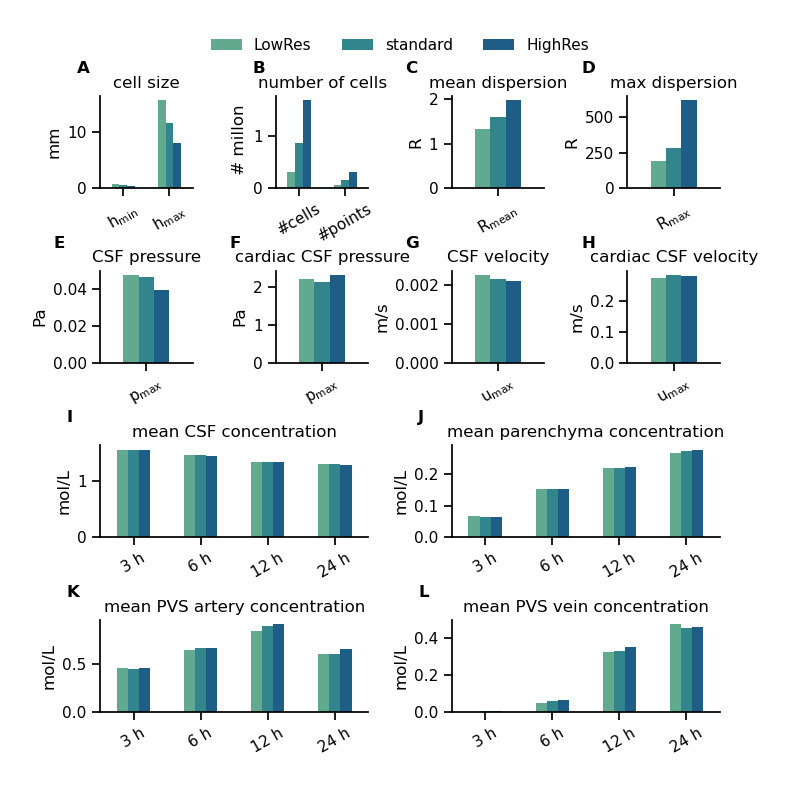
\includegraphics[width=0.9\linewidth]{figures/mesh_refinement.png}
    \caption{Illustration of the three different meshes; from left to right: low resolution, standard resolution, high resolution.}
    \label{fig:mesh_refinement}
\end{figure}

\begin{figure}
    \centering
    \begin{subfigure}[b]{0.45\textwidth}
        \centering
        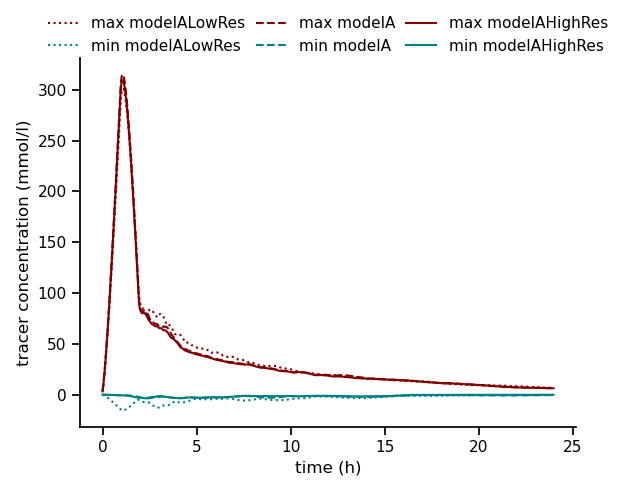
\includegraphics[width = 1 \linewidth]{figures/csf_minmax.png}
        \caption{Minimum and maximum tracer concentration in the CSF under mesh refinement}
    \end{subfigure}
    \begin{subfigure}[b]{0.45\textwidth}
        \centering
     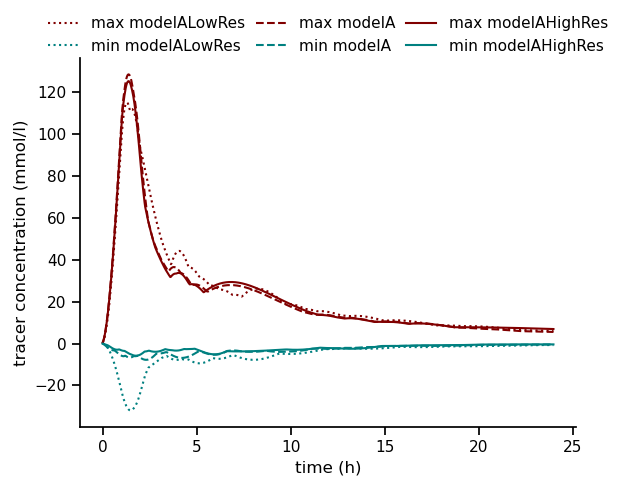
\includegraphics[width= 1 \linewidth]{figures/par_minmax.png}
        \caption{Minimum and maximum tracer concentration in the parenchyma under mesh refinement}
    \end{subfigure}
    \begin{subfigure}[b]{0.45\textwidth}
        \centering
        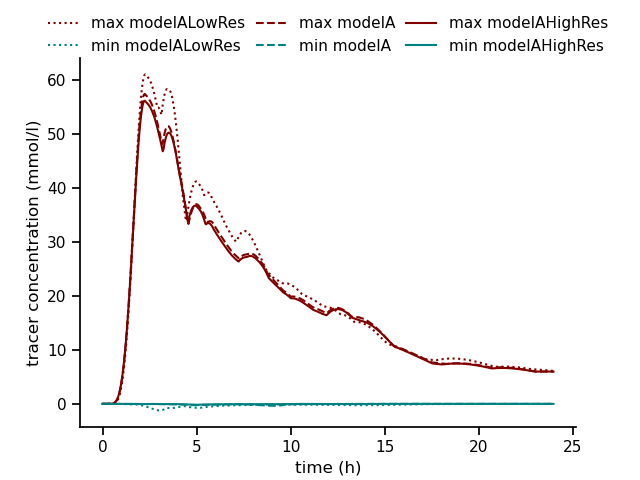
\includegraphics[width = 1 \linewidth]{figures/art_minmax.png}
        \caption{Minimum and maximum tracer concentration in PVSs around arteries under mesh refinement}
    \end{subfigure}
    \begin{subfigure}[b]{0.45\textwidth}
        \centering
     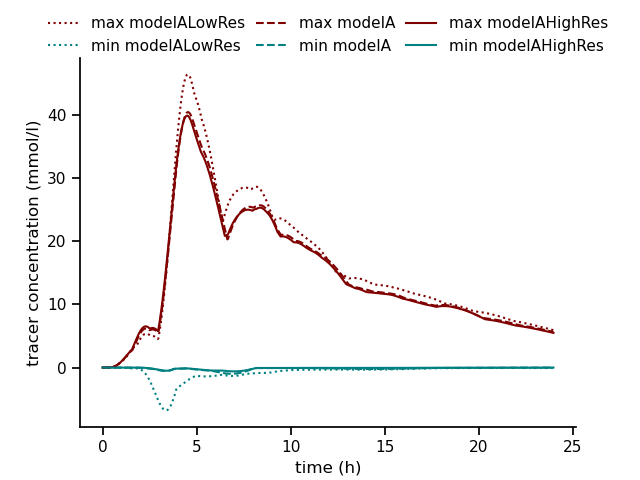
\includegraphics[width= 1 \linewidth]{figures/ven_minmax.png}
         \caption{Minimum and maximum tracer concentration in PVSs around veins under mesh refinement}
    \end{subfigure}
    \caption{Minimum and maximum tracer concentrations over the first 24\,h after injection on the CSF and parenchyma (a), and the arterial and venous PVS (b) computed on the low resolution (LowRes), standard and high resolution (HighRes) meshes with a timestep of 2 min for the baseline model (Model A).}
    \label{fig:mesh_convergence_concentrations}
\end{figure}
\begin{figure}
    \centering
    \begin{subfigure}[b]{0.49\textwidth}
        \centering
        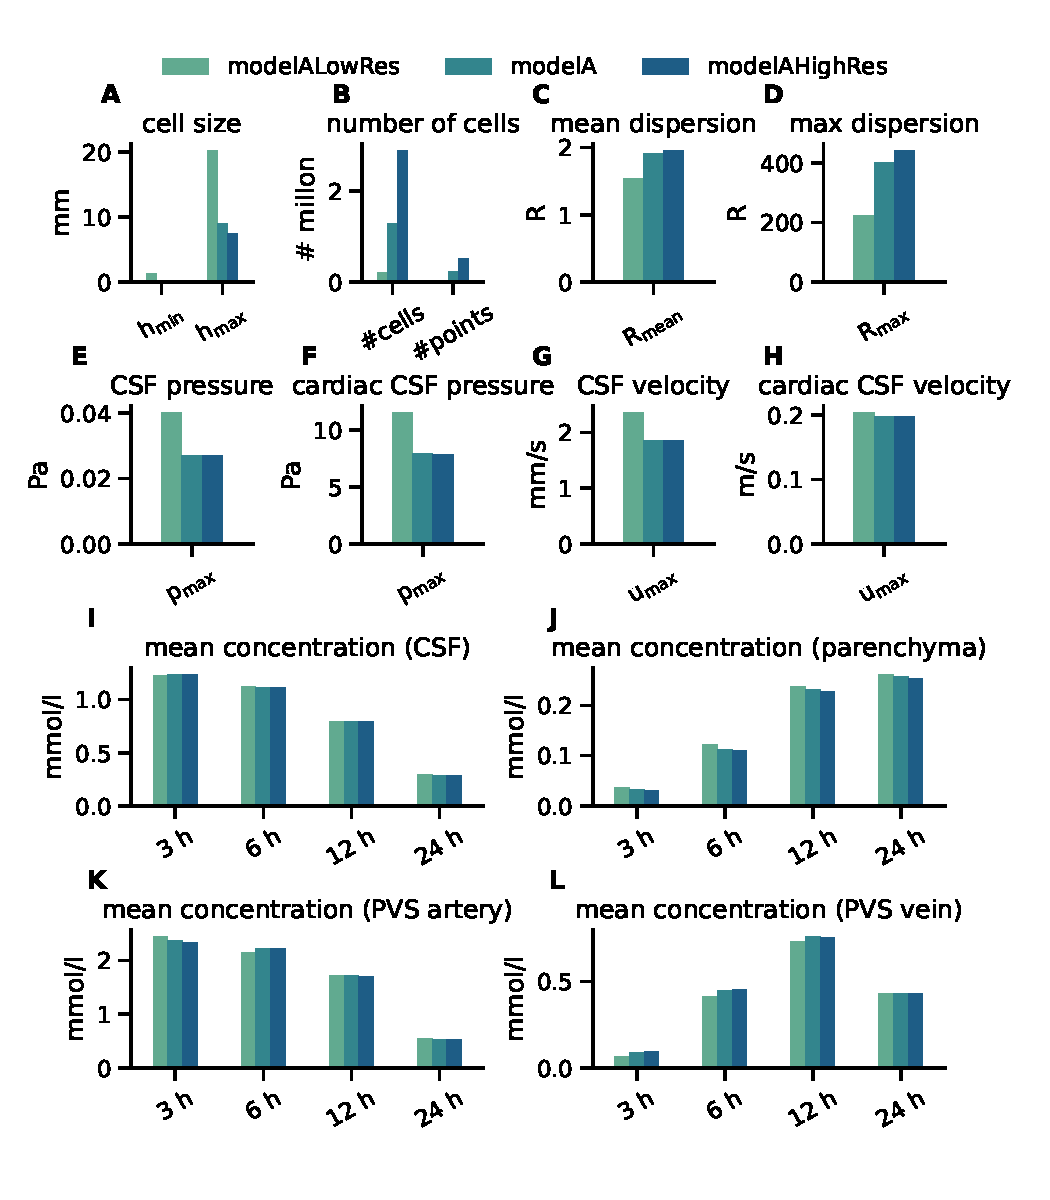
\includegraphics[trim={0.5cm 1cm 0.05cm 0.8cm}, clip, width = 1.05 \linewidth]{figures/modelALowRes_modelA_modelAHighRes.pdf}
        \caption*{Convergence of key quantities of interest with mesh refinement}
        %\label{fig:mesh_convergence}
    \end{subfigure}
    \begin{subfigure}[b]{0.49\textwidth}
        \centering
     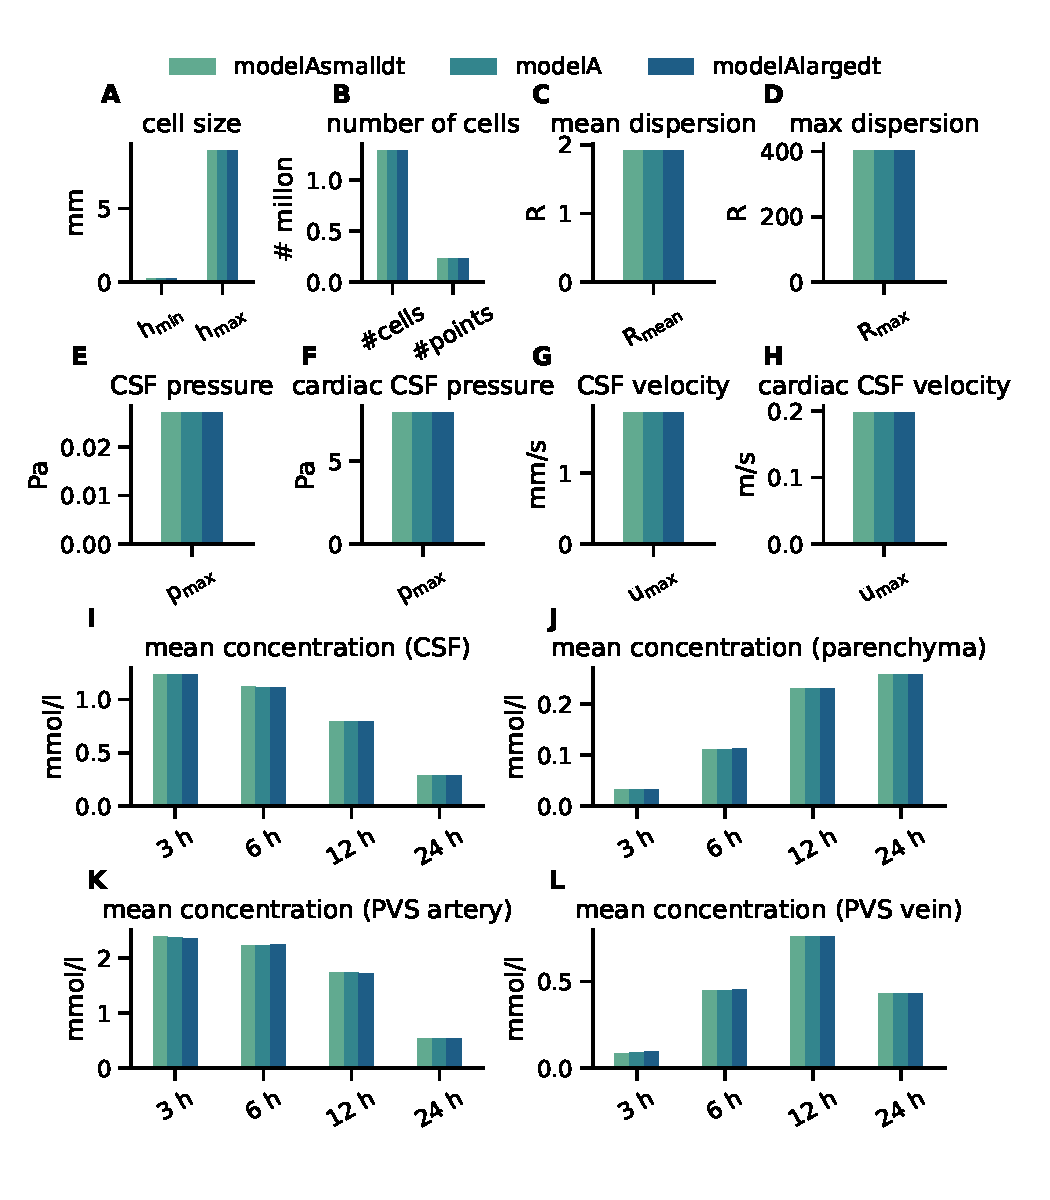
\includegraphics[trim={0.5cm 1cm 0.05cm 0.8cm}, clip,width= 1.05 \linewidth]{figures/modelAsmalldt_modelA_modelAlargedt.pdf}
        \caption*{Convergence of key quantities of interest with time refinement}
        %\label{fig:time_convergence}
    \end{subfigure}
    \caption{For both left and right panels: A: Minimal ($\rm h_{min}$) and maximal ($\rm h_{max}$) mesh cell sizes (computed as cell circumradius $\times 2$); B: number of mesh vertices and tetrahedral cells in each mesh; C: mean cardiac dispersion enhancement factor $R$; D: maximum cardiac dispersion enhancement factor $R$; E: maximum pressure in steady CSF production flow; F: maximum pressure in cardiac-driven CSF flow; G: maximum CSF velocity in steady CSF production flow; H: maximum CSF velocity in cardiac-driven CSF flow; I--L: mean tracer concentration in the CSF, parenchyma, arterial PVS and venous PVS after 3, 6, 12 and 24 hours.}
        \label{fig:mesh_time_convergence}
\end{figure}

\begin{figure}
    \centering
    \begin{subfigure}[b]{0.45\textwidth}
        \centering
        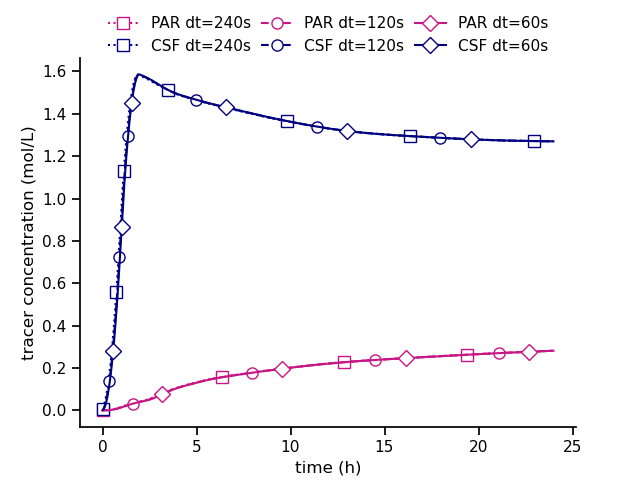
\includegraphics[width = 1 \linewidth]{figures/time_refinement_par_csf_mean.png}
        \caption{Mean tracer concentration in CSF and parenchyma under time step refinement}
    \end{subfigure}
    \begin{subfigure}[b]{0.45\textwidth}
        \centering
     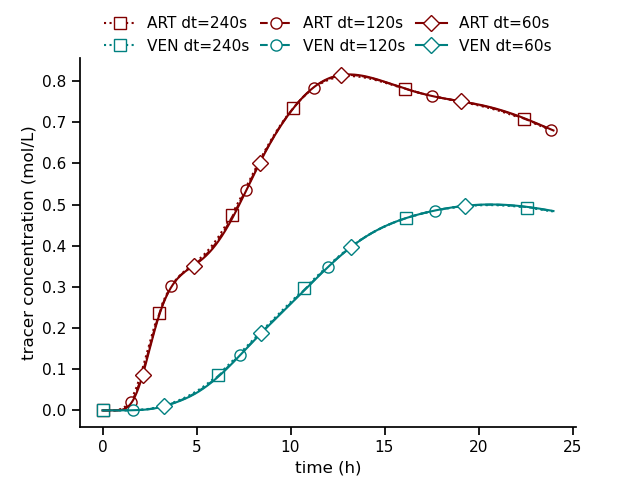
\includegraphics[width= 1\linewidth]{figures/time_refinement_art_ven_mean.png}
         \caption{Mean tracer concentration in PVSs around (veins and) arteries under time step refinement}
    \end{subfigure}
    \caption{Mean tracer concentrations after up to 24\,h in the CSF and parenchyma (a), and the arterial and venous PVS (b) computed on the standard resolution mesh for timesteps of 1, 2, and 4 minutes (dt of 60, 120, or 240 seconds)}
    \label{fig:time_convergence_concentrations}
\end{figure}
\begin{figure}
    \centering
    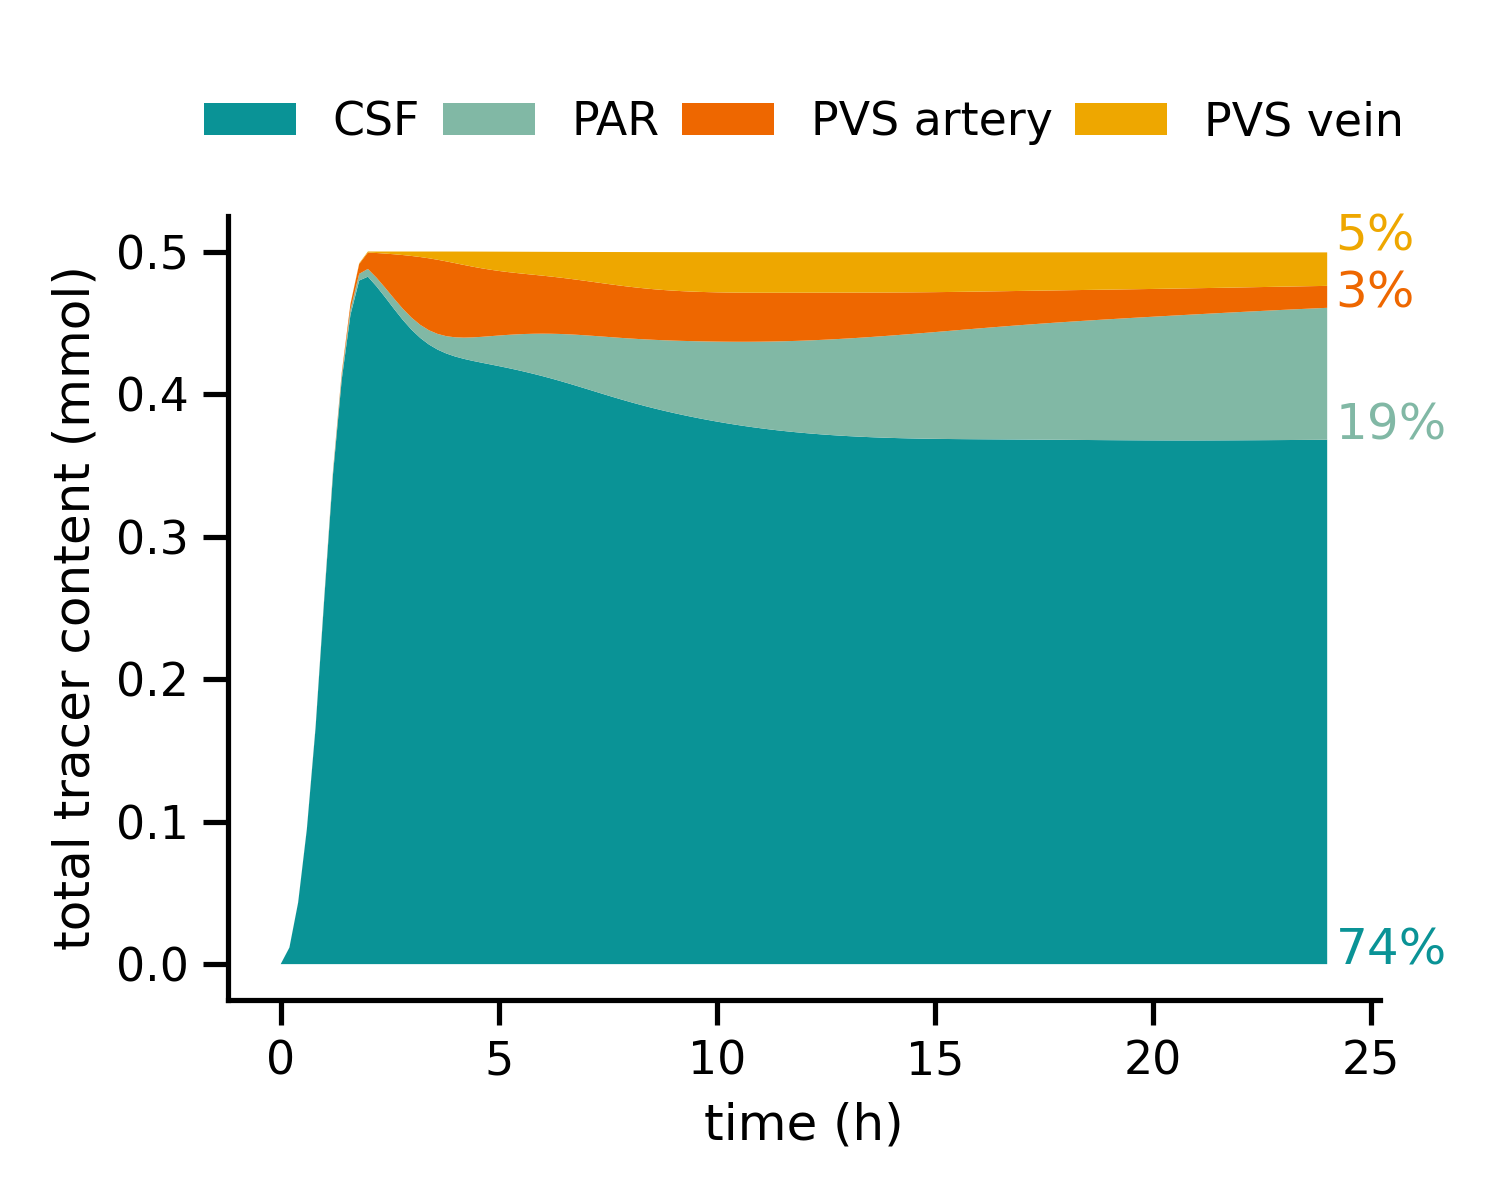
\includegraphics[width=0.5\linewidth]{figures/modelAMassConservation_total_conc.png}
    \caption{Total tracer content in the CSF, parenchyma, and arterial and venous PVS for a variant of the baseline model without tracer outflow. The total amount of tracer is constant after the initial influx phase demonstrating that the numerical scheme conserves mass globally.}
    \label{fig:mass_conservation}
\end{figure}

\section{Supplementary discussion}

\subsection{Extended model validation}
\label{sec:app:model_validation}

In addition to the comparison of our in-silico predictions of tracer
enrichment and clearance against glymphatic MRI, we here compare
auxiliary model quantities against the literature as additional model
validation.

\paragraph{CSF flow and pressures in the SAS and ventricular system}
The dynamics of human CSF flow and pressure are better quantified, by
way of clinical imaging, in-vitro studies, and computational
modelling, in other areas of the ventricular
system~\cite{linninger2007cerebrospinal, sweetman2011cerebrospinal,
  vinje2019respiratory, hornkjol2022csf, causemann2022human,
  karki2025real, liu2025transmantle}. Linninger et
al~\cite{linninger2007cerebrospinal} model CSF flow and pressure
dynamics induced by CSF production and cardiac pulsatility under
normal and hydrocephalic conditions, and report of very good agreement
with Cine (phase-contrast) MRI measurements. Our estimates of the
maximum intracranial pressure difference, 10 Pa from the cardiac
contribution and 26 mPa from CSF production, is in perfect agreement
with their maximum transmantle pressure difference of $\sim$10 Pa, and
also in very good agreement with mean pressure differences of 11.5 Pa
measured clinically between sensors placed subdurally and in the
lateral ventricle \cite{vinje2019respiratory}. Liu et
al~\cite{liu2025transmantle} report of cardiac and respiratory
pressure differences across the aqueduct of 12.1 $\pm$ 5.7 Pa and 9.5
$\pm$ 7.2 Pa, respectively; thus our baseline estimate of the respiratory contribution 1.4 Pa may be an
underestimation. On the other hand, our cardiac- and
respiratory-driven CSF flow estimates peak at 19.8 cm/s and 4.8 cm/s in the caudal direction, respectively, which are higher than phase-contrast MRI measurements of cardiac and respiratory CSF flow
components \cite{takizawa2017characterization, yildiz2017quantifying}. Some variation in CSF flow velocities is expected considering that the values from MRI represent averages
\cite{yildiz2017quantifying} and that the geometry of the CSF spaces
strongly affects peak velocities\cite{vinje2019respiratory,
  causemann2022human}. Hornkjøl et al \cite{hornkjol2022csf} model the
flow dynamics induced by CSF production in the choroid plexus and
report a peak CSF velocity of 8.9 mm/s in the aqueduct, which is 4.8
$\times$ higher than our values of 1.85 mm/s. Given that we use the
same production rate, this deviation again illustrates the impact of
potential differences in the (aqueduct) geometry on local velocities.

% Dispersion predictions
\paragraph{Dispersion in the SAS, ventricular system and PVS}
This pulsatile flow of CSF in the SAS, ventricular system and PVSs
leads to an increase in effective solute
diffusivity~\cite{stockman2007effect, hettiarachchi2011effect,
  asgari2016glymphatic, sharp2019dispersion, ray2021quantitative} via
a process known as Taylor dispersion \cite{taylor1953dispersion,
  watson1983diffusion}. Previous estimates of the magnitude of this
effect in the CSF spaces vary significantly: from an enhancement
factor of 0.05--1 in periarterial spaces surrounding penetrating
arteries~\cite{asgari2016glymphatic, troyetsky2021dispersion}, to
5--100 in the spinal subarachnoid space~\cite{stockman2007effect,
  hettiarachchi2011effect, sharp2019dispersion}, and up to more than
$10\,000$ in surface periarterial spaces~\cite{ray2021quantitative,
  sharp2019dispersion}. The large variability can (at least partly) be
attributed to methodological differences; e.g. different assumptions
on the medium, domain width, pressure differences and/or fluid
velocities, the diversity of CSF flow characteristics, as well as a
high likelihood of spatial variations. Hornkjøl et
al~\cite{hornkjol2022csf} consider model variations with constant
dispersion factors from 1 up to 1000, and indicate that a value of 10
gives the better agreement with the clinically observed
enrichment. Our spatially-varying estimates of the dispersion
enhancement factors $R_c, R_r$ (with $D = (1 + R_c + R_r) D^{\rm
  Gad}$) range from 0 to 200 for the cardiac contribution $R_c$ and 0
to 320 for the respiratory contribution $R_r$; and is thus compatible
within the previously reported spectrum.

% Effect of PVS size and shapes
\paragraph{Shapes, sizes and structures of the PVS}
The shapes, sizes and structures of the PVSs likely vary between
species (e.g.~mice vs.~humans), between spatial compartments
(e.g.~surface vs.~parenchymal), between vessel types (arteries
vs.~arterioles vs.~veins), and in
pathologies~\cite{ichimura1991distribution, foley2012realtime,
  schain2017cortical, mestre2018flow, bedussi2018paravascular,
  mestre2022periarteriolar, smets2024perivascular, raicevic2023sizes,
  vinje2021brain, eide2024functional}. In terms of shape, the PVSs are
commonly represented as annular (elliptic) cylinders, though it is
well recognized that this represents an
idealization~\cite{mestre2018flow, tithof2019hydraulic,
  vinje2021brain, raicevic2023sizes, boster2024hydraulic,
  smets2024perivascular}. In terms of sizes, Raicevic et
al~\cite{raicevic2023sizes} note that the variation in PVS area is
larger between PVS segments than along a single PVS segment and that
the PVS area increases with lumen area. In mice, reports of the ratio
between PVS and lumen area range from
$\approx$0.35--0.43~\cite{smets2024perivascular} up to
$\approx$1.12--1.4~\cite{raicevic2023sizes, mestre2018flow}. In
humans, the PVS may be as wide as the associated surface artery and up
to 4$\times$ wider in iNPH subjects~\cite{eide2024functional}, which
would correspond to substantially larger PVS area ratios (3 or
higher). To reflect the human scale, we here represent each PVS
segment as an annular cylinder with inner radius $R_1$ and outer
radius $R_2$ of width and area proportional to that of the
corresponding blood vessel ($R_2 = 2 R_1$ at baseline, $R_2 = 3 R_1$
for enlarged PVS). The hydraulic resistance of annular cross-sections
is $1-6 \times$~\cite{tithof2019hydraulic} larger than more elongated
cross-sections and thus our estimates of the pressure-induced PVS
velocities are conservative.

%\paragraph{Predictions on overall tracer spreading patterns}

%We compare our in-silico predictions with clinical data from human subjects, in particular the studies by Ringstad et al~\cite{ringstad2018brain}, Watts et al~\cite{watts2019measuring} and Eide and Ringstad~\cite{eide2024functional}. Finding an overall good agreement, we provide a detailed overview on key quantities of interest in %FTA in MCA2 & N/A & N/A & 53.1 ± 50.5 min & 2:12 / 1:48 hours +$t_{st}$ \\
%FTA in ACA2 & N/A & N/A & 48.3 ± 46.1 min & 3:00 hours +$t_{st}$ \\
%\bottomrule
%\end{tabular}
%\caption{Comparison of clinical studies and model predictions on tracer spreading patterns %and arrival times.}
%\label{tab:spreading_comparison}
%\end{table}


\end{document}
